% Arquivo LaTeX de exemplo de dissertação/tese a ser apresentados à CPG do IME-USP
%
% Versão 5: Sex Mar  9 18:05:40 BRT 2012
%
% Criação: Jesús P. Mena-Chalco
% Revisão: Fabio Kon e Paulo Feofiloff
%
% Obs: Leia previamente o texto do arquivo README.txt

\documentclass[12pt,twoside,a4paper]{book}

% ---------------------------------------------------------------------------- %
% Pacotes
\usepackage[utf8]{inputenc}
\usepackage[T1]{fontenc}
\usepackage[english]{babel}
\usepackage[pdftex]{graphicx}           % usamos arquivos pdf/png como figuras
\usepackage{setspace}                   % espaçamento flexível
\usepackage{indentfirst}                % indentação do primeiro parágrafo
\usepackage{makeidx}                    % índice remissivo
\usepackage[nottoc]{tocbibind}          % acrescentamos a bibliografia/indice/conteudo no Table of Contents
\usepackage{sourcecodepro}
\usepackage{type1cm}                    % fontes realmente escaláveis
\usepackage{listings}                   % para formatar código-fonte (ex. em Java)
\usepackage{titletoc}
\usepackage{booktabs}
\usepackage{textcomp}
\usepackage[explicit]{titlesec} % cabeçalhos dos títulos: menores e compactos
\usepackage[bold,full]{complexity}
\usepackage{tocloft}
\usepackage{amssymb}
\usepackage{amsmath}
\usepackage{relsize}
\usepackage{epigraph}
\usepackage[fixlanguage]{babelbib}
\usepackage[font=small,format=plain,labelfont=bf,up,textfont=it,up]{caption}
\usepackage[usenames,svgnames,dvipsnames,table,xcdraw]{xcolor}
\usepackage{wrapfig}
\usepackage[a4paper,top=2.54cm,bottom=2.0cm,left=2.0cm,right=2.54cm]{geometry} % margens
%\usepackage[pdftex,plainpages=false,pdfpagelabels,pagebackref,colorlinks=true,citecolor=black,linkcolor=black,urlcolor=black,filecolor=black,bookmarksopen=true]{hyperref} % links em preto
\usepackage[pdftex,plainpages=false,pdfpagelabels,pagebackref,colorlinks=true,citecolor=DarkGreen,linkcolor=NavyBlue,urlcolor=DarkRed,filecolor=green,bookmarksopen=true]{hyperref} % links coloridos
\usepackage[all]{hypcap}                    % soluciona o problema com o hyperref e capitulos
\usepackage[round,sort,nonamebreak,numbers]{natbib} % citação bibliográfica textual(plainnat-ime.bst)
\usepackage{todonotes}
%\fontsize{60}{62}\usefont{OT1}{cmr}{m}{n}{\selectfont}
\setlength{\epigraphrule}{0pt}
\setlength{\epigraphwidth}{8cm}
\renewcommand{\textflush}{flushepinormal}

% ---------------------------------------------------------------------------- %
% Cabeçalhos similares ao TAOCP de Donald E. Knuth
\usepackage{fancyhdr}
\pagestyle{fancy}
\fancyhf{}
\renewcommand{\chaptermark}[1]{\markboth{#1}{}}
\renewcommand{\sectionmark}[1]{\markright{#1}}
\renewcommand{\headrulewidth}{0pt}

\fancyhead[LE,RO]{\thepage}
\fancyhead[LO]{\itshape\nouppercase{\rightmark}}
\fancyhead[RE]{\itshape\nouppercase{\leftmark}}

% ---------------------------------------------------------------------------- %
\graphicspath{{./images/}}             % caminho das figuras (recomendável)
\frenchspacing                          % arruma o espaço: id est (i.e.) e exempli gratia (e.g.)
\urlstyle{same}                         % URL com o mesmo estilo do texto e não mono-spaced
\makeindex                              % para o índice remissivo
\raggedbottom                           % para não permitir espaços extra no texto
%\fontsize{60}{62}\usefont{OT1}{cmr}{m}{n}{\selectfont}
\cleardoublepage
\normalsize

% ---------------------------------------------------------------------------- %
% Opções de listing usados para o código fonte
% Ref: http://en.wikibooks.org/wiki/LaTeX/Packages/Listings
\lstset{ %
language=Java,                  % choose the language of the code
basicstyle=\footnotesize,       % the size of the fonts that are used for the code
numbers=left,                   % where to put the line-numbers
numberstyle=\footnotesize,      % the size of the fonts that are used for the line-numbers
stepnumber=1,                   % the step between two line-numbers. If it's 1 each line will be numbered
numbersep=5pt,                  % how far the line-numbers are from the code
showspaces=false,               % show spaces adding particular underscores
showstringspaces=false,         % underline spaces within strings
showtabs=false,                 % show tabs within strings adding particular underscores
frame=single,                    % adds a frame around the code
framerule=0.6pt,
tabsize=2,                        % sets default tabsize to 2 spaces
captionpos=b,                   % sets the caption-position to bottom
breaklines=true,                % sets automatic line breaking
breakatwhitespace=false,        % sets if automatic breaks should only happen at whitespace
escapeinside={\%*}{*)},         % if you want to add a comment within your code
backgroundcolor=\color[rgb]{1.0,1.0,1.0}, % choose the background color.
rulecolor=\color[rgb]{0.8,0.8,0.8},
extendedchars=true,
xleftmargin=10pt,
xrightmargin=10pt,
framexleftmargin=10pt,
framexrightmargin=10pt
}

% Setting Chapter Style
\makeatletter
\def\thickhrulefill{\leavevmode \leaders \hrule height .1ex \hfill \kern \z@}
\def\@makechapterhead#1{%
  %\vspace*{50\p@}%
  %\vspace*{5\p@}%
  {\parindent \z@ \centering \reset@font
        \thickhrulefill\quad
        \itshape \bfseries \normalsize \@chapapp{} \thechapter
        \normalsize \quad \thickhrulefill
        \par\nobreak
        \vspace*{5\p@}%
        \interlinepenalty\@M
        %\hrule
        %\vspace*{10\p@}%
        \normalfont \LARGE \bfseries #1\par\nobreak
        \par
        \vspace*{5\p@}%
        %\hrule
    %\vskip 40\p@
    \vskip 30\p@
  }}
\def\@makeschapterhead#1{%
  %\vspace*{50\p@}%
  %\vspace*{5\p@}%
  {\parindent \z@ \centering \reset@font
        \thickhrulefill
        \par\nobreak
        \vspace*{5\p@}%
        \interlinepenalty\@M
        %\hrule
        %\vspace*{10\p@}%
        \LARGE \bfseries #1\par\nobreak
        \par
        \vspace*{5\p@}%
        %\hrule
    %\vskip 40\p@
    \vskip 30\p@
  }}

\renewcommand\cftloftitlefont{\itshape\bfseries\Large}

\renewcommand\cftlottitlefont{\itshape\bfseries\Large}

\renewcommand\cfttoctitlefont{\hfill\itshape\bfseries\Large}

\renewcommand{\cftaftertoctitle}{\hfill}

 \titleformat{\section}
  {\itshape\large\bfseries}{\thesection}{1em}{#1}

\titleformat{\subsection}
  {\itshape\normalsize\bfseries}{\thesubsection}{1em}{#1}

\titleformat{\subsubsection}
  {\normalsize\bfseries\itshape}{\thesubsubsection}{1em}{#1}

% Setting custom lists
%\newcommand{\listabbreviationname}{\itshape \Large List of Abbreviations}
%
%\newlistof{abbreviation}{abb}{\listabbreviationname}
%
%\newcommand{\abbreviation}[2]{%
%\refstepcounter{abbreviation}
%%\par\noindent\textbf{Example \theexample. #1}
%\addcontentsline{abb}{abbreviation}
%{\protect\makebox[2cm]{#1} #2}\par}
%
%\cftpagenumbersoff{abbreviation}
%
%% Setting custom lists
%\newcommand{\listsymbolentryname}{\itshape \Large List of Symbols}
%
%\newlistof{symbolentry}{synt}{\listsymbolentryname}
%
%\newcommand{\symbolentry}[2]{%
%\refstepcounter{symbolentry}
%%\par\noindent\textbf{Example \theexample. #1}
%\addcontentsline{synt}{symbolentry}
%{\protect\makebox[2cm]{#1} #2}\par}
%
%\cftpagenumbersoff{symbolentry}
%
\setcitestyle{square}

% ---------------------------------------------------------------------------- %
% Corpo do texto
\begin{document}
\frontmatter
% cabeçalho para as páginas das seções anteriores ao capítulo 1 (frontmatter)
%\fancyhead[RO]{{\footnotesize\rightmark}\hspace{2em}\thepage}
\setcounter{tocdepth}{2}
%\fancyhead[LE]{\thepage\hspace{2em}\footnotesize{\leftmark}}
%\fancyhead[RE,LO]{}
%\fancyhead[RO]{{\footnotesize\rightmark}\hspace{2em}\thepage}

\onehalfspacing  % espaçamento

% ---------------------------------------------------------------------------- %
% CAPA
% Nota: O título para as dissertações/teses do IME-USP devem caber em um
% orifício de 10,7cm de largura x 6,0cm de altura que há na capa fornecida pela SPG.
\thispagestyle{empty}
\begin{center}
    \vspace*{2.3cm}
    \textbf{\Large{Parallel and Distributed Autotuning \\
                   for High-Performance Computing}}\\

    \vspace*{1.2cm}
    \Large{Pedro Bruel}

    \vskip 2cm
    \textsc{
    Text submitted\\[-0.25cm]
    to the\\[-0.25cm]
    Institute de Mathematics and Statistics\\[-0.25cm]
    of the\\[-0.25cm]
    University of São Paulo\\[-0.25cm]
    for the\\[-0.25cm]
    Qualifying examination\\[-0.25cm]
    for the\\[-0.25cm]
    Doctoral Degree in\\[-0.25cm]
    Computer Science}

    \vskip 1.5cm
    Advisor: Professor Alfredo Goldman Vel Lejbman

       \vskip 1cm
    \normalsize{During the development of this work, the author was supported
    by CNPq \textnumero XXXX, Hewlett-Packard Enterprise and CAPES}

    \vskip 0.5cm
    \normalsize{São Paulo, \today}
\end{center}

% ---------------------------------------------------------------------------- %
% Página de rosto (SÓ PARA A VERSÃO DEPOSITADA - ANTES DA DEFESA)
% Resolução CoPGr 5890 (20/12/2010)
%
% IMPORTANTE:
%   Coloque um '%' em todas as linhas
%   desta página antes de compilar a versão
%   final, corrigida, do trabalho
%
%
\newpage
\thispagestyle{empty}
    \begin{center}
        \vspace*{2.3 cm}
        \textbf{\Large{Parallel and Distributed Autotuning\\
                       for High-Performance Computing}}\\
        \vspace*{2 cm}
    \end{center}

    \vskip 2cm

    \begin{flushright}
    This is the original version\\
    submitted for evaluation\\
    by Pedro Bruel
    \end{flushright}

\pagebreak


% ---------------------------------------------------------------------------- %
% Página de rosto (SÓ PARA A VERSÃO CORRIGIDA - APÓS DEFESA)
% Resolução CoPGr 5890 (20/12/2010)
%
% Nota: O título para as dissertações/teses do IME-USP devem caber em um
% orifício de 10,7cm de largura x 6,0cm de altura que há na capa fornecida pela SPG.
%
% IMPORTANTE:
%   Coloque um '%' em todas as linhas desta
%   página antes de compilar a versão do trabalho que será entregue
%   à Comissão Julgadora antes da defesa
%
%
%\newpage
%\thispagestyle{empty}
%    \begin{center}
%        \vspace*{2.3 cm}
%        \textbf{\Large{Título do trabalho a ser apresentado à \\
%        CPG para a dissertação/tese}}\\
%        \vspace*{2 cm}
%    \end{center}
%
%    \vskip 2cm
%
%    \begin{flushright}
%    Esta versão da dissertação/tese contém as correções e alterações sugeridas\\
%    pela Comissão Julgadora durante a defesa da versão original do trabalho,\\
%    realizada em xx/xx/2017. Uma cópia da versão original está disponível no\\
%    Instituto de Matemática e Estatística da Universidade de São Paulo.
%
%    \vskip 2cm
%
%    \end{flushright}
%    \vskip 4.2cm
%
%    \begin{quote}
%    \noindent Comissão Julgadora:
%
%    \begin{itemize}
%        \item Profª. Drª. Nome Completo (orientadora) - IME-USP [sem ponto final]
%        \item Prof. Dr. Nome Completo - IME-USP [sem ponto final]
%        \item Prof. Dr. Nome Completo - IMPA [sem ponto final]
%    \end{itemize}
%
%    \end{quote}
%\pagebreak


\pagenumbering{roman}     % começamos a numerar

% ---------------------------------------------------------------------------- %
% Agradecimentos:
% Se o candidato não quer fazer agradecimentos, deve simplesmente eliminar esta página
%\chapter*{Agradecimentos}
%Texto texto texto texto texto texto texto texto texto texto texto texto texto
%texto texto texto texto texto texto texto texto texto texto texto texto texto
%texto texto texto texto texto texto texto texto texto texto texto texto texto
%texto texto texto texto. Texto opcional.


% ---------------------------------------------------------------------------- %
% Resumo
%\chapter*{Resumo}
%
%\noindent BRUEL, P. \textbf{Título do trabalho em português}.
%2017. xxx f.
%Qualificação (Doutorado) - Instituto de Matemática e Estatística,
%Universidade de São Paulo, São Paulo, 2010.
%\\
%
%Elemento obrigatório, constituído de uma sequência de frases concisas e
%objetivas, em forma de texto.  Deve apresentar os objetivos, métodos empregados,
%resultados e conclusões.  O resumo deve ser redigido em parágrafo único, conter
%no máximo 500 palavras e ser seguido dos termos representativos do conteúdo do
%trabalho (palavras-chave).
%\\
%
%\noindent \textbf{Palavras-chave:} palavra-chave1, palavra-chave2, palavra-chave3.
%
%\vspace*{1cm}%
%\thickhrulefill

% ---------------------------------------------------------------------------- %
% Abstract
\chapter*{Abstract}
\noindent BRUEL, P. \textbf{Parallel and Distributed Autotuning for High-Performance Computing}.
2017. xxx f.
Qualifying Examination (PhD) - Institute of Mathematics and Statistics,
University of São Paulo, São Paulo, 2017.
\\


Elemento obrigatório, elaborado com as mesmas características do resumo em
língua portuguesa. De acordo com o Regimento da Pós- Graduação da USP (Artigo
99), deve ser redigido em inglês para fins de divulgação.
\\

\noindent \textbf{Keywords:} keyword1, keyword2, keyword3.

\vspace*{1cm}%
\thickhrulefill

\newpage
% ---------------------------------------------------------------------------- %
% Sumário
\tableofcontents    % imprime o sumário

% ---------------------------------------------------------------------------- %
%\newpage
%\symbolentry{$\omega$}{Frequência angular}
%\symbolentry{$\psi$}{Função de análise \emph{wavelet}}
%\symbolentry{$\Psi$}{Transformada de Fourier de $\psi$}
%\begin{NoHyper}
%\listofsymbolentry
%\end{NoHyper}
%\addcontentsline{toc}{chapter}{List of Symbols}
%\newpage
%
%% ---------------------------------------------------------------------------- %
%
%% Listas de figuras e tabelas criadas automaticamente
%\newpage
%\abbreviation{CFT}{Transformada contínua de Fourier (\emph{Continuous Fourier Transform})}
%\abbreviation{DFT}{Transformada discreta de Fourier (\emph{Discrete Fourier Transform})}
%\abbreviation{EIIP}{Potencial de interação elétron-íon (\emph{Electron-Ion Interaction Potentials})}
%\abbreviation{STFT}{Tranformada de Fourier de tempo reduzido (\emph{Short-Time Fourier Transform})}
%\begin{NoHyper}
%\listofabbreviation
%\end{NoHyper}
%\addcontentsline{toc}{chapter}{List of Abbreviations}
%\newpage

\listoffigures

\listoftables

% ---------------------------------------------------------------------------- %
% Capítulos do trabalho
\mainmatter

% cabeçalho para as páginas de todos os capítulos
%\fancyhead[RE,LO]{\thesection}

%\singlespacing              % espaçamento simples
\onehalfspacing            % espaçamento um e meio

\chapter{Introduction}
\label{chap:introduction}

The search for more computational power leads to a series of challenges.
Quantum tunneling effects and the speed of light influence the size of
transistors and the length of circuits, and compel the development of
multi-core and heterogeneous computer architectures.  Battery life and a
responsible use of natural resources influence circuit frequency and power
consumption, and compel the development of dynamic frequency scaling and
cooling solutions.  Comparably, the selection and configuration of the
algorithms and computer architectures influence the performance they achieve,
and compel the development of automated selection and configuration solutions.

The use of heterogeneous programming models and computer architectures in High
Performance Computing has increased despite the difficulty of optimizing and
configuring legacy code, and of developing new solutions for heterogeneous
computing. Due to the great diversity of programming models and architectures,
there is no single optimization strategy that fits all problems and
architectures.

An optimization solution tailored for a specific problem requires time and
expert knowledge. Using general optimizations is faster and cheaper, often at
the cost of application-specific performance improvements. A possible solution
to this trade-off is the automation of the program optimization process.

The automated selection of algorithms and configuration of programs, referred
to as \textit{autotuning} from now on, casts the program optimization problem
as a search problem. The possible configurations and optimizations of a program
are used to compose a \textit{search space}, and searching is done by
evaluating the impact of each configuration on the initial program.  Using the
increasingly available computing power to measure different versions of a
program, an \textit{autotuner} searches for good selections, configurations,
and optimizations. The measurements must quantify a meaningful metric for the
programmer, such as execution time and memory or power consumption.

From the implementation in a high-level programming language to the instruction
selection in code generation, it is possible to expose optimization and
configuration opportunities in various stages of program development and
execution.  The time to measure the results of an optimization choice depends
on the selected stage and on the metric to be optimized.

\todo[inline,author=Pedro,color=cyan]{Describe variety of heterogeneous
architectures: NUMA, memory centric, ...}

\todo[inline,author=Pedro,color=cyan]{Show some example: (Genetic Algorithm,
Sorting, Compiler Flag, LLVM Pass)?}

Different steps of a program's development and deployment can be optimized.
Some steps can be more expensive to measure and therefore optimize.  For
example, access to certain architectures might be costly and limited, or it may
take a long time to solve certain problem instances.
\todo[inline,author=Pedro,color=cyan]{Examples: GPU \& CPU compilation,
FPGA hardware generation, compilation for supercomputers, ...}

\todo[inline,author=Pedro,color=cyan]{How to autotune:
 Complex systems, such as HACC?;
 Programs for a supercomputer, like the Titan?;
 FPGA compilation?;
 Hardware and software co-design?}

\todo[inline,author=Pedro,color=cyan]{Current autotuning approaches:
 Require multiple expensive evaluations;
 Do not leverage parallel and distributed computing;
 Not flexible to target multiple development and execution steps}

\section{Objectives and Expected Contributions}
\label{sec:contributions}

\todo[inline,author=Pedro,color=cyan]{A new approach must:
 Leverage distributed and parallel computing power;
 Target different steps of development and execution;
 Handle expensive to measure cases efficiently}

\todo[inline,author=Pedro,color=cyan]{Our expected contribution
is advancing the state-of-the-art of autotuning tools,
leveraging distributed and parallel computing to perform
autotuning in a variety of HPC domains}

\todo[inline,author=Pedro,color=cyan]{Briefly describe the
Julia system}

\section{Efforts for a Reproducible and Open Research}

We believe openness and reproducibility are fundamental to the quality of
Computer Science research. We made efforts to ensure our research is
reproducible and open, and we believe these efforts help our conclusions.  In
this section we describe the efforts we made.

To ensure the openness of our research we uploaded the software developed
during and for research to public hosting services. We used version control
tools and made the code available under free software licenses. We also
made available the copyright-free versions of our papers, which is a common
practice in Computer Science. The research we performed is free to be used and
modified by future researchers.

To ensure the reproducibility of our research we included hardware and software
specifications in our reports and papers. We uploaded the code to generate the
data, text, presentations and data visualizations to public hosting services.
This code is also available under free-software licenses. Researchers are able
to reproduce our results if they have access to the architecture and software
we specify.

Unfortunately, not all of our research could be made open. The hardware
implementations for the CPUs, GPUs, FPGAs and most electronic components used
to produce our results are not made available by their manufacturers. Neither
is the software used to generate FPGA hardware from its Verilog specification.
To ensure reproducibility in these cases we disclosed the hardware
vendor-specified names and characteristics, and the versions of closed software
we used.

With these efforts for a reproducible and open research we believe we have
provided a better foundation for our conclusions and expected contributions.

\section{Text Structure}
\label{sec:org}

\todo[inline,author=Pedro,color=cyan]{Describe each chapter (and
the papers attached to end of the document?)}

\chapter{Autonomous Search \& Autotuning}
\label{chap:autonomous}
\epigraph{\textit{There is nothing like looking, if you want to find something. You
certainly usually find something, if you look, but it is not always quite the
something you were after.}}{--- J.R.R. Tolkien, \textit{The Hobbit}}


\section{Algorithm Selection and Autonomous Solvers}
\label{sec:algselres}

In 1976 John R. Rice published \textit{The Algorithm
Problem}~\cite{rice1976algorithm}, an influential paper where he formulated
abstract models for the problem of selecting effective algorithms for a given
problem. In Rice's framework the objective is to select the best algorithm,
according a performance metric, for a given problem. Consider a \textit{problem
space} $P$, and a problem $x \in P$.

Figure~\ref{fig:riceframe} presents Rice's algorithm selection
framework.

\begin{figure}[htpb]
    \begin{center}
        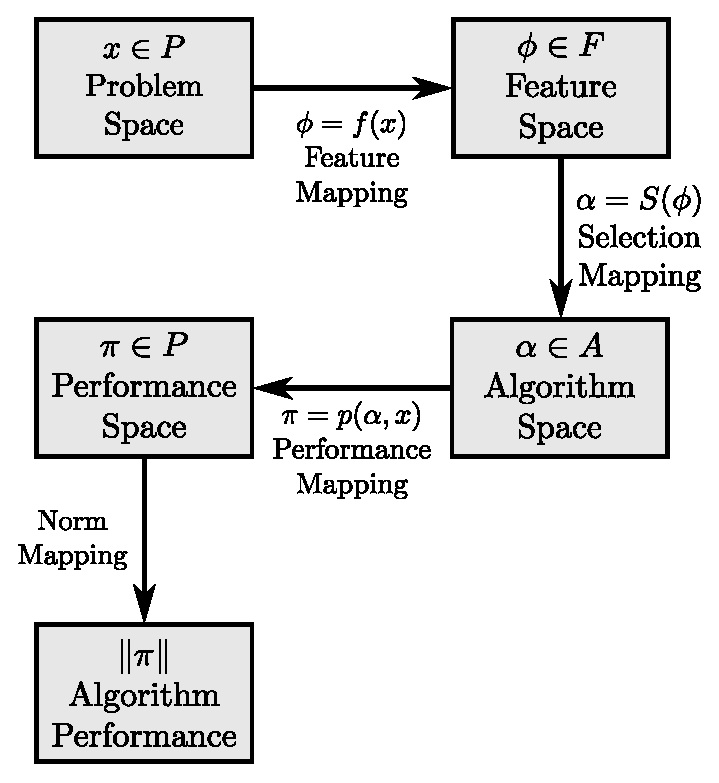
\includegraphics[width=.35\textwidth]{algorithm-selection}
    \end{center}
    \caption{Rice's framework}
    \label{fig:riceframe}
\end{figure}

\todo[inline,author=Pedro,color=cyan]{Discuss autonomous solvers}
\todo[inline,author=Pedro,color=cyan]{Discuss the choice of autotuning for
this work, given all the possibilities for solving the same problem
presented in this chapter}

\section{On-line Control}
\label{sec:oncontrol}

\subsection{Adaptive Parameter Configuration}
\label{subsec:paramadaptive}

\subsection{Credit Assignment}
\label{subsec:creditassign}

\subsection{Reinforcement Learning}
\label{subsec:reinforce}

\section{Off-line Configuration}
\label{sec:offconfig}

\subsection{Evolutionary Computing}
\label{subsec:evolcomp}

\subsection{Stochastic Local Search}
\label{subsec:searchsls}

\subsection{Machine Learning}
\label{subsec:searchml}

\section{Autotuning}
\label{chap:autotuning}

Rice's conceptual framework~\cite{rice1976algorithm} formed the foundation
of autotuners in various problem domains.  In 1997, the PHiPAC
system~\cite{bilmes1997optimizing} used code generators and search scripts to
automatically generate high performance code
for matrix multiplication. Since then, systems tackled different domains with a
diversity of strategies. Whaley \emph{et al.}~\cite{dongarra1998automatically}
introduced the ATLAS project, that optimizes dense matrix multiplication
routines. The OSKI~\cite{vuduc2005oski} library provides automatically tuned
kernels for sparse matrices. The FFTW~\cite{frigo1998fftw} library provides
tuned C subroutines for computing the Discrete Fourier Transform.
Periscope~\cite{gerndt2010automatic} is a distributed online autotuner for
parallel systems and single-node performance.

\begin{table}[htpb]
    \centering
    \begin{tabular}{@{}lll@{}}
        \toprule
        System & Domain & Technique \\ \midrule
        OSKI~\cite{vuduc2005oski} & Sparse Linear Algebra & Heuristic + Exhaustive \\
        LGen~\cite{spampinato2014basic} & Small-scale Linear Algebra & Exhaustive + Random \\
        ATLAS~\cite{dongarra1998automatically} & Dense Linear Algebra & Exhaustive \\
        INSIEME~\cite{jordan2012multi} & Compiler & Genetic Algorithm \\
        Petabricks~\cite{ansel2009petabricks} & Domain-Agnostic & Genetic Algorithm\\
        TANGRAM~\cite{chang2016efficient} & Heterogeneous Architectures & Breadth-First Search + Pruning \\
        SPIRAL~\cite{puschel2005spiral} & DSP Algorithms & Pareto Active Learning \\
        GCC Milepost~\cite{fursin2011milepost} & Compiler & Central DB + Machine Learning \\
        Apollo~\cite{beckingsale2017apollo} & GPU kernels & Decision Trees \\
        Active Harmony~\cite{tapus2002active} & Runtime & Nelder-Mead \\
        MASE-BDI~\cite{coelho2016mase} & Environmental Land Change & Distributed Active Harmony~\cite{tapus2002active} \\
        ParamILS~\cite{hutter2009paramils} & Domain-Agnostic & Stochastic Local Search \\
        CLTune~\cite{nugteren2015cltune} & OpenCL kernels & Stochastic Local Search\\
        OpenTuner~\cite{ansel2014opentuner} & Domain-Agnostic & Ensemble \\
        Periscope~\cite{gerndt2017multi} & HPC Applications & Various \\
        \bottomrule
    \end{tabular}
    \caption{Selected autotuning systems, their domains and techniques}
\end{table}

\subsection{Exhaustive Search \& Heuristics}

Abdelfattah et al.~\cite{abdelfattah2016performance} present an autotuning
strategy using exhaustive evaluation of General Matrix-Matrix Multiply (GEMM)
kernel optimizations for GPUs. They later use this approach to optimize GPU
kernels for large-scale tensor contractions~\cite{abdelfattah2016high}.
Guerreiro et al.~\cite{guerreiro2015multi} use search space pruning strategies
and exhaustive evaluation to autotune CUDA GPU kernels.  Garvey et
al.~\cite{garvey2015automatic} present a strategy to autotune OpenCL GPU
kernels using machine learning, heuristics for search space partitioning and
exhaustive search.  PolyMage~\cite{mullapudi2015polymage} is a domain-specific
language and compiler for image processing pipelines. It uses heuristics and
performance models to prune the search space, which is then explored
exhaustively.  LGen~\cite{spampinato2014basic} is a compiler for small-scale
linear algebra computation that uses mathematical domain-specific languages to
optimize loops and vectorization. LGen uses exhaustive or random search to test
different optimizations.

\subsection{Genetic Algorithms}

Ziegler et al.~\cite{ziegler2016synthesis,ziegler2016scalable} present an
autotuning system for hardware synthesis parameters that uses genetic and
learning algorithms to explore the hardware design space for real industrial
chip designs from IBM.  In an effort to provide a common representation of
multiple parallel programming models, the INSIEME compiler
project~\cite{jordan2012multi} implements abstractions for OpenMP, MPI and
OpenCL, and generates optimized parallel code for heterogeneous multi-core
architectures.

\subsection{Machine Learning}

Tartara and Reghizzi~\cite{tartara2012parallel} use the MapReduce programming
model to improve the performance of machine learning algorithms in the
PetaBricks compiler. Later they presented a machine learning
algorithm~\cite{tartara2013continuous} that learns compiler heuristics using
data gathered after every compilation.  Ngoko et al.~\cite{ngoko2016automatic}
introduce an autotuning system for $\NP$-hard problems that uses distributed
measurements of configurations and machine learning algorithms aided by
randomization, clustering and set intersection solvers.  Luo et
al.~\cite{luo2015fast} present a framework for stencil computations that uses
Optimal-Solution Spaces, input feature extraction and machine learning.
Mametjanov et al.~\cite{mametjanov2015autotuning} present an autotuning
approach that uses machine learning and selective sampling of the search space
to optimize FPGA hardware design parameters for performance and power.  Hou et
al.~\cite{hou2017auto} present an autotuning framework that uses decision trees
to optimize the sparse matrix-vector multiply kernel for multi and many-core
processors.  Apollo~\cite{beckingsale2017apollo} is an autotuning framework for
input-dependent kernels that uses a decision tree classifier that provides
optimizations that can be selected during runtime.

\subsection{Model-aided}

TuningGenie~\cite{ivanenko2014method} presents an autotuning framework that
uses code annotations and an analytical model for generating autotuners for
parallel programs.  Falsch and Elster~\cite{falch2017machine} build performance
models for OpenCL applications in different target architectures using machine
learning.  A statistical model learned and later used to pick promising
configurations for testing.  Balaprakash et al.~\cite{balaprakash2016automomml}
introduce a framework that uses machine learning algorithms to build models for
metrics such as performance and energy consumption, which are used for
multi-objective optimization.
Lang~\cite{lang2017data} reviews work on autotuning based on analytical
performance models, arguing that the approach is feasible.
Xu et al.~\cite{xu2016analytical} introduce an autotuning framework for
loop scheduling in GPUs that uses analytical performance models.

Shuchart et al.~\cite{schuchart2017readex} introduce the READEX (Runtime
Exploitation of Application Dynamism for Energy-efficient eXascale computing)
project and its methodology for developing tools to improve the energy
efficiency of High-Performance Computing applications.

The Periscope Tuning Framework
(PTF)~\cite{gerndt2005periscope,gerndt2010automatic,gerndt2017multi} is an
online tool for performance analysis and tuning that has a modular architecture
based on plugins.

Xu et al.~\cite{xu2017parallel} present an autotuning strategy that uses
parallel OpenTuner instances to autotune the FPGA compilation flow.  Their work
dynamically partition the search space between MPI-communicating OpenTuner
instances.

Active Harmony~\cite{tapus2002active} provides an API that enables
online autotuning of a program using a variation of the Nelder-Mead
simplex algorithm~\cite{nelder1965simplex}.

MASE-BDI~\cite{coelho2016mase} is a multi-agent system for the simulation of
environmental land change that uses the Active Harmony
API~\cite{tapus2002active} and search algorithms to autotune its parameters.
Several simulator configurations are executed in parallel and communicate their
results to a tuning manager using MPI.

Jayasena et al.~\cite{jayasena2015auto} use OpenTuner to implement an autotuner
for a Java Virtual Machine implementation.

CLTune~\cite{nugteren2015cltune} is an autotuning framework for OpenCL kernels
that uses search algorithms such as simulated annealing and particle swarm
optimization.

\subsection{Multiple Techniques}

Some systems provide generic tools that enable the implementation of autotuners
in various domains.  Petabricks~\cite{ansel2009petabricks} is a language and
compiler that enables the expression of program implementation search spaces at
language level.  OpenTuner~\cite{ansel2014opentuner} is a domain-agnostic
autotuning framework that provides ensembles of search techniques for
user-defined program configurations.  The ParamILS
framework~\cite{hutter2009paramils} applies stochastic local search methods for
algorithm configuration and parameter tuning. Bosboom \emph{et al.} and Eliahu
use OpenTuner to implement a domain specific language for data-flow
programming~\cite{bosboom2014streamjit} and a framework for recursive parallel
algorithm optimization~\cite{eliahu2015frpa}.
TANGRAM~\cite{chang2015tangram,chang2016efficient} is a kernel synthesis
framework for different architecture hierarchies.  It uses composition rules
and breadth-first search to prune and explore the design space.  Takizawa et
al.~\cite{takizawa2017customizable} use OpenTuner~\cite{ansel2014opentuner} and
Xevolver~\cite{takizawa2014xevolver}, a code transformation framework, to
enable the autotuning of code transformations in applications that were not
implemented for autotuning. They present an autotuning ``scenario template''
that uses compiler directives to inform the autotuner.
Williams~\cite{williams2009optimization} present optimization strategies for
the sparse matrix-vector multiply kernel in multi-core processors.  Williams et
al.~\cite{williams2009roofline} also present Roofline, a visual performance
model for parallel hardware and software that helps in the optimization of
floating-point computations.

\subsection{OpenTuner}
\label{sec:opentuner}
\todo[inline,author=Pedro,color=cyan]{Discuss OpenTuner's limitations and shortcomings.}

\subsubsection{Context}
\label{sec:context}

\subsubsection{Software Architecture}
\label{sec:arch}

\subsubsection{Parallel and Distributed Programming in OpenTuner}
\label{sec:opentuner-parallel}
\todo[inline,author=Pedro,color=cyan]{Discuss the difficulties and
explain why they motivated the new Julia code.}

\subsection{Search Techniques}
\label{sec:techniques}

\subsubsection{Numerical Methods}
\label{subsec:num}

\subsubsection{Evolutionary Computation}
\label{subsec:tuninevolcomp}

\subsubsection{Stochastic Local Search}
\label{subsec:tuningsls}

\subsubsection{Machine Learning}
\label{subsec:tuningml}

\subsection{Benchmarks}
\label{sec:benchmarks}

\subsubsection{Solvers of NP-Complete Problems}
\label{subsec:np}

\subsubsection{Algorithm Selection and Configuration}
\label{subsec:algsel}

\subsubsection{Compiler Configuration}
\label{subsec:compilerconfig}

\subsubsection{Measurement Time}
\label{subsec:measure}

%\chapter{Autotuning}
\label{chap:autotuning}

\section{OpenTuner}
\label{sec:opentuner}

\subsection{Context}
\label{subsec:context}

\subsection{Software Architecture}
\label{subsec:arch}

\section{Search Techniques}
\label{sec:techniques}

\subsection{Numerical Methods}
\label{subsec:num}

\subsection{Evolutionary Computation}
\label{subsec:tuninevolcomp}

\subsection{Stochastic Local Search}
\label{subsec:tuningsls}

\subsection{Machine Learning}
\label{subsec:tuningml}

\section{Benchmarks}
\label{sec:benchmarks}

\subsection{Solvers of NP-Complete Problems}
\label{subsec:np}

\subsection{Algorithm Selection and Configuration}
\label{subsec:algsel}

\subsection{Compiler Configuration}
\label{subsec:compilerconfig}

\subsection{Measurement Time}
\label{subsec:measure}

\chapter{Case Studies}
\label{chap:usecases}

\section{Selecting Compiler Parameters for GPUs}
\label{sec:paramSelGPU}

A Graphics Processing Unit (GPU) is a parallel computing coprocessor
specialized in accelerating vector operations such as graphics rendering. The
General Purpose computing on Graphics Processing Unit methodology, or GPGPU,
consists in providing accessible programming interfaces for languages such as C
and Python that enable the use of GPUs in different parallel computing domains.
The Compute Unified Device Architecture (CUDA) is a GPGPU platform introduced
by the NVIDIA corporation.

The objective of this case study was to measure the performance improvements
that a general-purpose autotuning strategy would achieve for CUDA compiler
parameters. We implemented an autotuner for the CUDA compiler using the use the
OpenTuner framework~\cite{ansel2014opentuner} and used it to search for the
compilation parameters that optimize the performance of 17 heterogeneous GPU
applications, 12 of which are from the Rodinia Benchmark
Suite~\cite{che2009rodinia}.  We used 3 different NVIDIA GPUs in the
experiments, the Tesla K40, the GTX 980 and the GTX 750.

The optimization achieved by autotuning often beat the compiler high-level
optimization options, such as \texttt{-O1}, \texttt{-O2} and \texttt{-O3}.  The
autotuner found compilation options that achieved over 2x speedup for the
\textit{Gaussian Elimination} problem from the Rodinia Benchmark Suite, almost
2x speedup for \emph{Heart Wall} problem, also from Rodinia, and over 4x
speedup for one of the matrix multiplication optimizations in our benchmark, in
comparison with the high-level compiler optimizations.  We also show that the
compilation parameters that optimize an algorithm for a given GPU architecture
will not always achieve the same performance in different hardware.

\subsection{Small Measurement Time}
\label{subsec:smalltime}

In the larger context of this qualifying work the most important characteristic
of this autotuning experiment is the short time it takes to compile and run
each application in the benchmark. Most applications, especially the ones with
smaller input sizes, had a \textit{small measurement time}.

\begin{figure}[htpb]
    \centering
    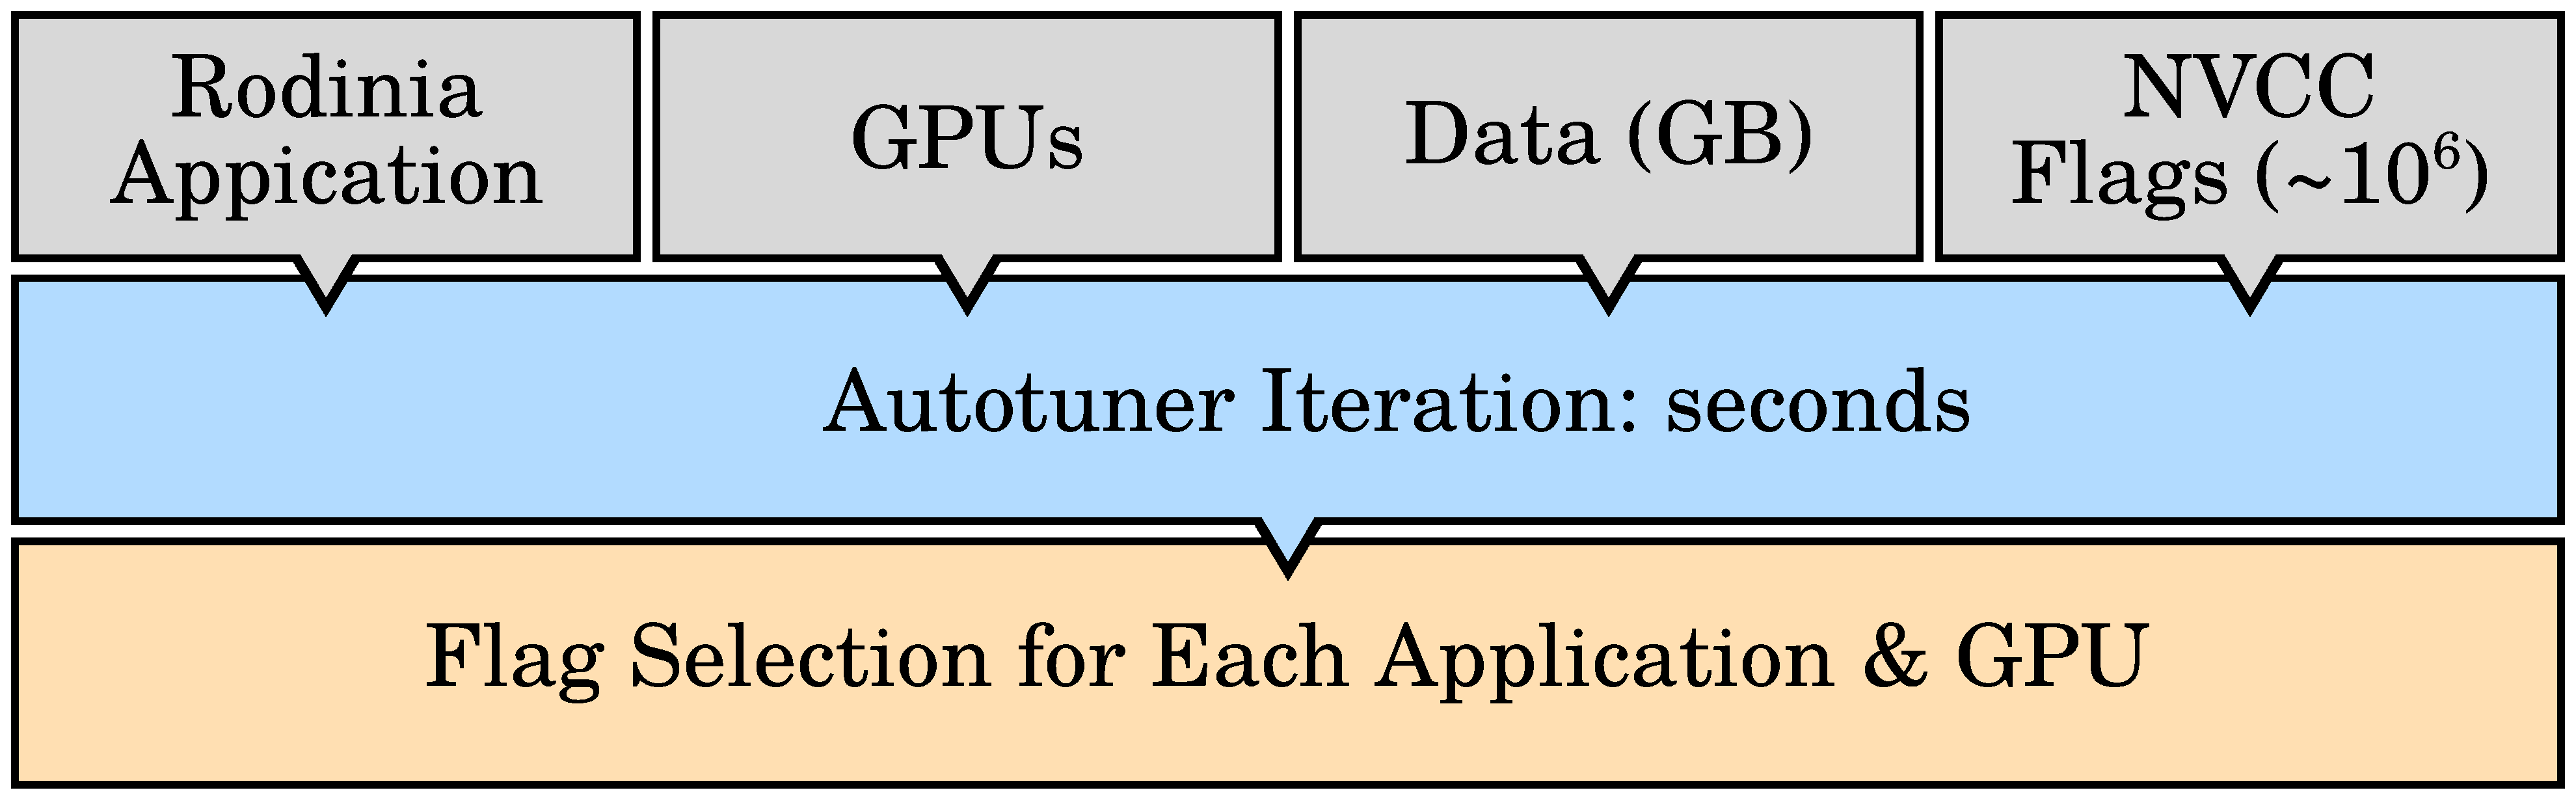
\includegraphics[width=.65\textwidth]{./images/overview_gpus}
    \caption{Autotuner Representation}
    \label{fig:overview-gpus}
\end{figure}

Figure~\ref{fig:overview-gpus} shows a representation of the autotuner
implemented in this study. The autotuner, in light blue, receives as input a
Rodinia application, a target GPU, input data for the application in the order
of Gigabytes and a search space composed of NVCC flags. The autotuner outputs
a flag selection subject to its input application and GPU.

Since in this study it was fast to compile and measure a program's performance,
an autotuner iteration is shown in Figure~\ref{fig:overview-gpus} to last in
the order of seconds. We could therefore test thousands of flag combinations
per hour in a sequential autotuner, exploring enough of the search space to
achieve the speedups reported.

The tool we used to implement our autotuner was not able to run measurements in
distributed environments. Therefore our autotuner could not deploy measurements
of different configurations on identical GPUs on the same network. An autotuner
with such capability would enable the exploration of more configurations in the
same time.

\subsection{A Tool for Compiler Autotuning}
\todo[inline,author=Pedro,color=cyan]{Describe our new NVCC autotuner presented
at the NVIDIA workshop. This could be left to the last chapter.}

\subsection{Background}

\subsubsection{NVIDIA GPU Microarchitecture}
\label{sec:GPUsCUDA}

NVIDIA GPU architectures have multiple asynchronous and parallel Streaming
Multiprocessors (SMs) which contain Scalar Processors (SPs), Special Function
Units (SFUs) and load/store units. Each group of 32 parallel threads scheduled
by and SM, or \textit{warp}, is able to read from memory concurrently.  The
Tesla, Fermi, Kepler and Maxwell NVIDIA architectures vary in a large number of
features, such as number of cores, registers, SFUs, load/store units, on-chip
and cache memory sizes, processor clock frequency, memory bandwidth, unified
memory spaces and dynamic kernel launches.  Those differences are summarized in
the Compute Capability (C.C.) of an NVIDIA GPU.

The hierarchical memory of an NVIDIA GPU contains global and shared portions.
Global memory is big, off-chip, has a high latency and can be accessed by all
threads of the kernel.  Shared memory is small, on-chip, has a low-latency and
can be accessed only by threads in a same SM.  Each SM has its own shared L1
cache, and new architectures have coherent global L2 caches.  Optimizing thread
accesses to different memory levels is essential to achieve good performance.

\subsubsection{Compute Unified Device Architecture (CUDA)}

The CUDA programming model and platform enables the use of NVIDIA GPUs for
scientific and general purpose computation.  A single \textit{master} thread
runs in the CPU, launching and managing computations on the GPU.  Data for the
computations has to be transferred from the main memory to the GPU's memory.
Multiple computations launched by the master thread, or \textit{kernels}, can
run asynchronously and concurrently. If the threads from a same warp must
execute different instructions the CUDA compiler must generate code to branch
the execution correctly, making the program lose performance due to this
\textit{warp divergence}.

The CUDA language extends C and provides a multi-step compiler, called
\textit{NVCC}, that translates CUDA code to Parallel Thread Execution code, or
\textit{PTX}.  \textit{NVCC} uses the host's C++ compiler in several
compilation steps, and also to generate code to be executed in the host. The
final binary generated by \textit{NVCC} contains code for the GPU and the host.
When \textit{PTX} code is loaded by an application at run-time, it is compiled
to binary code by the host's device driver.  This binary code can be executed
in the device's processing cores, and is architecture-specific.  The targeted
architecture can be specified using \textit{NVCC} parameters.

\subsubsection{GPU Performance Models and Autotuning}

The accuracy of a GPU performance model is subject to low level elements such
as instruction pipeline usage and small cache hierarchies. A GPU's performance
approaches its peak when the instruction pipeline is saturated, but becomes
unpredictable when the pipeline is
under-utilized~\cite{zhang2011quantitative,amaris2015simple}.  Considering the
effects of small cache hierarchies~\cite{dao2015performance,picchi2015impact}
and memory-access
divergence~\cite{sampaio2013divergence,baghsorkhi2010adaptive} is also critical
to a GPU performance model.

Guo and Wang~\cite{guo2010auto} introduce a framework for autotuning
the number of threads and the sizes of blocks and warps used by the CUDA
compiler for sparse matrix and vector multiplication GPU applications.  Li
\emph{et al.}~\cite{li2009note} discuss the performance of autotuning
techniques in highly-tuned GPU General Matrix to Matrix Multiplication (GEMMs)
routines, highlighting the difficulty in developing optimized code for new GPU
architectures.  Grauer-Gray \emph{et al.}~\cite{grauer2012auto}
autotune an optimization space of GPU kernels focusing on tiling, loop
permutation, unrolling, and parallelization.  Chaparala \emph{et
al.}~\cite{chaparala2015autotuning} autotune GPU-accelerated Quadratic
Assignment Problem solvers.  Sedaghati \emph{et
al.}~\cite{sedaghati2015automatic} build a decision model for the selection of
sparse matrix representations in GPUs.

\subsection{Autotuner \& Search Space}
\label{sec:tunersearch}

This section discusses our autotuner implementation and the
search space of NVCC compiler parameters.

\subsubsection{Autotuner}

The autotuner we implemented used the \textit{multi-armed bandit with sliding
window, area under the curve credit assignment} meta-technique, simply named
\textit{AUC Bandit}.  AUC Bandit is OpenTuner's core
meta-technique~\cite{ansel2014opentuner}, and its ensemble of search techniques
is composed by implementations of the Nelder-Mead algorithm and three
variations of genetic algorithms.  Figure~\ref{fig:gpu-stack} shows a
simplified version of the steps necessary to generate the object code that will
be measured later.

The code for our autotuner and all the experiments and results is
available\footnote{Hosted at GitHub:
\url{https://github.com/phrb/gpu-autotuning} [Accessed on 10 February 2015]}
under the GNU General Public License.

\begin{figure}[htpb]
    \centering
    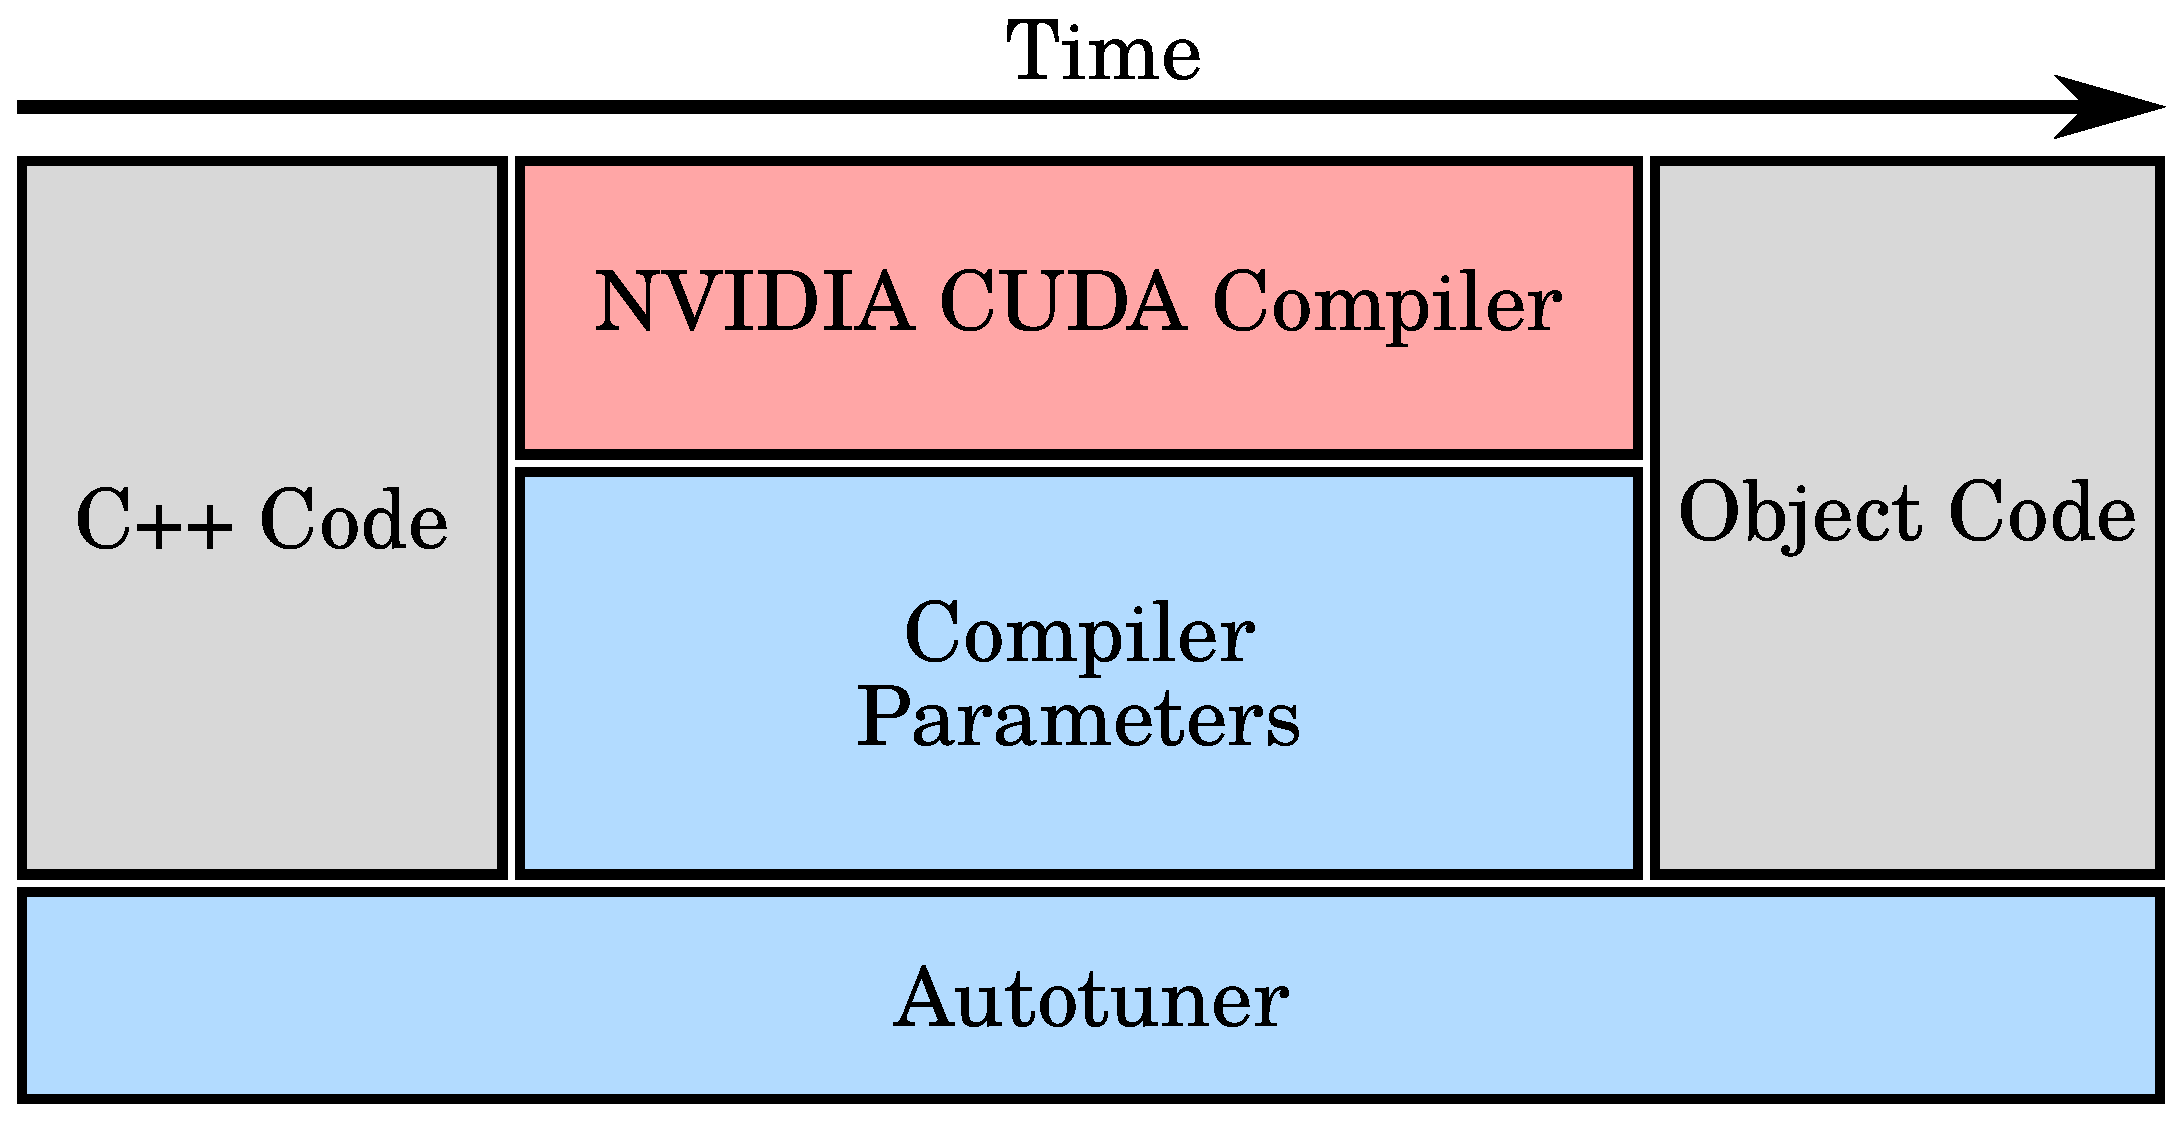
\includegraphics[width=.4\textwidth]{./images/gpu-stack}
    \caption{Simplified view of NVCC compilation}
    \label{fig:gpu-stack}
\end{figure}

\subsubsection{Search Space}

Table~\ref{tab:flags} details the subset of the CUDA configuration parameters
used in the experiments~\footnote{Adapted from:
\url{http://docs.nvidia.com/cuda/cuda-compiler-driver-nvcc} [Accessed on 10
February 2015]}.  The parameters target different compilation steps: the
\emph{PTX} optimizing assembler; the \emph{NVLINK} linker; and the \emph{NVCC}
compiler.  We compared the performance of programs generated by tuned
parameters with the standard compiler optimizations, namely
\texttt{--opt-level=0,1,2,3}.  Different \texttt{--opt-level}s could also be
selected during tuning.  We did not use compiler options that target the host
linker or the library manager since they do not affect performance.  The size
of the search space defined by all possible combinations of the flags in
Table~\ref{tab:flags} is in the order of $10^{6}$ making hand-optimization or
exhaustive searches very time consuming.

\begin{table}[htpb]
    \centering
    \tiny
        \begin{tabular}{lp{0.6\textwidth}}
        \toprule
        \textbf{Flag}&\textbf{Description} \\\midrule
        \texttt{no-align-double} & Specifies that \texttt{malign-double} should not be passed as a compiler argument on 32-bit platforms. \textbf{Step}: NVCC \\ \midrule
        \texttt{use\_fast\_math} & Uses the fast math library, implies \texttt{ftz=true}, \texttt{prec-div=false}, \texttt{prec-sqrt=false} and \texttt{fmad=true}. \textbf{Step}: NVCC \\\midrule
        \texttt{gpu-architecture} & Specifies the NVIDIA virtual GPU architecture for which the CUDA input files must be compiled. \textbf{Step}: NVCC \textbf{Values}: \texttt{sm\_20}, \texttt{sm\_21}, \texttt{sm\_30}, \texttt{sm\_32}, \texttt{sm\_35}, \texttt{sm\_50}, \texttt{sm\_52} \\\midrule
        \texttt{relocatable-device-code} & Enables the generation of relocatable device code. If disabled, executable device code is generated. Relocatable device code must be linked before it can be executed. \textbf{Step}: NVCC \\\midrule
        \texttt{ftz} & Controls single-precision denormals support. \texttt{ftz=true} flushes denormal values to zero and \texttt{ftz=false} preserves denormal values. \textbf{Step}: NVCC \\\midrule
        \texttt{prec-div} & Controls single-precision floating-point division and reciprocals. \texttt{prec-div=true} enables the IEEE round-to-nearest mode and \texttt{prec-div=false} enables the fast approximation mode. \textbf{Step}: NVCC \\\midrule
        \texttt{prec-sqrt} & Controls single-precision floating-point squre root. \texttt{prec-sqrt=true} enables the IEEE round-to-nearest mode and \texttt{prec-sqrt=false} enables the fast approximation mode. \textbf{Step}: NVCC \\\midrule
        \texttt{def-load-cache} & Default cache modifier on global/generic load. \textbf{Step}: PTX \textbf{Values}: \texttt{ca}, \texttt{cg}, \texttt{cv}, \texttt{cs} \\\midrule
        \texttt{opt-level} & Specifies high-level optimizations. \textbf{Step}: PTX \textbf{Values}: \texttt{0 - 3} \\\midrule
        \texttt{fmad} & Enables the contraction of floating-point multiplies and adds/subtracts into floating-point multiply-add operations (FMAD, FFMA, or DFMA). \textbf{Step}: PTX \\\midrule
        \texttt{allow-expensive-optimizations} & Enables the compiler to perform expensive optimizations using maximum available resources (memory and compile-time). If unspecified, default behavior is to enable this feature for optimization level $\geqslant$O2. \textbf{Step}: PTX \\\midrule
        \texttt{maxrregcount} & Specifies the maximum number of registers that GPU functions can use. \textbf{Step}: PTX \textbf{Values}: \texttt{16 - 64} \\\midrule
        \texttt{preserve-relocs} & Makes the \texttt{PTX} assembler generate relocatable references for variables and preserve relocations generated for them in the linked executable. \textbf{Step}: NVLINK \\\midrule
        \end{tabular}
    \caption{Description of flags in the search space}
    \label{tab:flags}
\end{table}

\subsection{Experiments}

This section presents the GPU testbed, the algorithm benchmark, the
autotuner implementation and its search space.

\subsubsection{GPU Testbed}

To be able to show that different GPUs require different options to improve
performance, and that it is possible to achieve speedups in different hardware,
we wanted to tune our benchmark for different NVIDIA microarchitectures.
Table~\ref{tab:GPUs} summarizes the hardware characteristics of the three GPUs.

\begin{table}[thpb]
    \centering
    \footnotesize
    \begin{tabular}{cccccccc}
        \toprule
        \textbf{Model}&\textbf{C.C.}&\textbf{Global Memory}&\textbf{Bus}&\textbf{Bandwidth}&\textbf{L2}&\textbf{Cores/SM}&\textbf{Clock} \\ \midrule
        Tesla-K40&3.5&12 GB&384-bit&276.5 GB/s&1.5 MB&2880/15&745 Mhz \\ \midrule
        GTX-750&5.0&1 GB&128-bit&86.4 GB/s&2 MB&512/4&1110 Mhz \\ \midrule
        GTX-980&5.2&4 GB&256-bit&224.3 GB/s&2 MB&2048/16&1216 Mhz \\ \bottomrule
    \end{tabular}
    \caption{Hardware specifications of the GPUs in the testbed}
    \label{tab:GPUs}
\end{table}

\subsubsection{Algorithm Benchmark}

We composed a benchmark with 17 heterogeneous GPU applications.  The benchmark
contains 4 optimization strategies for \emph{matrix multiplication} (counted as
a single application), 1 vector addition problem, 1 solution for the
\emph{maximum sub-array problem}~\cite{ferreira2014parallel}, 2 \emph{sorting}
algorithms and 12 applications from the Rodinia Benchmark
Suite~\cite{che2009rodinia}.

Table~\ref{tab:Rodinia} shows the Rodinia applications contained in our
benchmark and their correspondent three-letter code.  The other applications in
the benchmark were CUDA implementations of the following:

\begin{itemize}
    \item Matrix multiplications using:
        \begin{itemize}
             \item Global memory with non-coalesced accesses (MMU)
             \item Global memory with coalesced accesses (MMG)
             \item Shared memory with non-coalesced accesses to global memory
                 (MSU)
             \item Shared memory with coalesced accesses to global memory (MMS)
        \end{itemize}
    \item Simple vector addition algorithm (VAD)
    \item Solution~\cite{alves2004bsp,ferreira2014parallel} for the Maximum
        Sub-Array Problem (MSA)
    \item Quicksort (QKS) and Bitonicsort (BTN)~\footnote{Obtained from:
        \url{http://digitalcommons.providence.edu/student\_scholarship/7/}
        [Accessed on 10 February 2015]}
\end{itemize}

\begin{table}[htpb]
    \centering
    \footnotesize
        \begin{tabular}{lll}
            \toprule
            \textbf{Application} & \textbf{Berkeley Dwarf\cite{asanovic2009view}} & \textbf{Domain} \\\midrule
            B+Tree (BPT) & Graph Traversal& Search \\\midrule
            Back Propagation (BCK) & Unstructured Grid & Pattern Recognition \\\midrule
            Breadth-First Search (BFS) & Graph Traversal & Graph Algorithms \\\midrule
            Gaussian Elimination (GAU) & Dense Linear Algebra & Linear Algebra \\\midrule
            Heart Wall (HWL) & Structured Grid & Medical Imaging \\\midrule
            Hot Spot (HOT) & Structured Grid & Physics Simulation \\\midrule
            K-Means (KMN) & Dense Linear Algebra & Data Mining \\\midrule
            LavaMD (LMD) & N-Body & Molecular Dynamics \\\midrule
            LU Decomposition (LUD) & Dense Linear Algebra & Linear Algebra \\\midrule
            Myocyte (MYO) & Structured Grid & Biological Simulation \\\midrule
            Needleman-Wunsch (NDL) & Dynamic Programming & Bioinformatics \\\midrule
            Path Finder (PTF) & Dynamic Programming & Grid Traversal \\\bottomrule
        \end{tabular}
    \caption{Rodinia applications used in the experiments}
    \label{tab:Rodinia}
\end{table}

\subsection{Results}
\label{sec:GPUresults}

This section presents the speedups achieved for all algorithms in the
application benchmark, highlights the most significant speedups, and discusses
the performance and accuracy of the autotuner.

\subsubsection{Performance Improvements}

All boxplots presented in this section were made using the standard
implementations available for the R language.  The black band inside the boxes
represents the median of the measurements. The lower and upper bounds of the
box represent, respectively, the first and third quartiles of the data. The
whiskers represent the third and first quartile plus and minus the \emph{inner
quartile range} times 1.5. Finally, the circles represent the outliers.

Figures~\ref{fig:K40hwl}, \ref{fig:980gau}, \ref{fig:K40ptf} and
\ref{fig:K40myo} compare the distributions of 10 perfomance measurements of
binaries compiled with high-level compiler optimizations and with autotuned
compiler options. The results for the high-level optimizations
\texttt{--opt-level=0,1,2,3} were denoted by \emph{-O0}, \emph{-O1}, \emph{-O2}
and \emph{-O3}.  The results for the autotuned configurations were denoted by
the keyword \emph{Tuned}.

\begin{figure}[htpb]
    \centering
    \begin{minipage}{.48\textwidth}
        \centering
        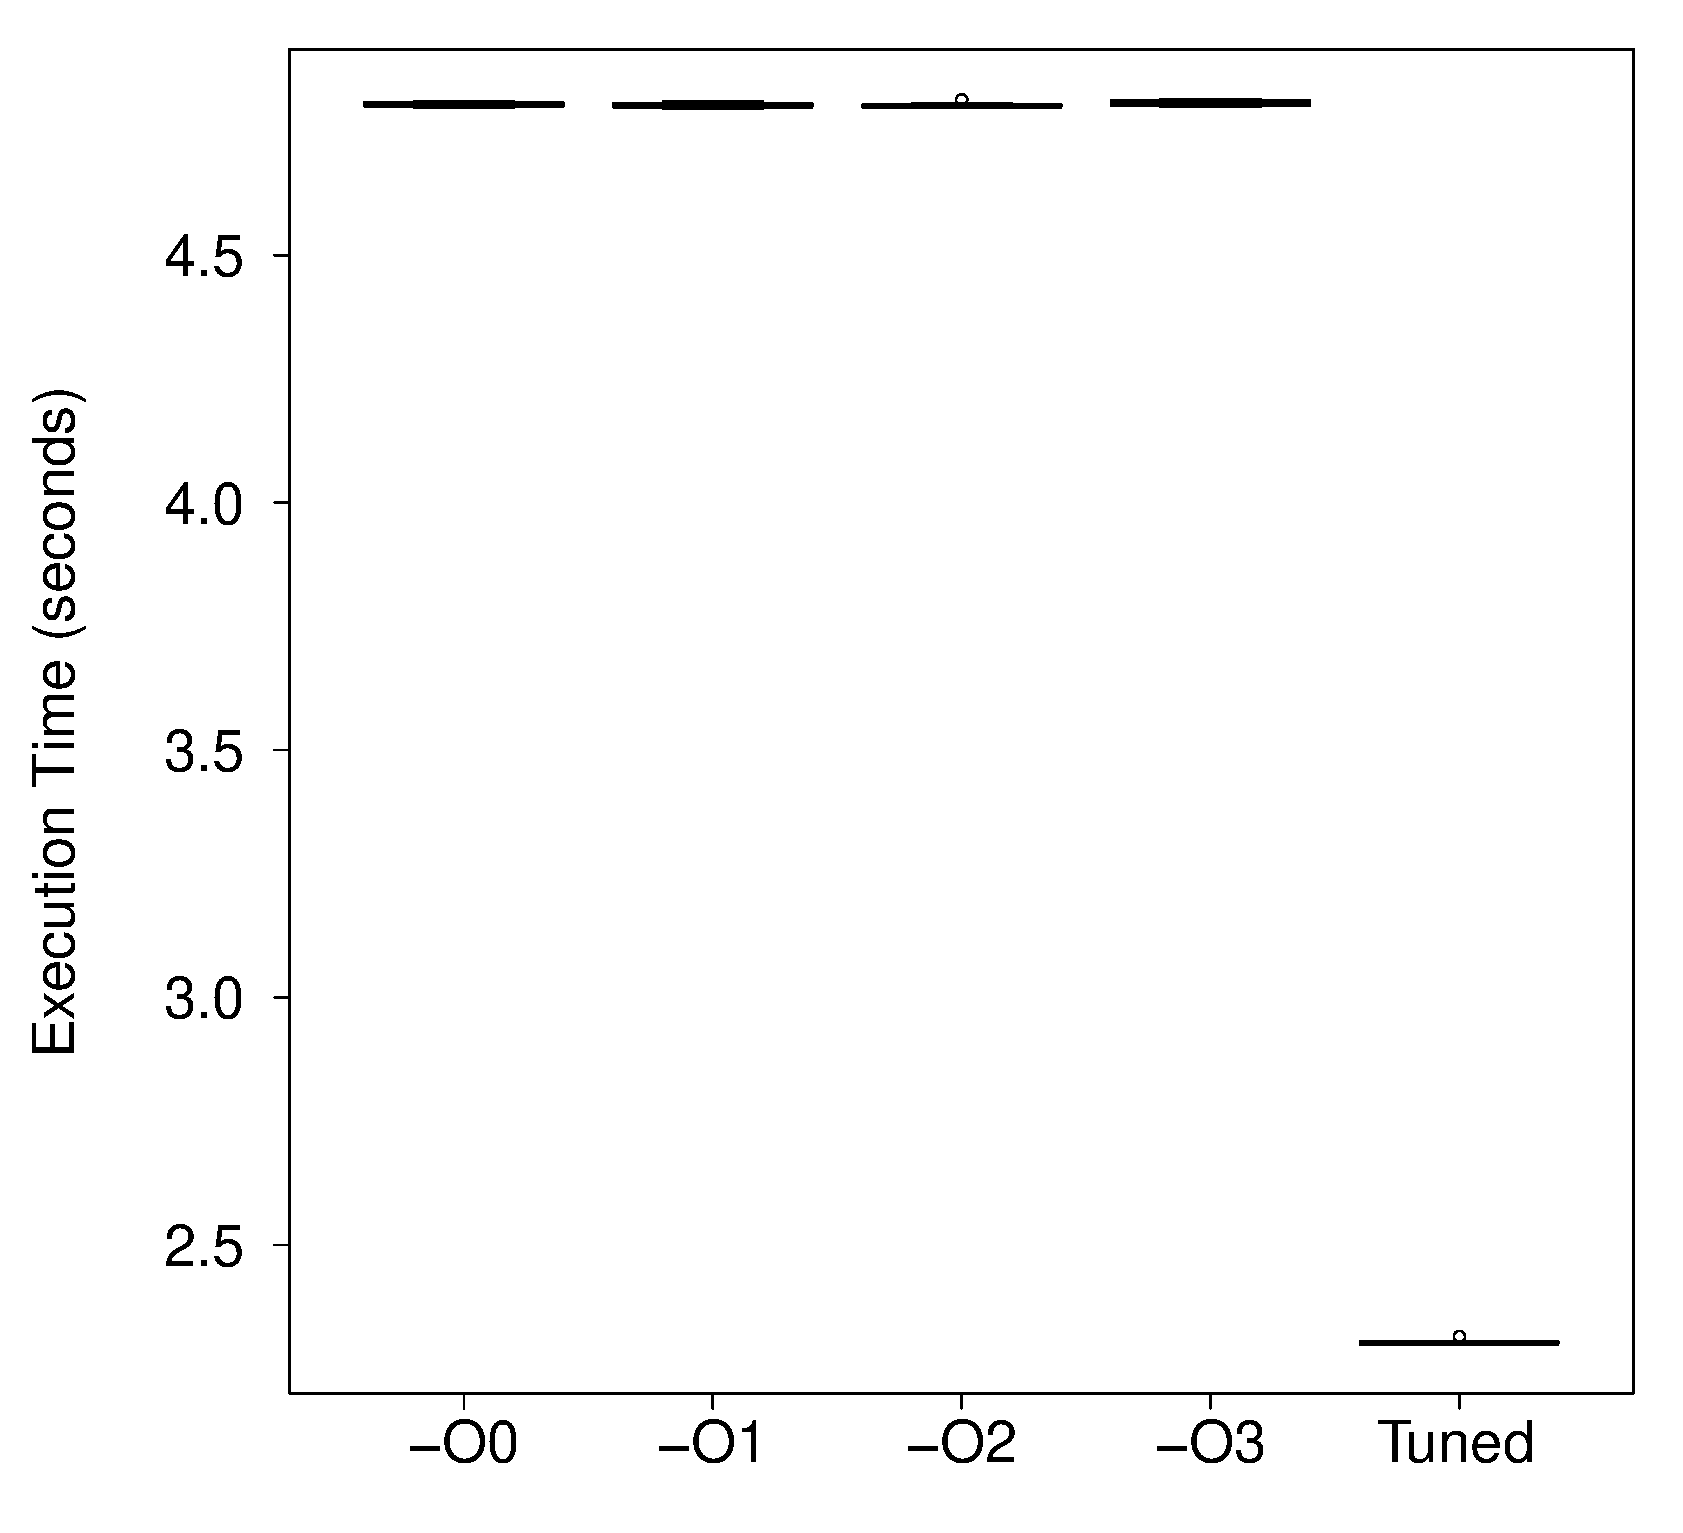
\includegraphics[scale=.22]{./images/heartwall-0-Tesla-K40-Box.eps}
        \caption{Boxplots for the Tesla K40, comparing autotuned results and high-level compiler optimizations for the Heart Wall problem (HWL)}
        \label{fig:K40hwl}
    \end{minipage}%
    \hfill
    \begin{minipage}{.48\textwidth}
        \centering
        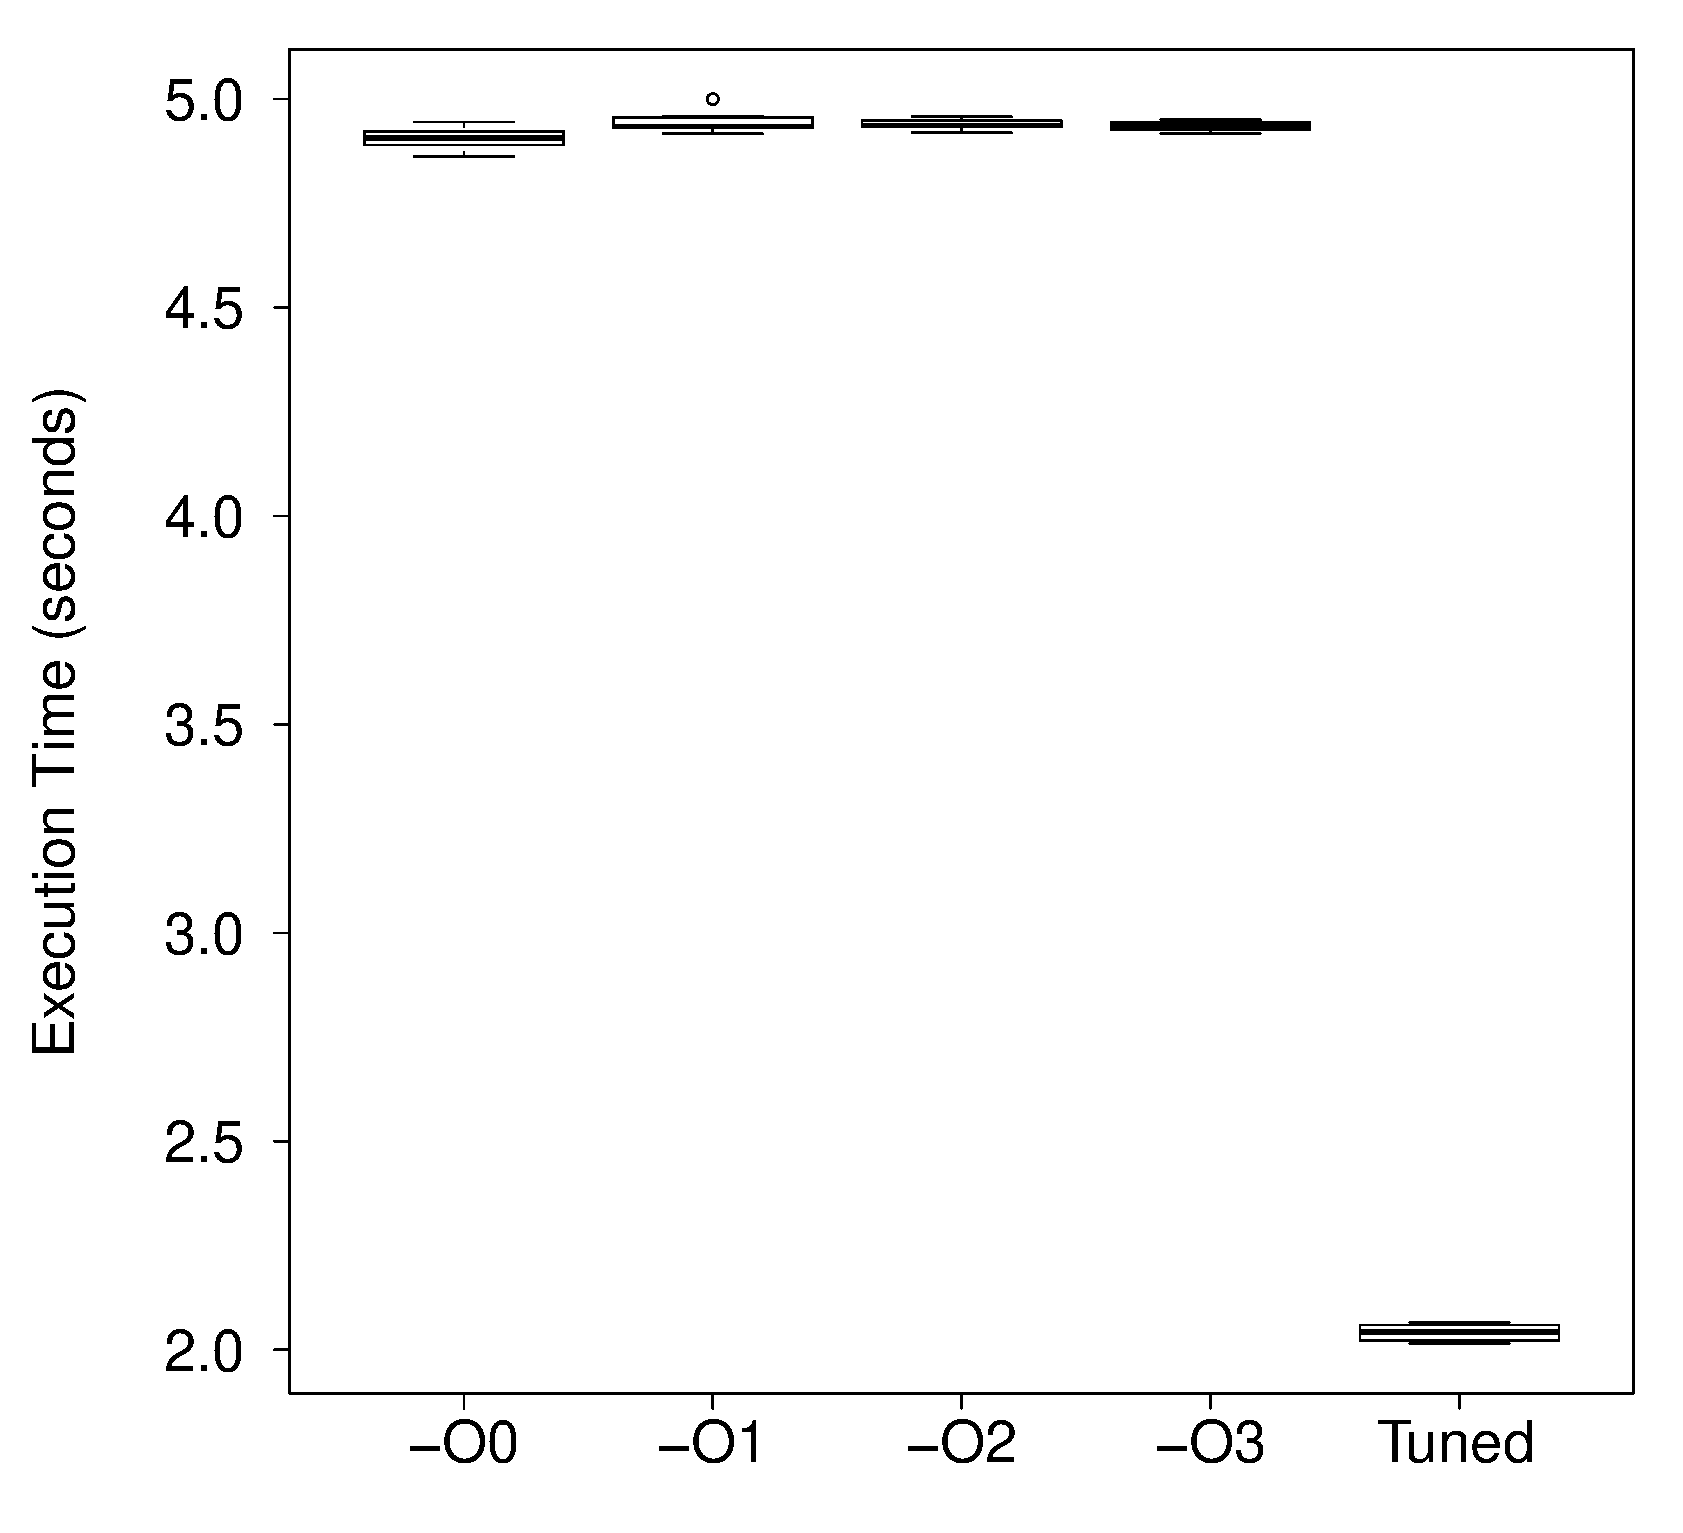
\includegraphics[scale=.22]{./images/gaussian-0-GTX-980-Box.eps}
        \caption{Boxplots for the GTX 980 GPU, comparing autotuned results and high-level compiler optimizations for the Gaussian Elimination problem (GAU)}
        \label{fig:980gau}
    \end{minipage}%

    \begin{minipage}{.48\textwidth}
        \centering
        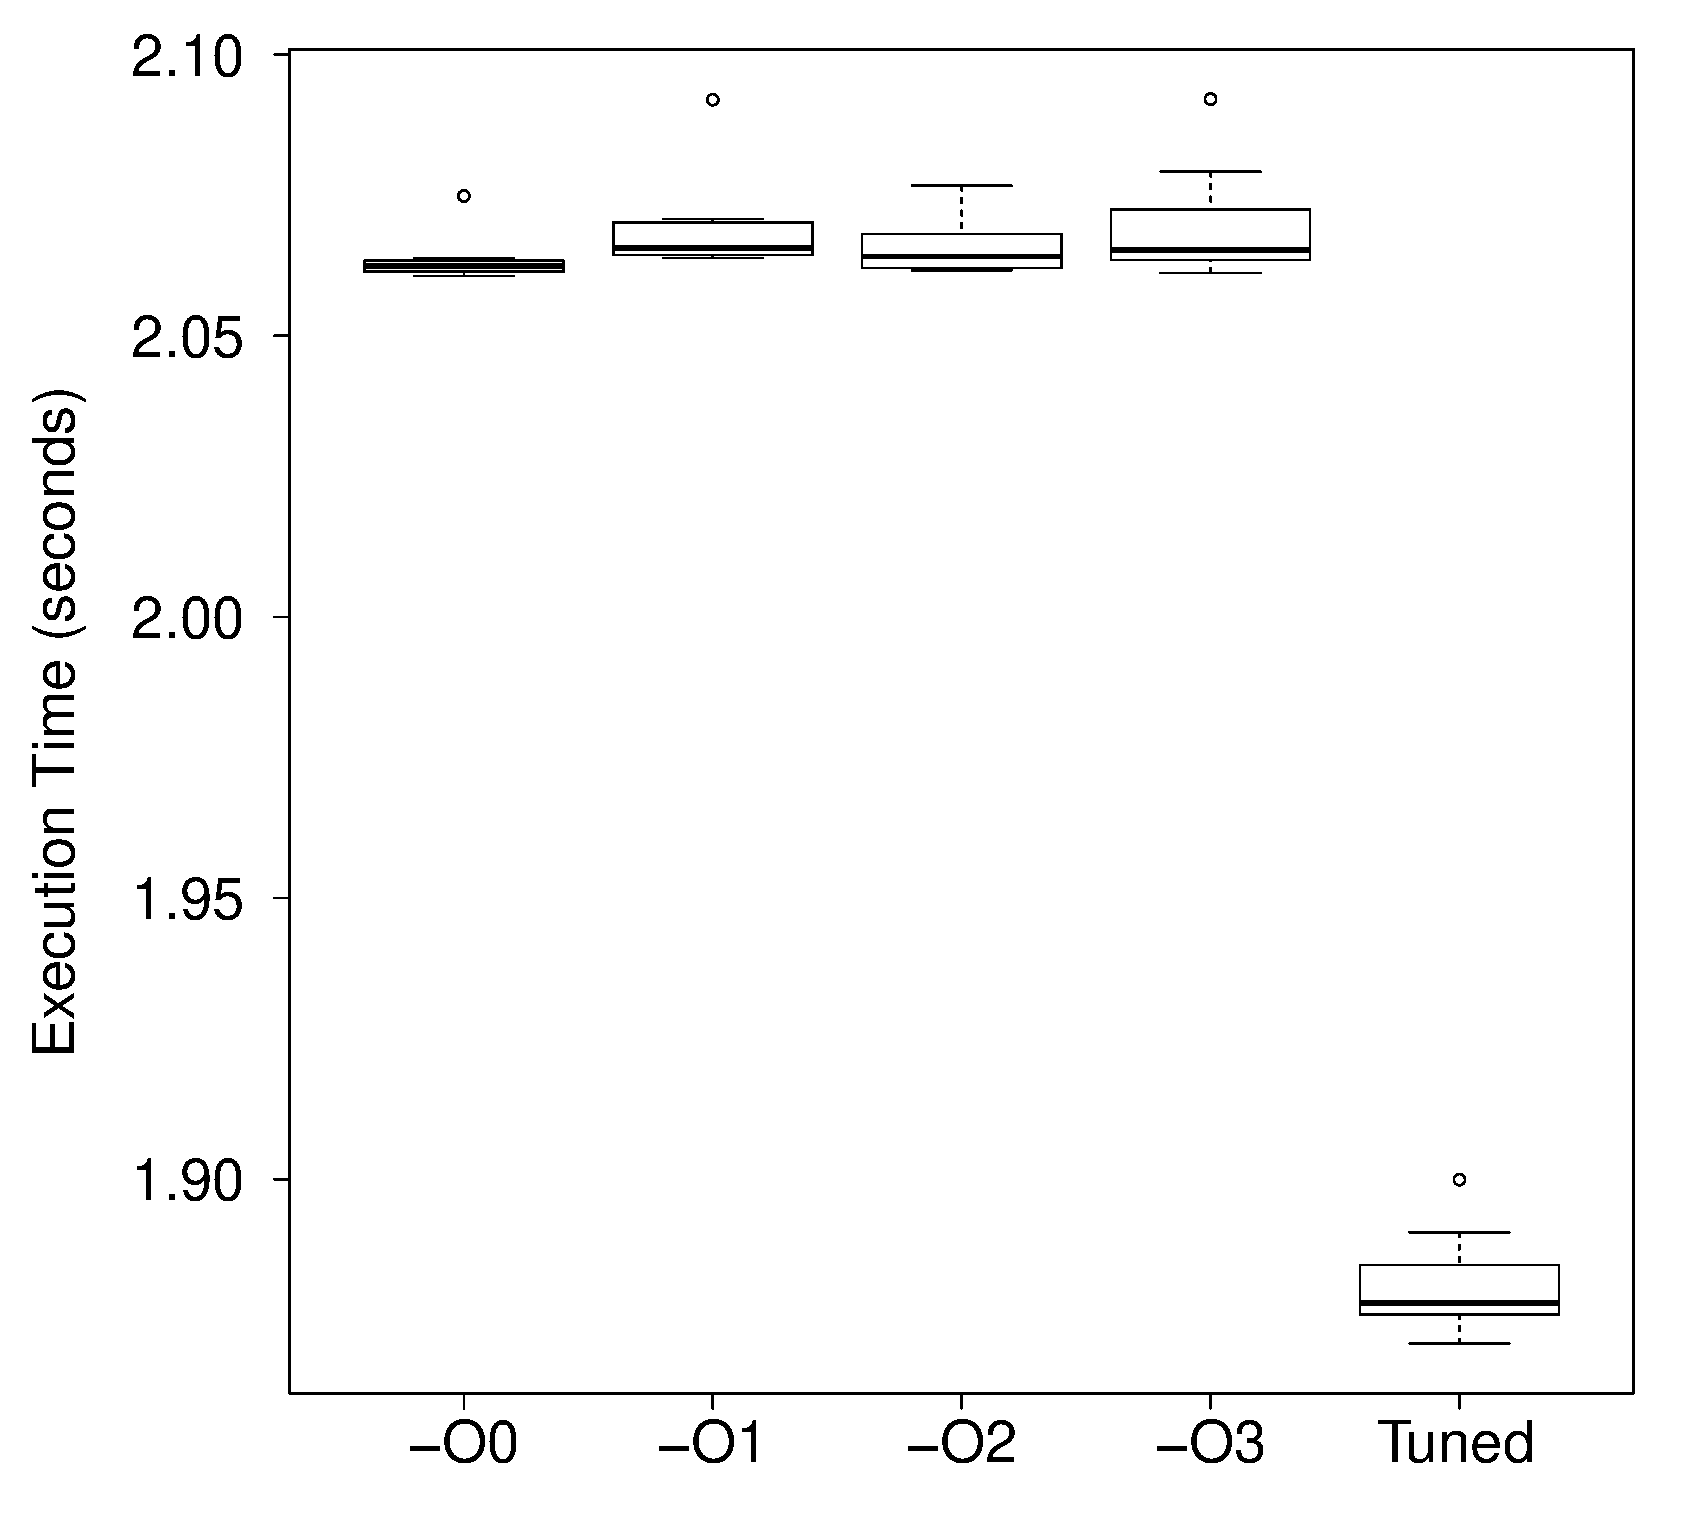
\includegraphics[scale=.22]{./images/Pathfinder-0-Tesla-K40-Box.eps}
        \caption{Boxplots for the Tesla K40, comparing autotuned results and high-level compiler optimizations for the Path Finder problem (PTF)}
        \label{fig:K40ptf}
    \end{minipage}%
    \hfill
    \begin{minipage}{.48\textwidth}
        \centering
        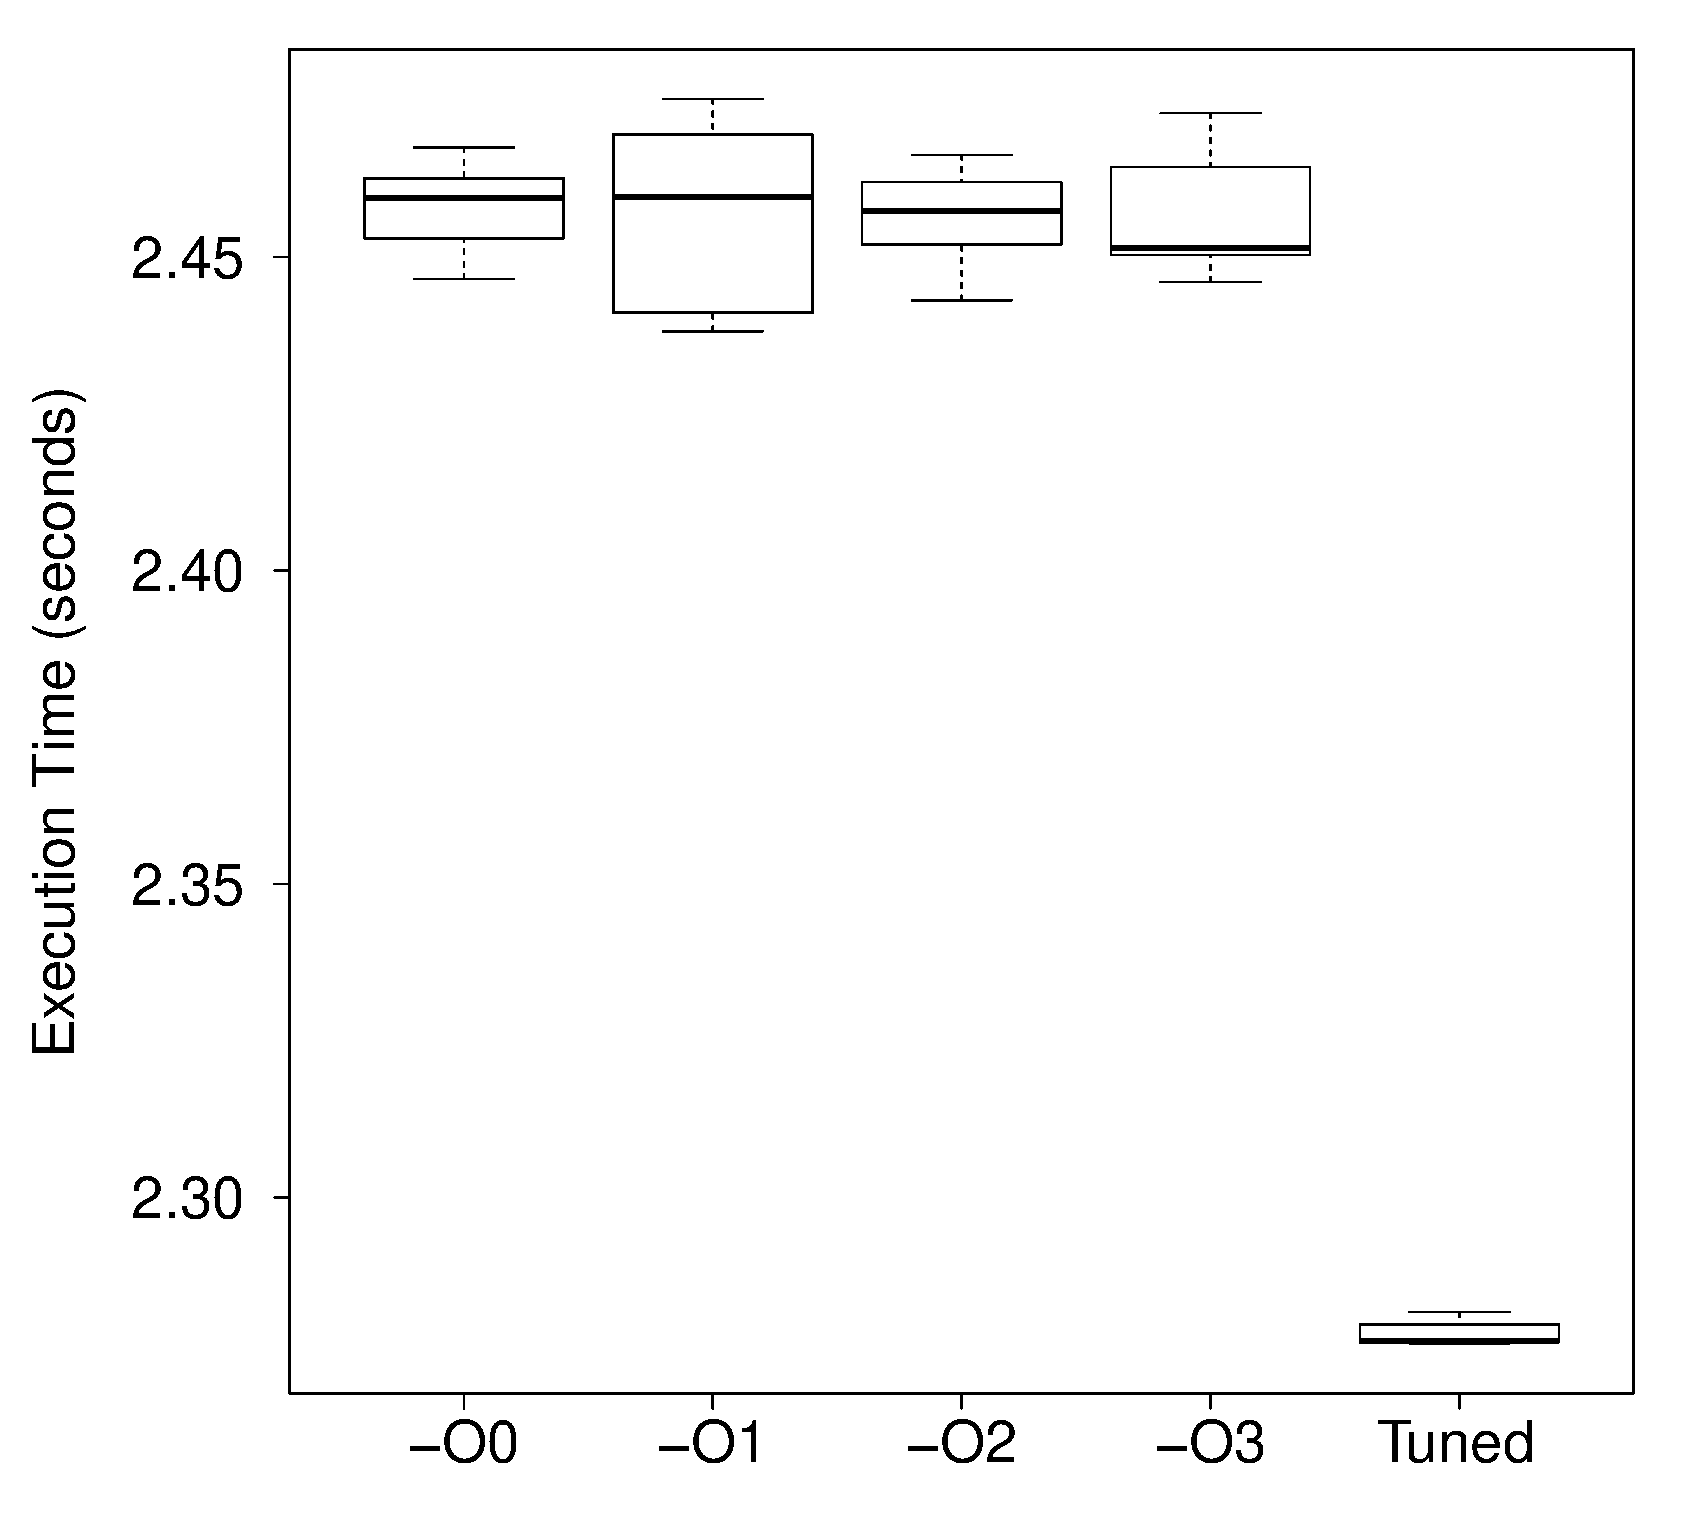
\includegraphics[scale=.22]{./images/myocyte-0-Tesla-K40-Box.eps}
        \caption{Boxplots for the Tesla K40, comparing autotuned results and high-level compiler optimizations for the Myocyte problem (MYO)}
        \label{fig:K40myo}
    \end{minipage}%
\end{figure}

Figure~\ref{fig:K40hwl} shows that the autotuned solution for the Heart Wall
problem (HWL) in the Tesla K40 achieved over 2x speedup in comparison with the
high-level CUDA optimizations.  Figure~\ref{fig:980gau} shows, in the GTX 980,
almost 2.5x speedup for the Gaussian Elimination problem (GAU).
Figure~\ref{fig:K40ptf} show 10\% speedup of the autotuned solution for the
Path Finder problem (PTF) in the Tesla K40.  Figure~\ref{fig:K40myo} shows over
5\% speedup of the autotuned solution, also in the Tesla K40, for the Myocyte
problem (MYO).

Figures~\ref{fig:matrixsummary}, \ref{fig:summary}, \ref{fig:rodiniasummary}
and \ref{fig:rodiniasummarysmall} present summaries of the results. The
autotuner did not find solutions that improved upon the high-level
optimizations for the problems BTN and MSU in any of the GPUs of the testbed,
but it found solutions that achieved speedups for at least one GPU for the
other problems.

\begin{figure}[htpb]
    \centering
    \begin{minipage}{.48\textwidth}
        \centering
        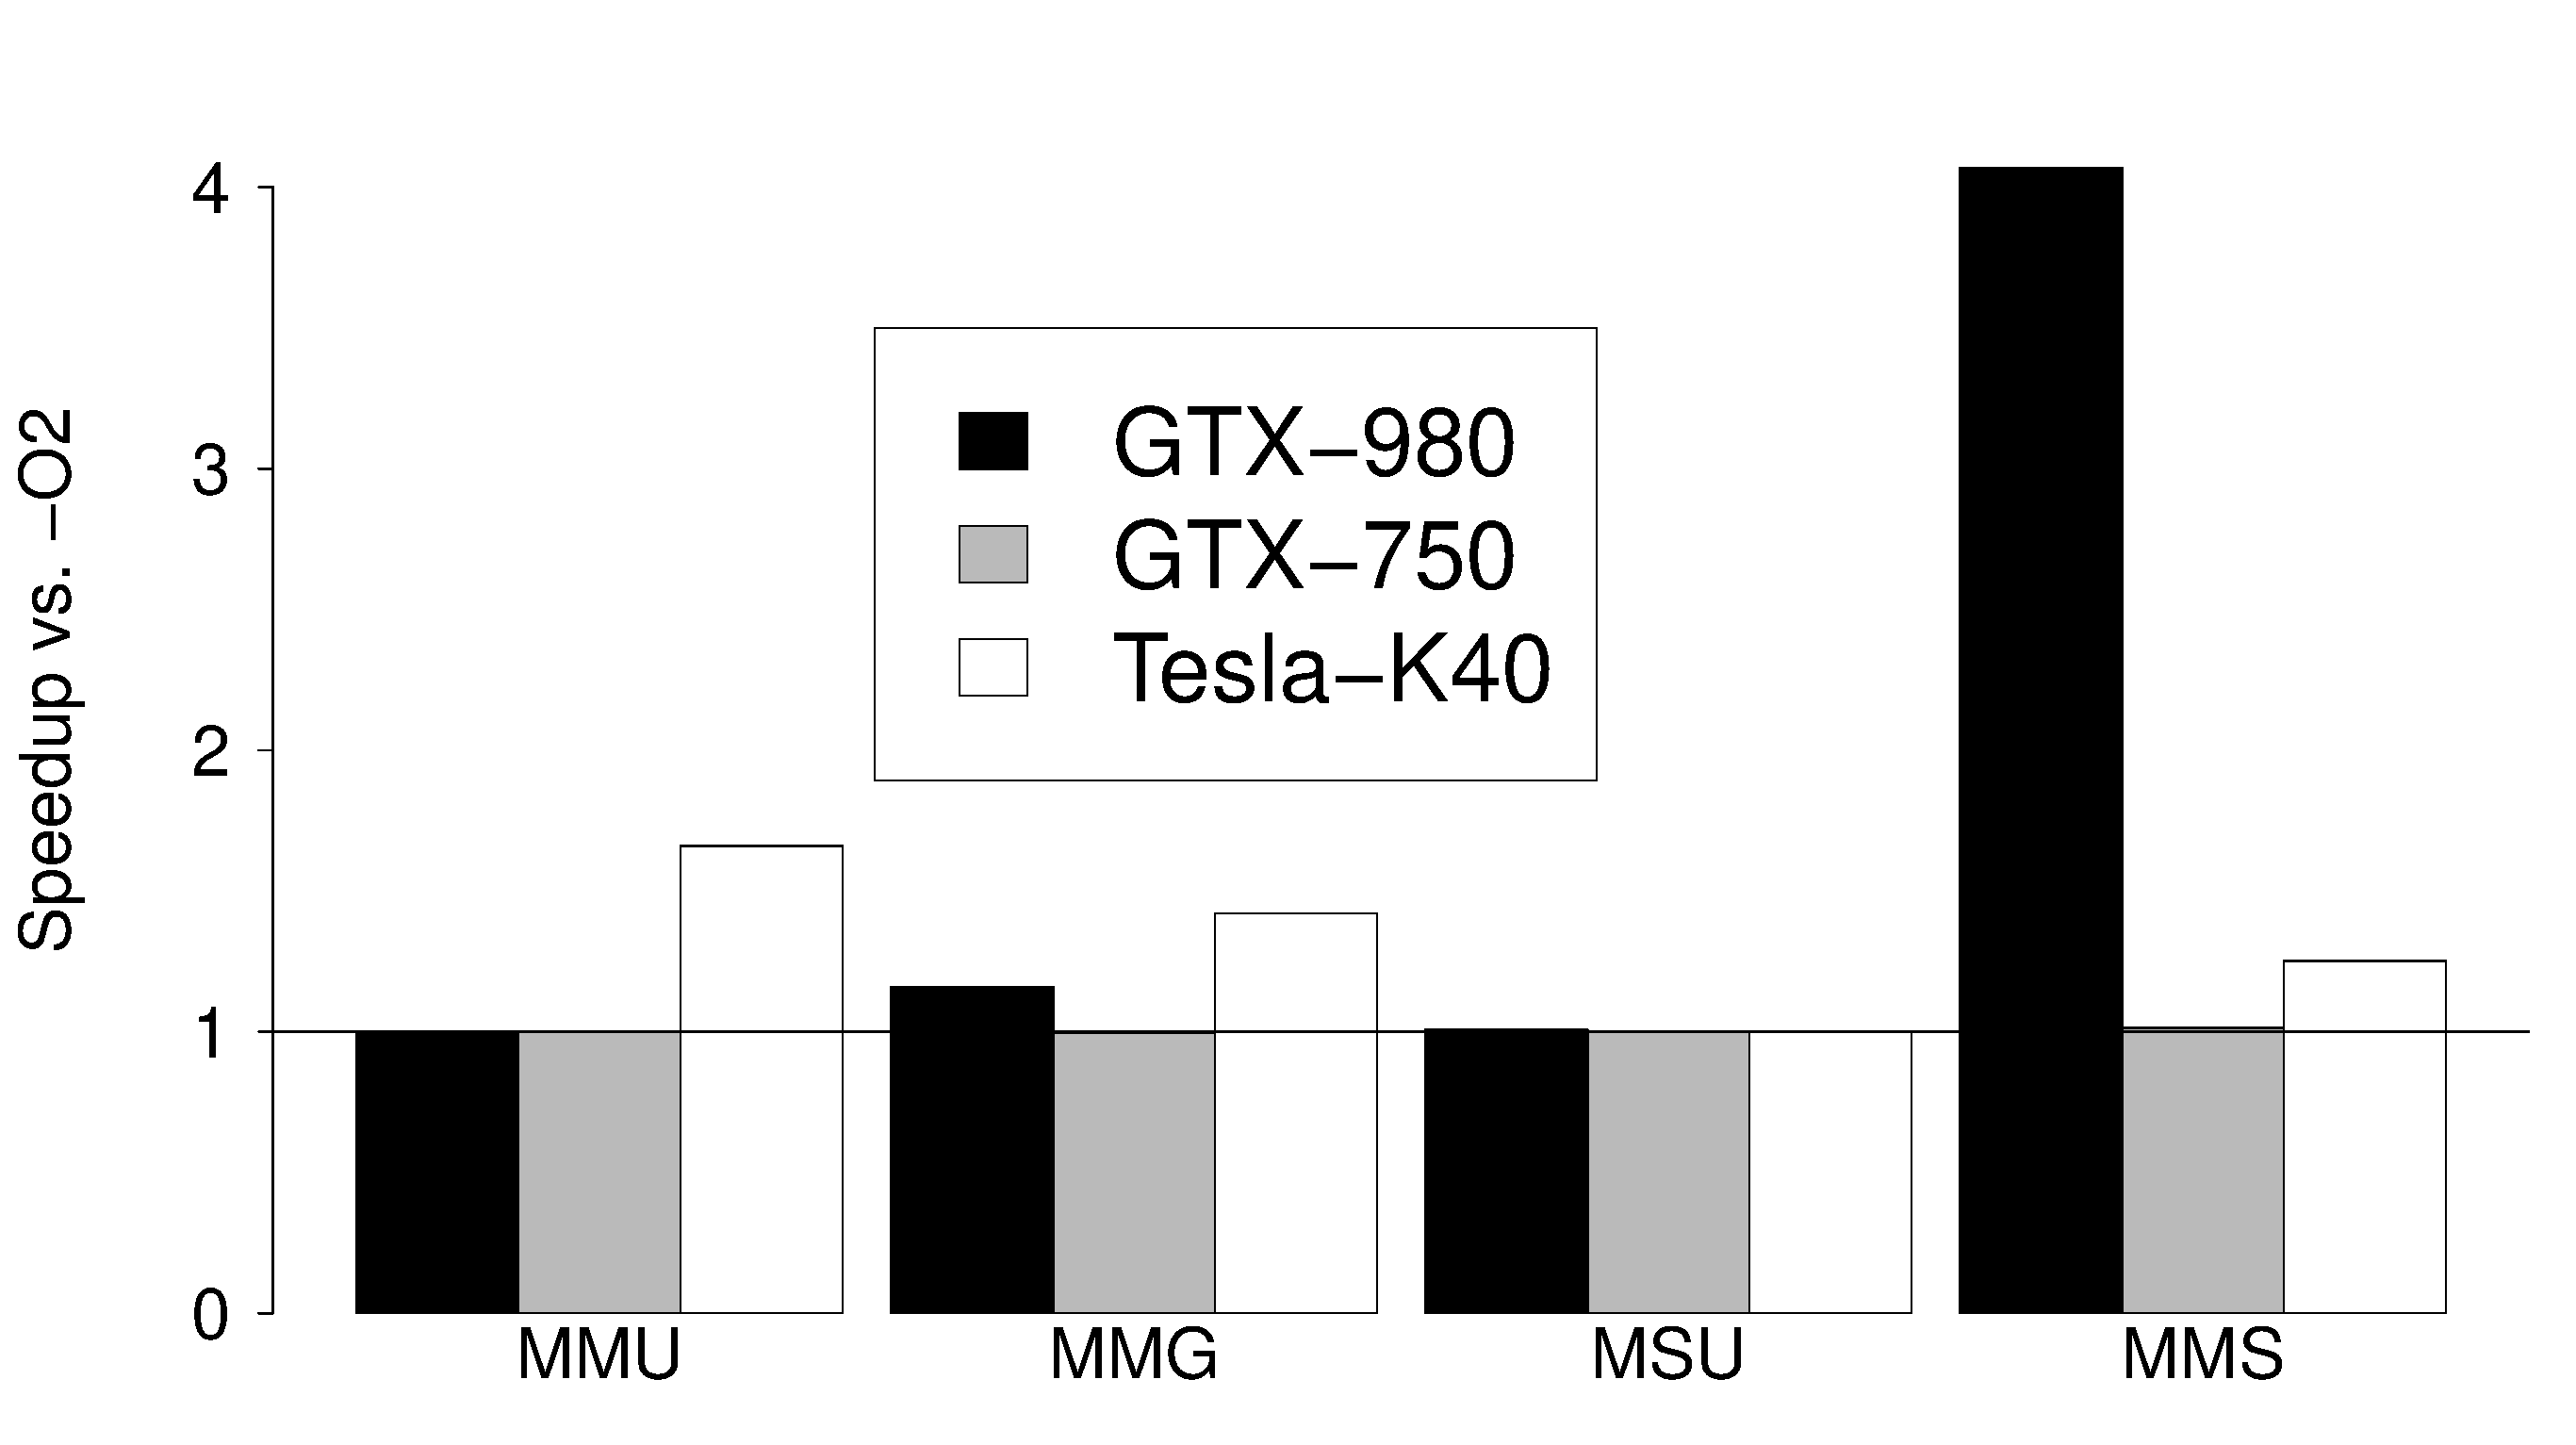
\includegraphics[scale=.15]{./images/MatrixSummary.eps}
        \caption{Summary of the speedups achieved versus \emph{-O2} in the matrix multiplication optimizations}
        \label{fig:matrixsummary}
    \end{minipage}%
    \hfill
    \begin{minipage}{.48\textwidth}
        \centering
        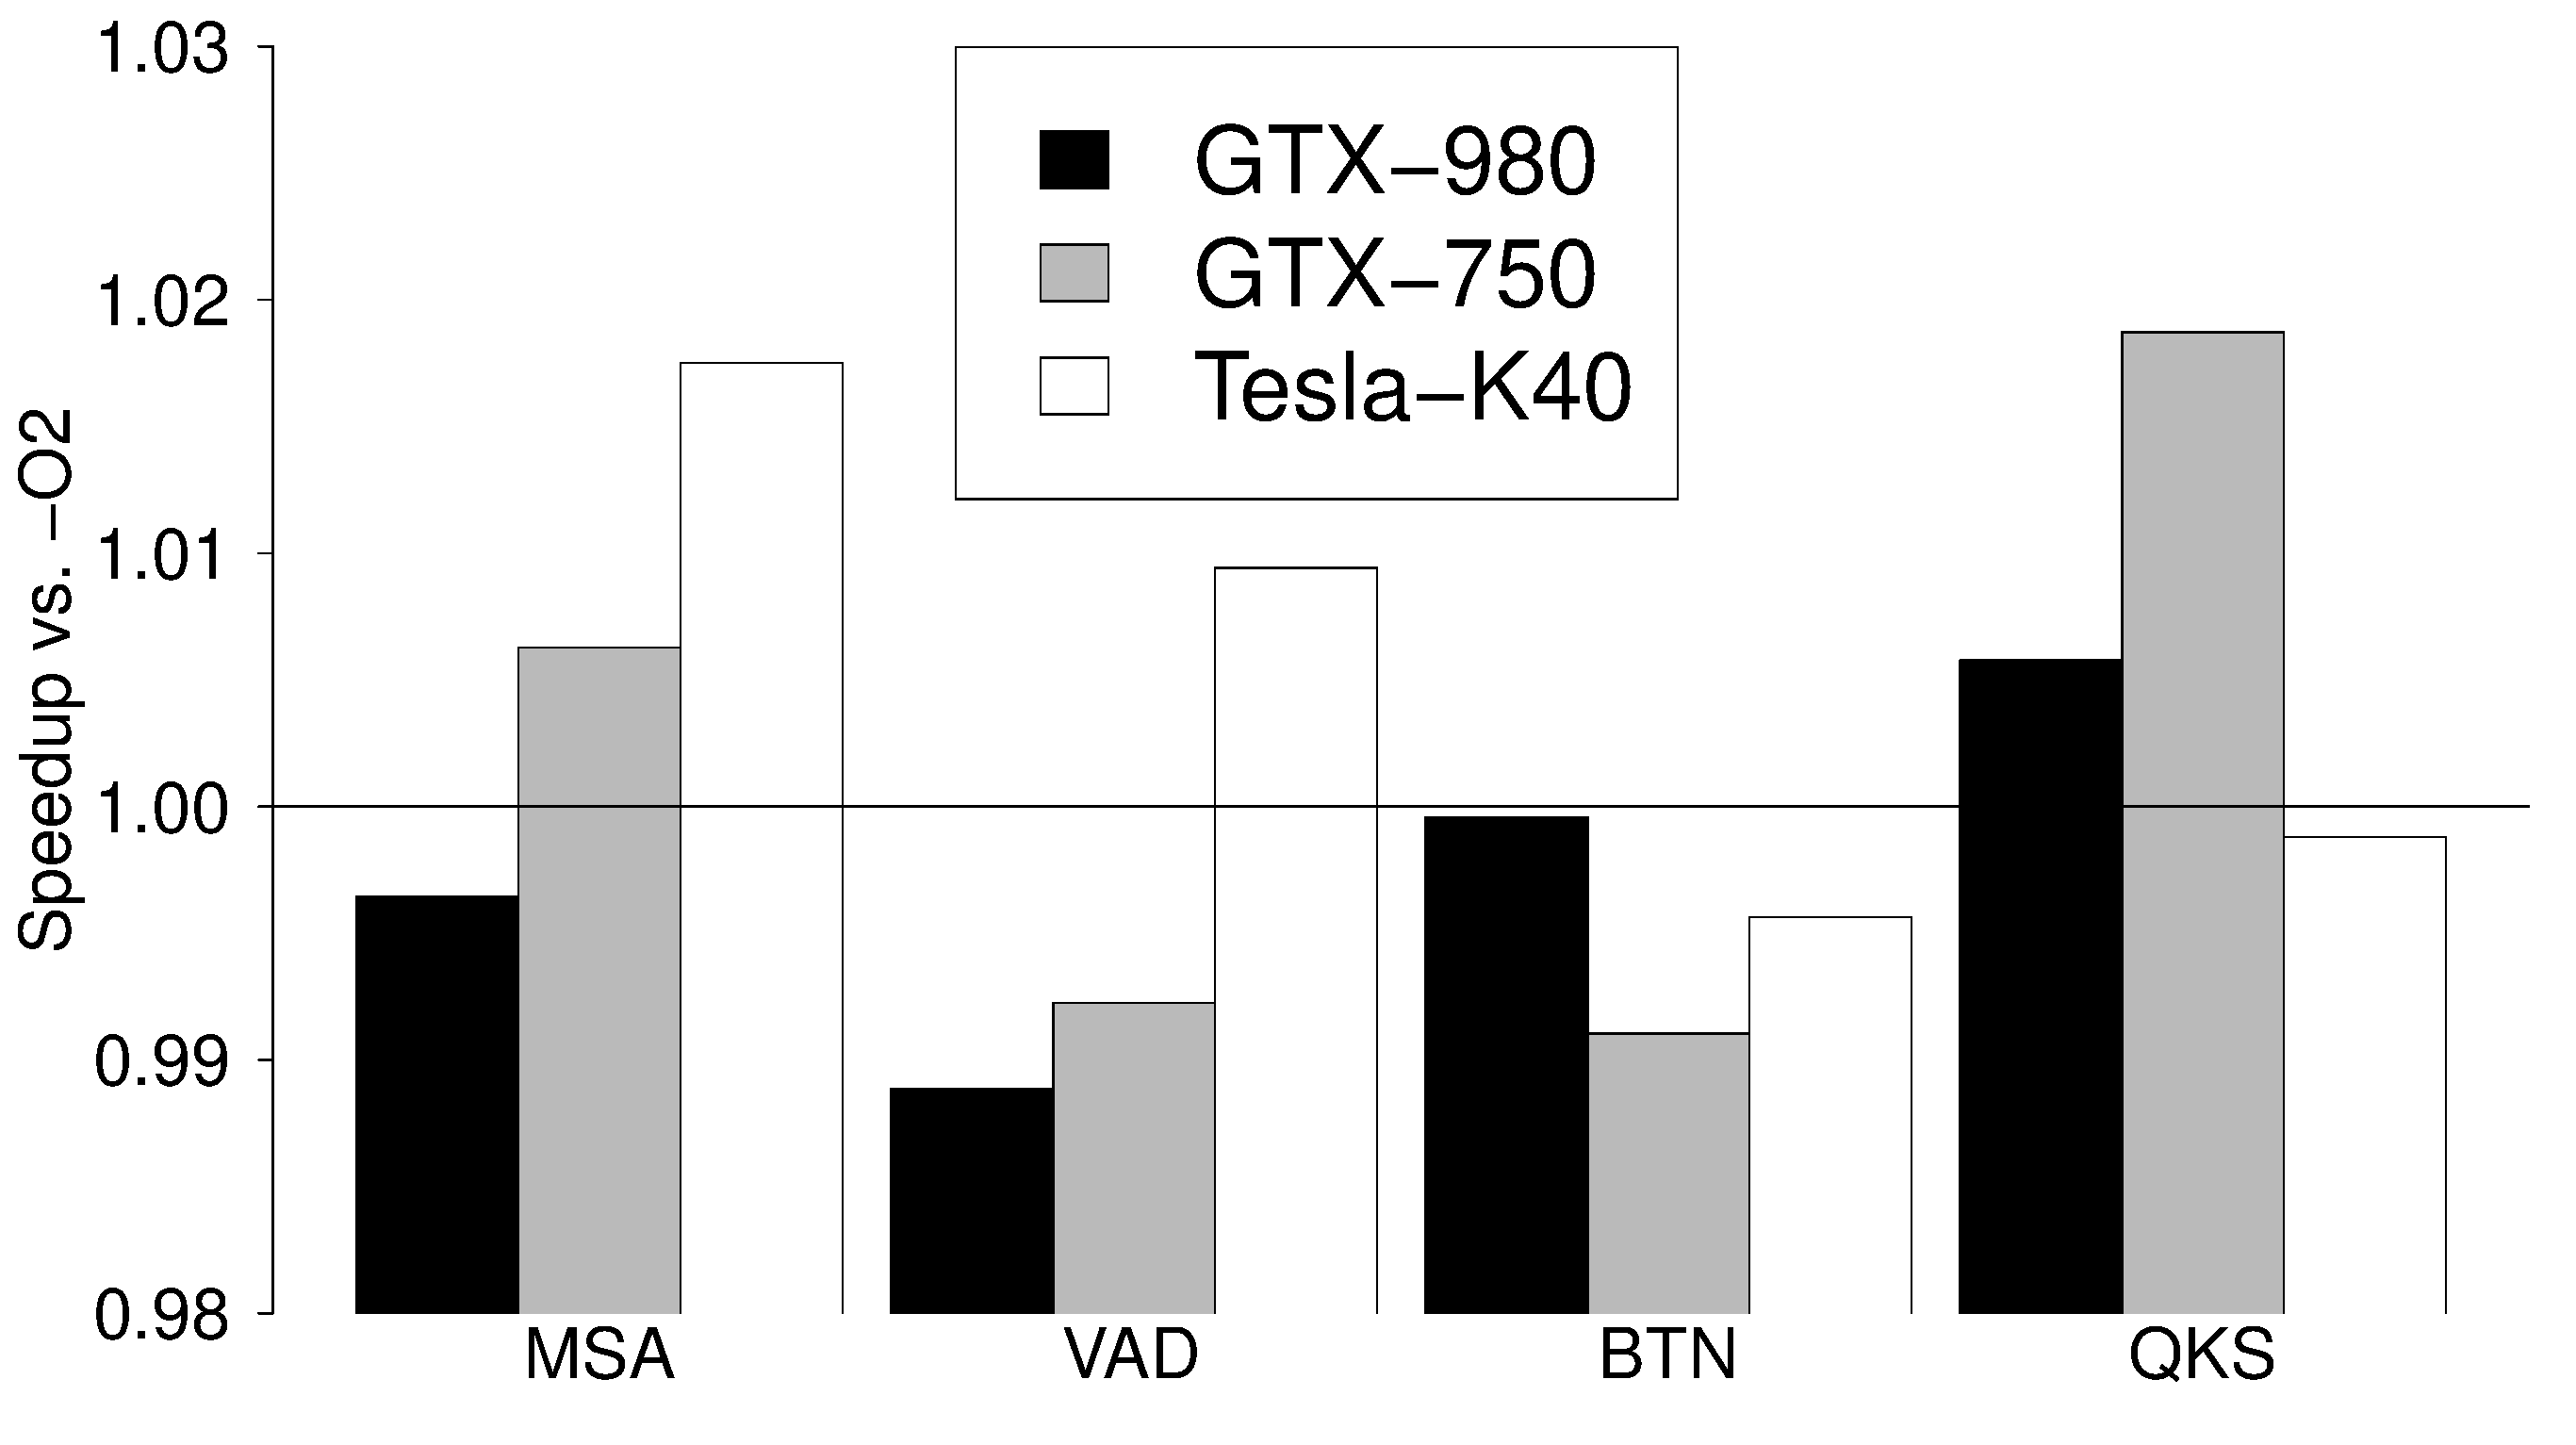
\includegraphics[scale=.15]{./images/Summary.eps}
        \caption{Summary of the speedups achieved versus \emph{-O2} in the other independent applications}
        \label{fig:summary}
    \end{minipage}%

    \begin{minipage}{.48\textwidth}
        \centering
        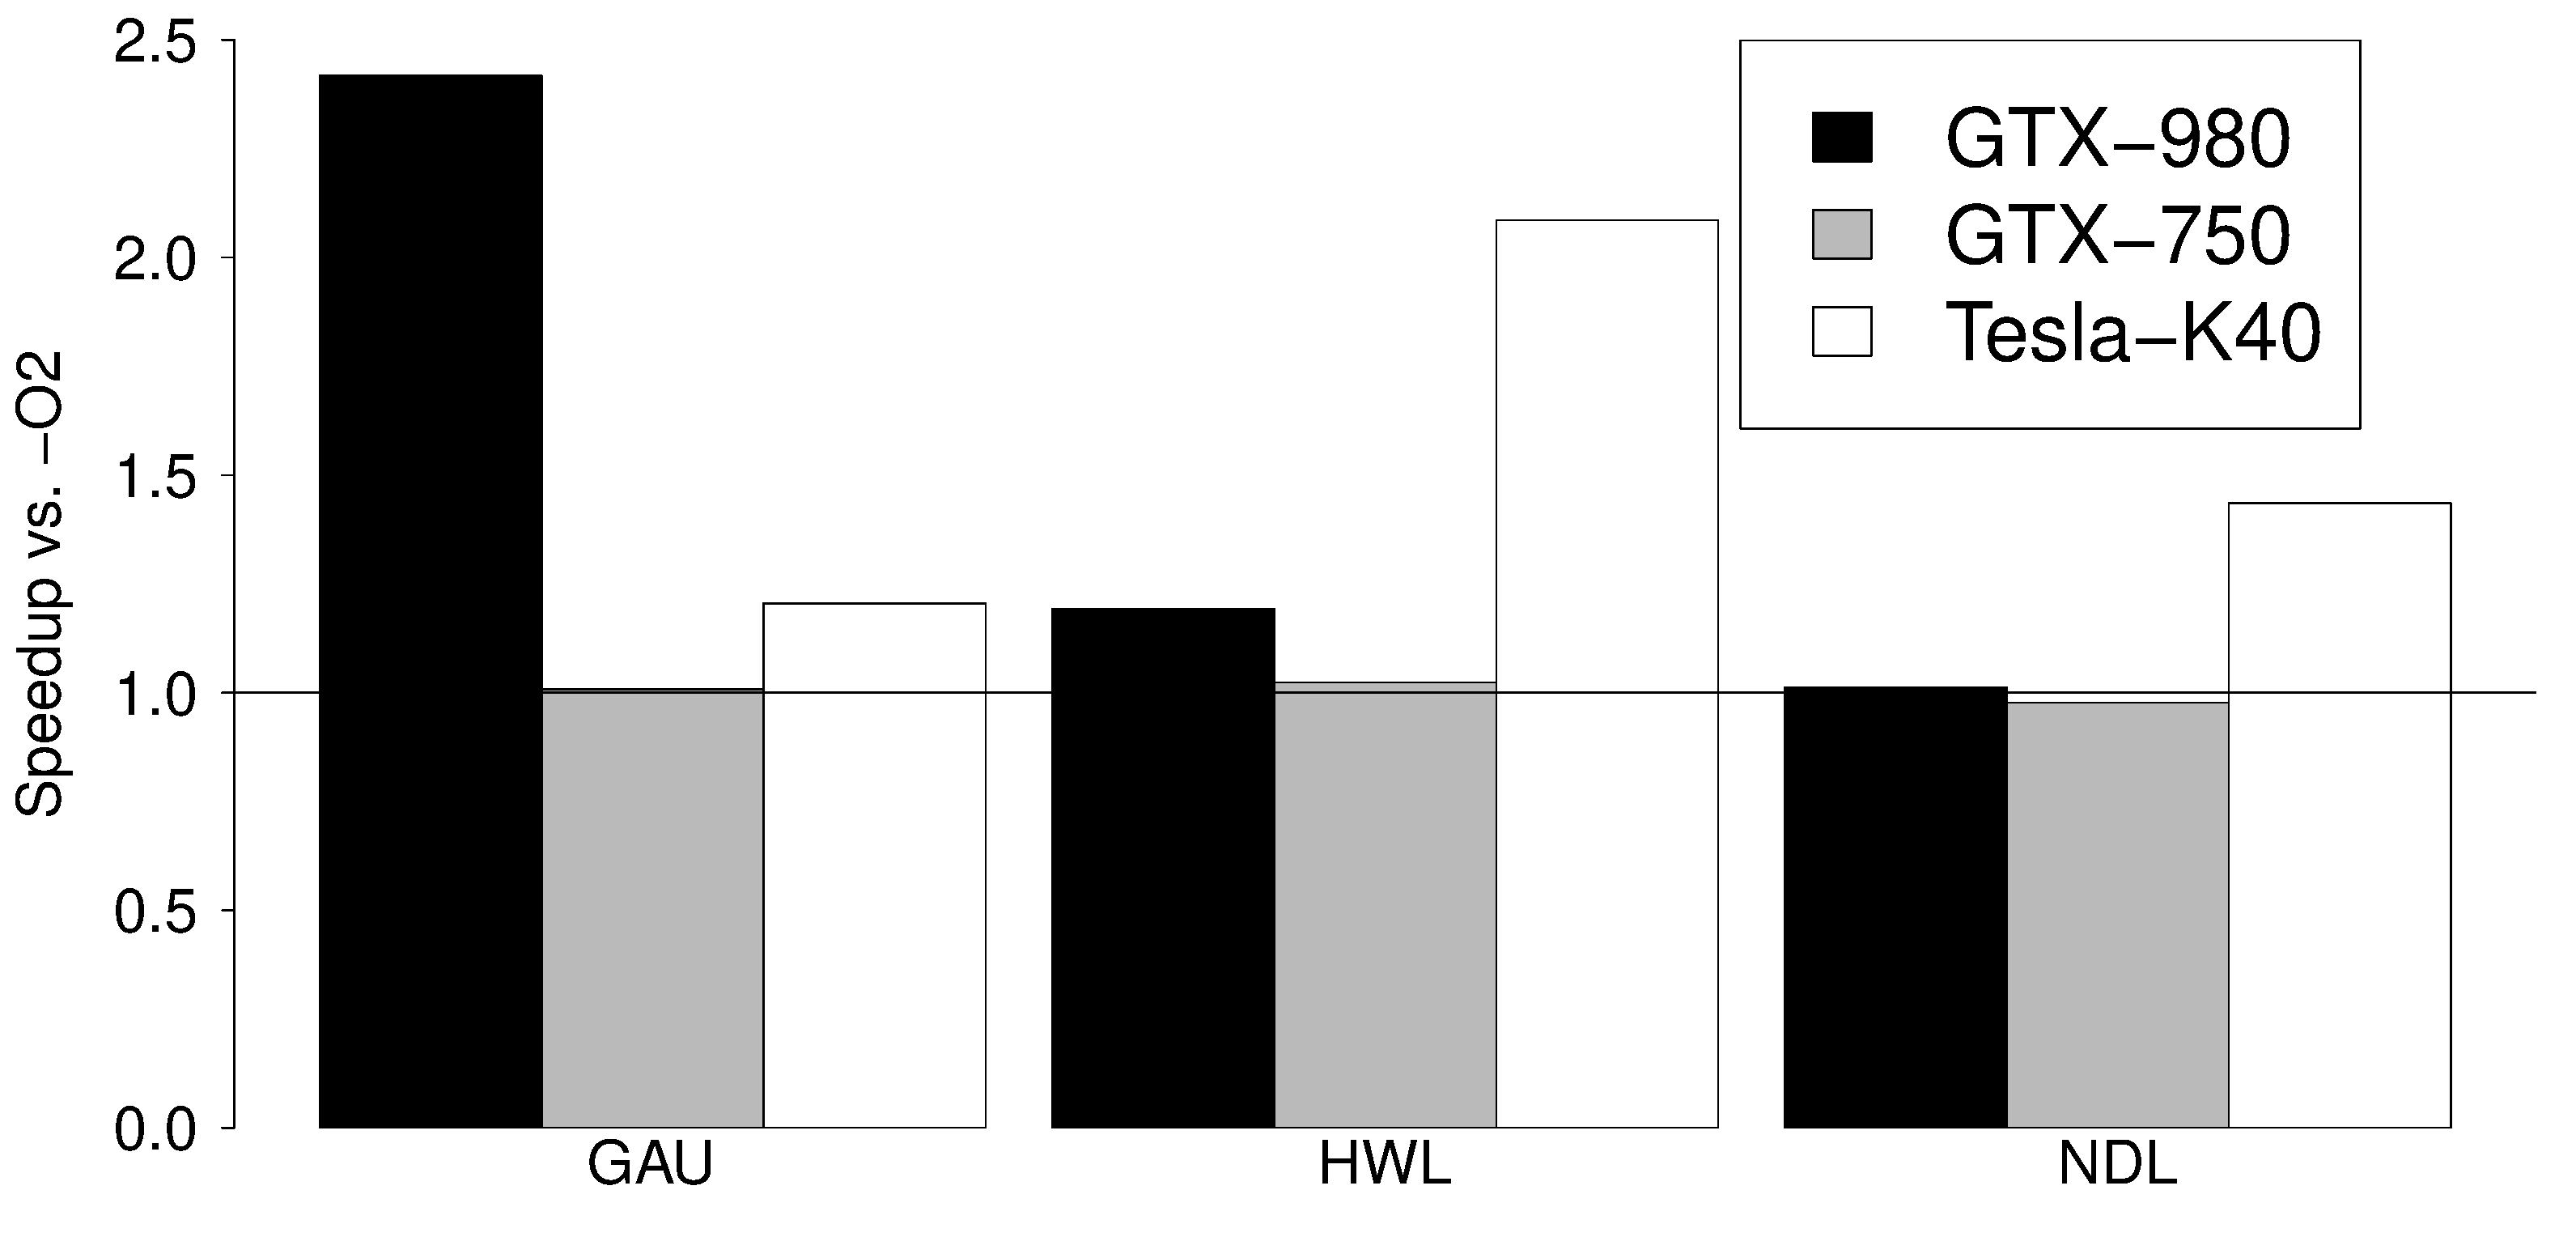
\includegraphics[scale=.15]{./images/RodiniaSummary.eps}
        \caption{Summary of the biggest speedups achieved versus \emph{-O2} in the Rodinia applications}
        \label{fig:rodiniasummary}
    \end{minipage}%
    \hfill
    \begin{minipage}{.48\textwidth}
        \centering
        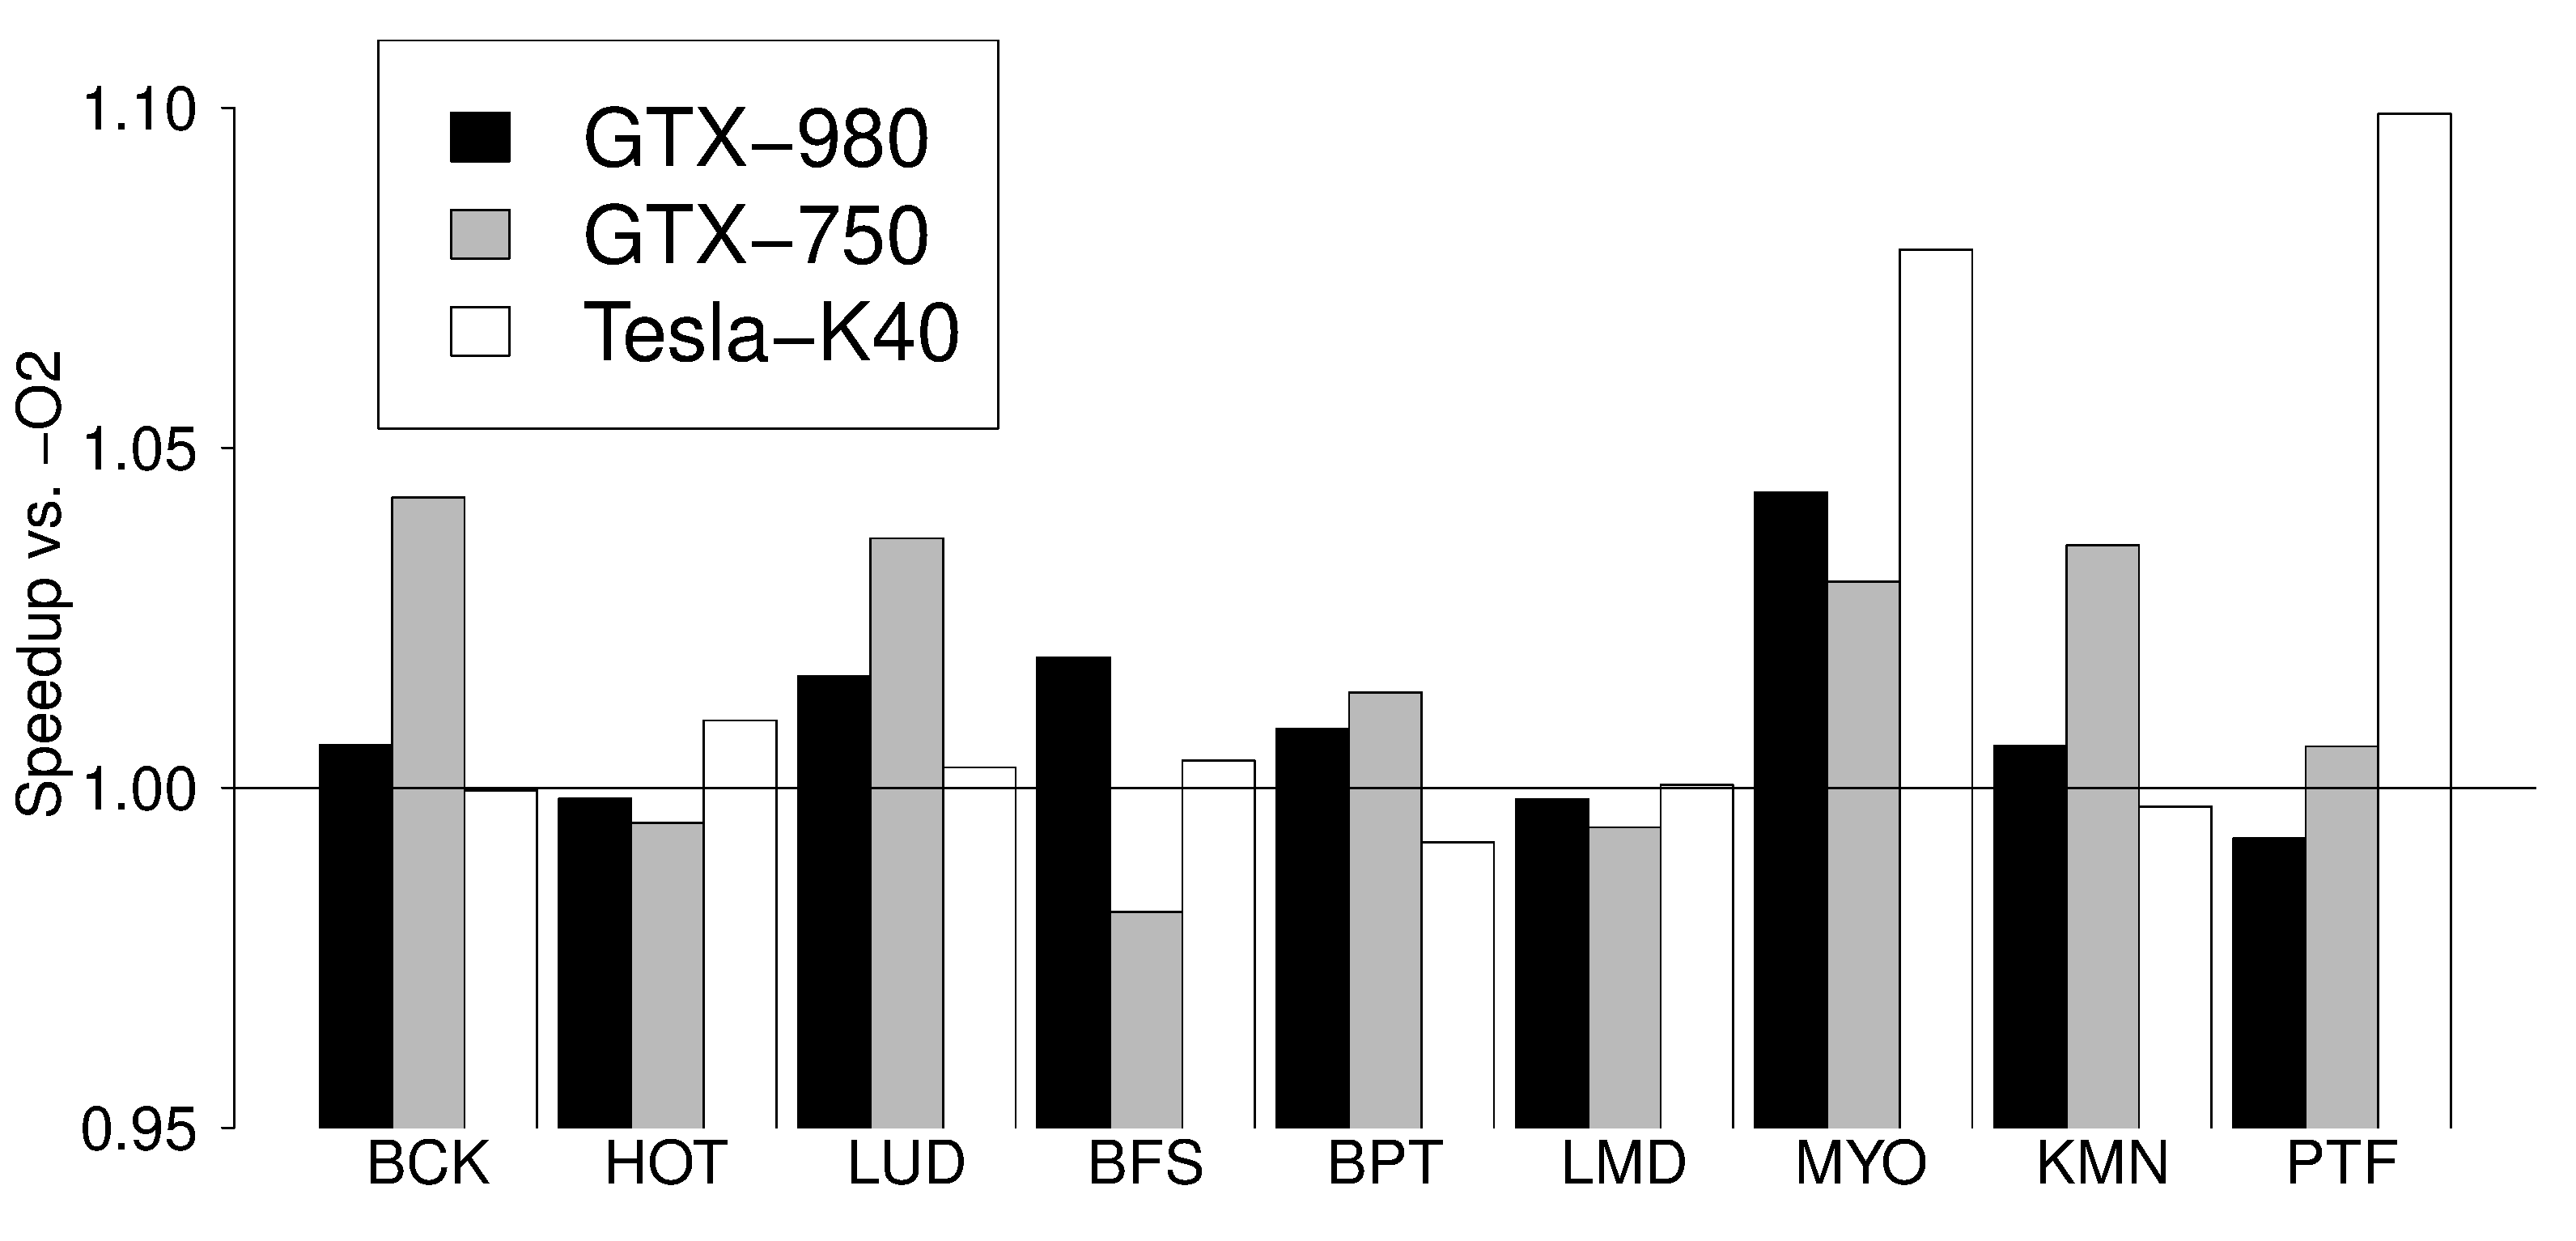
\includegraphics[scale=.15]{./images/RodiniaSummary_small.eps}
        \caption{Summary of the smaller speedups achieved versus \emph{-O2} in the Rodinia applications}
        \label{fig:rodiniasummarysmall}
    \end{minipage}%
\end{figure}

We do not know precisely which hardware characteristics impacted performance
the most.  Although more experiments are needed to confirm the following
hypothesis, we believe that the Maxwell GPUs, the GTX 980 and GTX 750, had
differing results from the Tesla K40 because they are consumer grade GPUs,
producing not so precise results and with different default optimizations. The
similarities between the compute capabilities of the GTX GPUs could also
explain the observed differences from the K40. Finally, the overall greater
computing power of the GTX 980 could explain its differing results from the GTX
750, since the GTX 980 has a greater number of Cores, SMs/Cores, Bandwidth,
Bus, Clock and Global Memory.

\subsubsection{Autotuner Performance}

This section presents an assessment of the autotuner's performance.
Figures~\ref{fig:K40hwBest}, \ref{fig:980gauBest}, \ref{fig:K40ptfBest} and
\ref{fig:K40myoBest} present the performance of the best solution found by the
autotuner versus the time these solutions were found, in seconds since the
beginning of the tuning process. The Figures show the evolution of the
autotuned solution for the best results in our experiments, the Heart Wall
problem (HWL) and the Gaussian Elimination problem (GAU) in the GTX 980, and
the Path Finder problem (PTF) and the Myocyte problem (MYO) in the Tesla K40.

The points in each graph represent the performance, in the y-axis, of the best
configuration found at the corresponding tuning time, shown in the x-axis. The
leftmost point in each graph represents the performance of a configuration
chosen at random by the autotuner. Each subsequent point represents the
performance of the best configuration found so far.

Note that the autotuner is able to quickly improve upon the initial random
configuration, but the rate of improvement decays over tuning time. The
duration of all tuning runs was two hours, or 7200 seconds.  The rightmost
point in each graph represents the performance of the last improving
configuration found by the autotuner. After the tuning time of this
configuration, the autotuner did not find any improving configuration until the
end of its tuning run.

The autotuner used the mean of 10 performance measurements of a given
configuration as the fitness value, reducing fluctuations and improving the
measurement's accuracy. This is reflected in the proximity of the measurements
reported by the autotuner during tuning, shown in figures~\ref{fig:K40hwBest},
\ref{fig:980gauBest}, \ref{fig:K40ptfBest} and \ref{fig:K40myoBest} and the
mean values of 10 measurements of the final solution, shown in the
corresponding figures~\ref{fig:K40hwl}, \ref{fig:980gau}, \ref{fig:K40ptf} and
\ref{fig:K40myo}.

\begin{figure}[htpb]
    \centering
    \begin{minipage}{.48\textwidth}
        \centering
        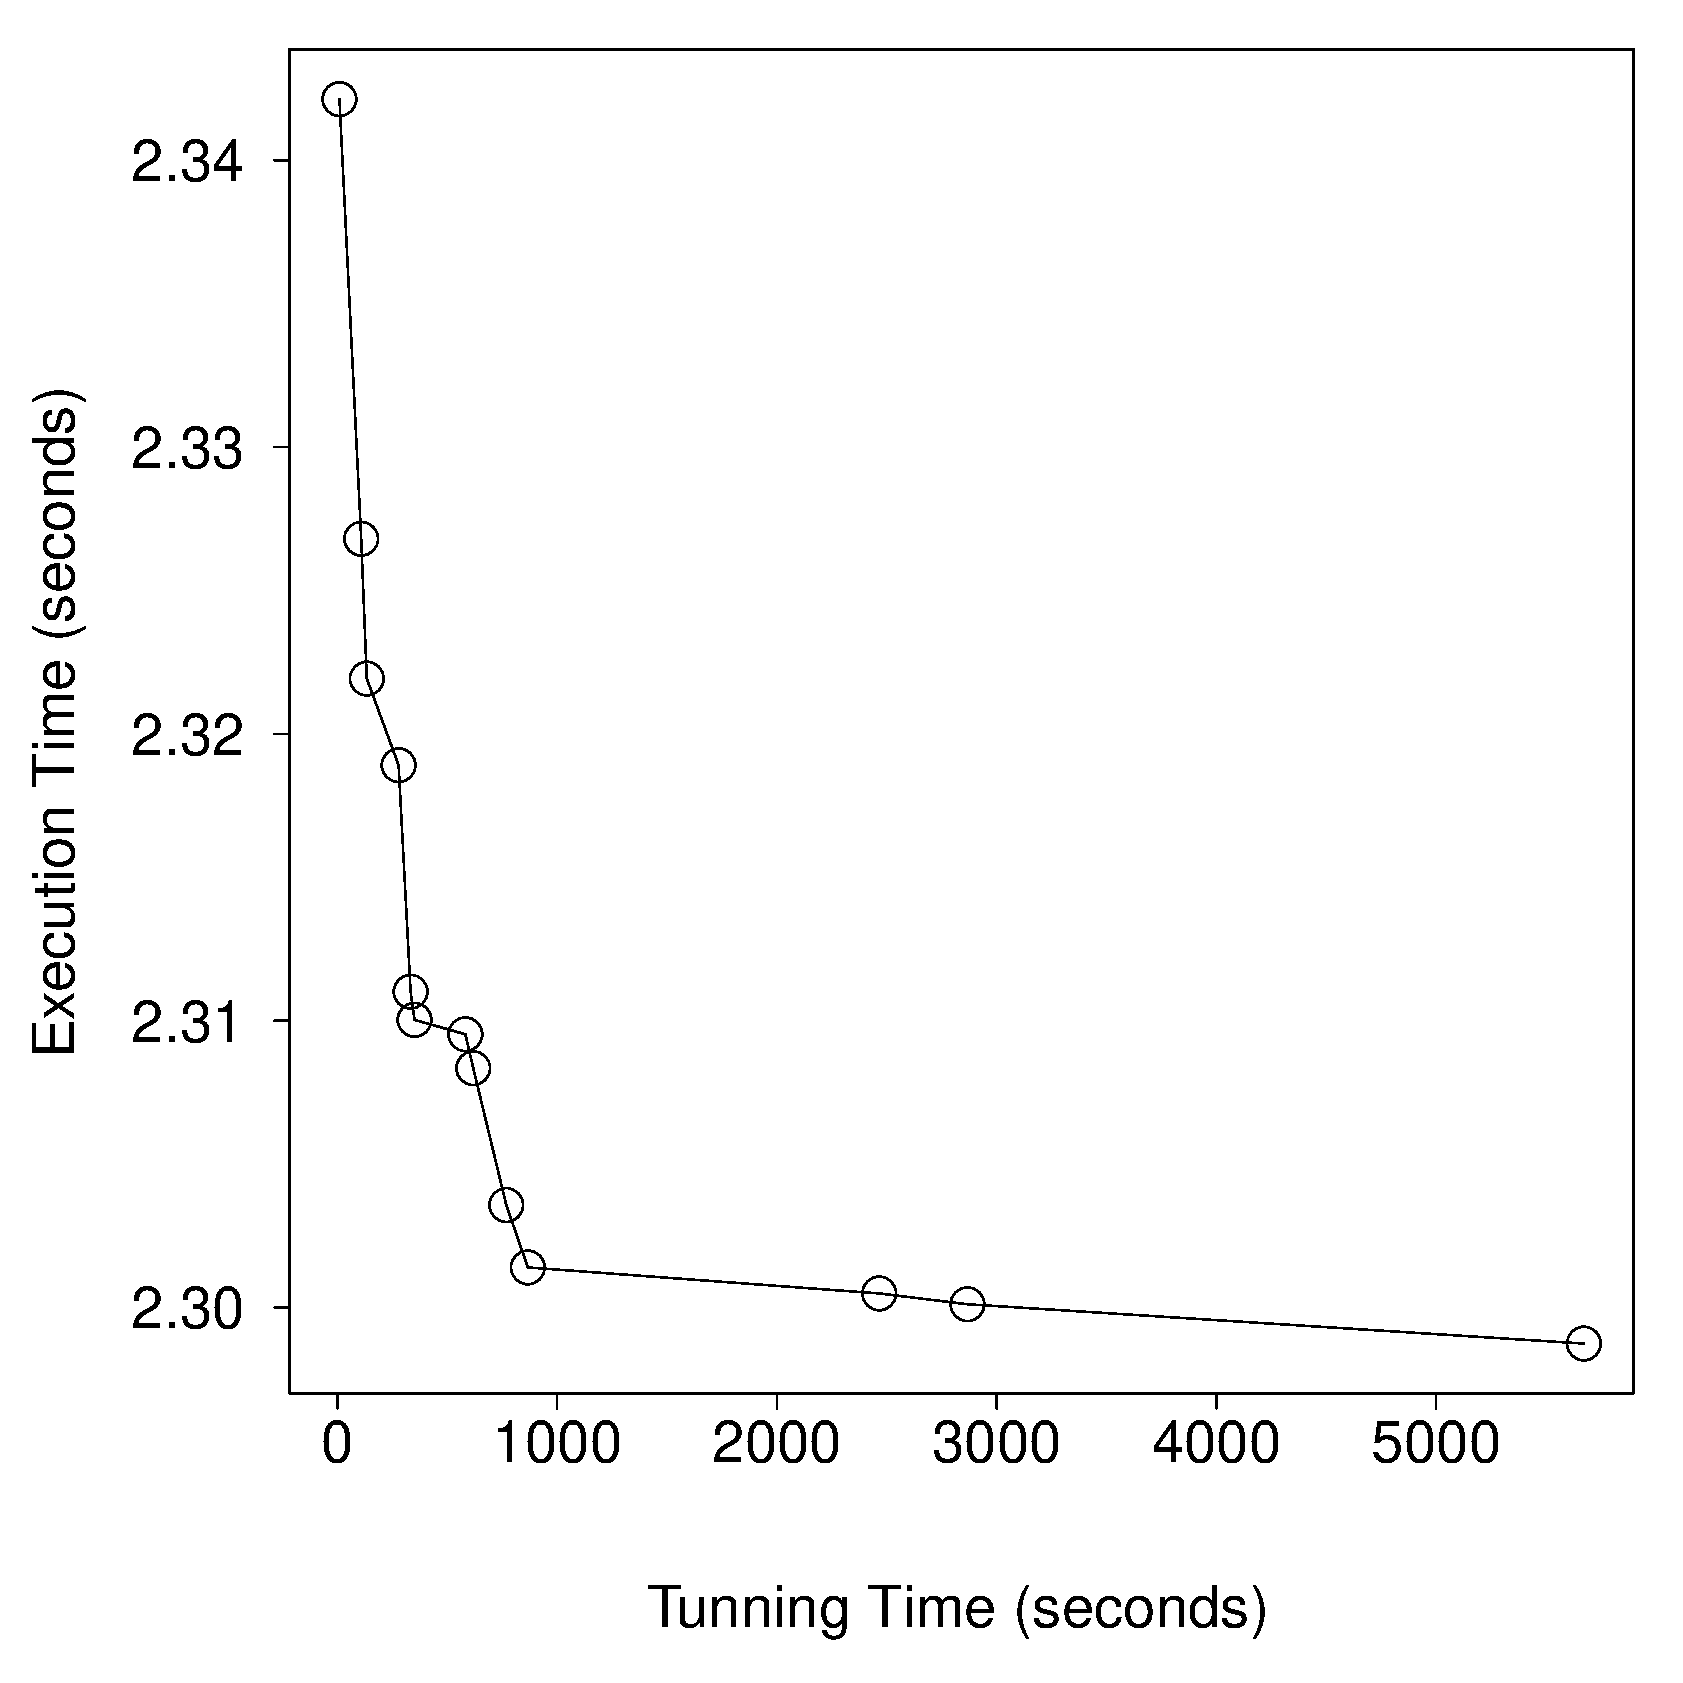
\includegraphics[scale=.22]{./images/heartwall-0-Tesla-K40-Best.eps}
        \caption{Best solutions found by the autotuner over time for the Heart Wall problem (HWL) in the Tesla K40}
        \label{fig:K40hwBest}
    \end{minipage}%
    \hfill
    \begin{minipage}{.48\textwidth}
        \centering
        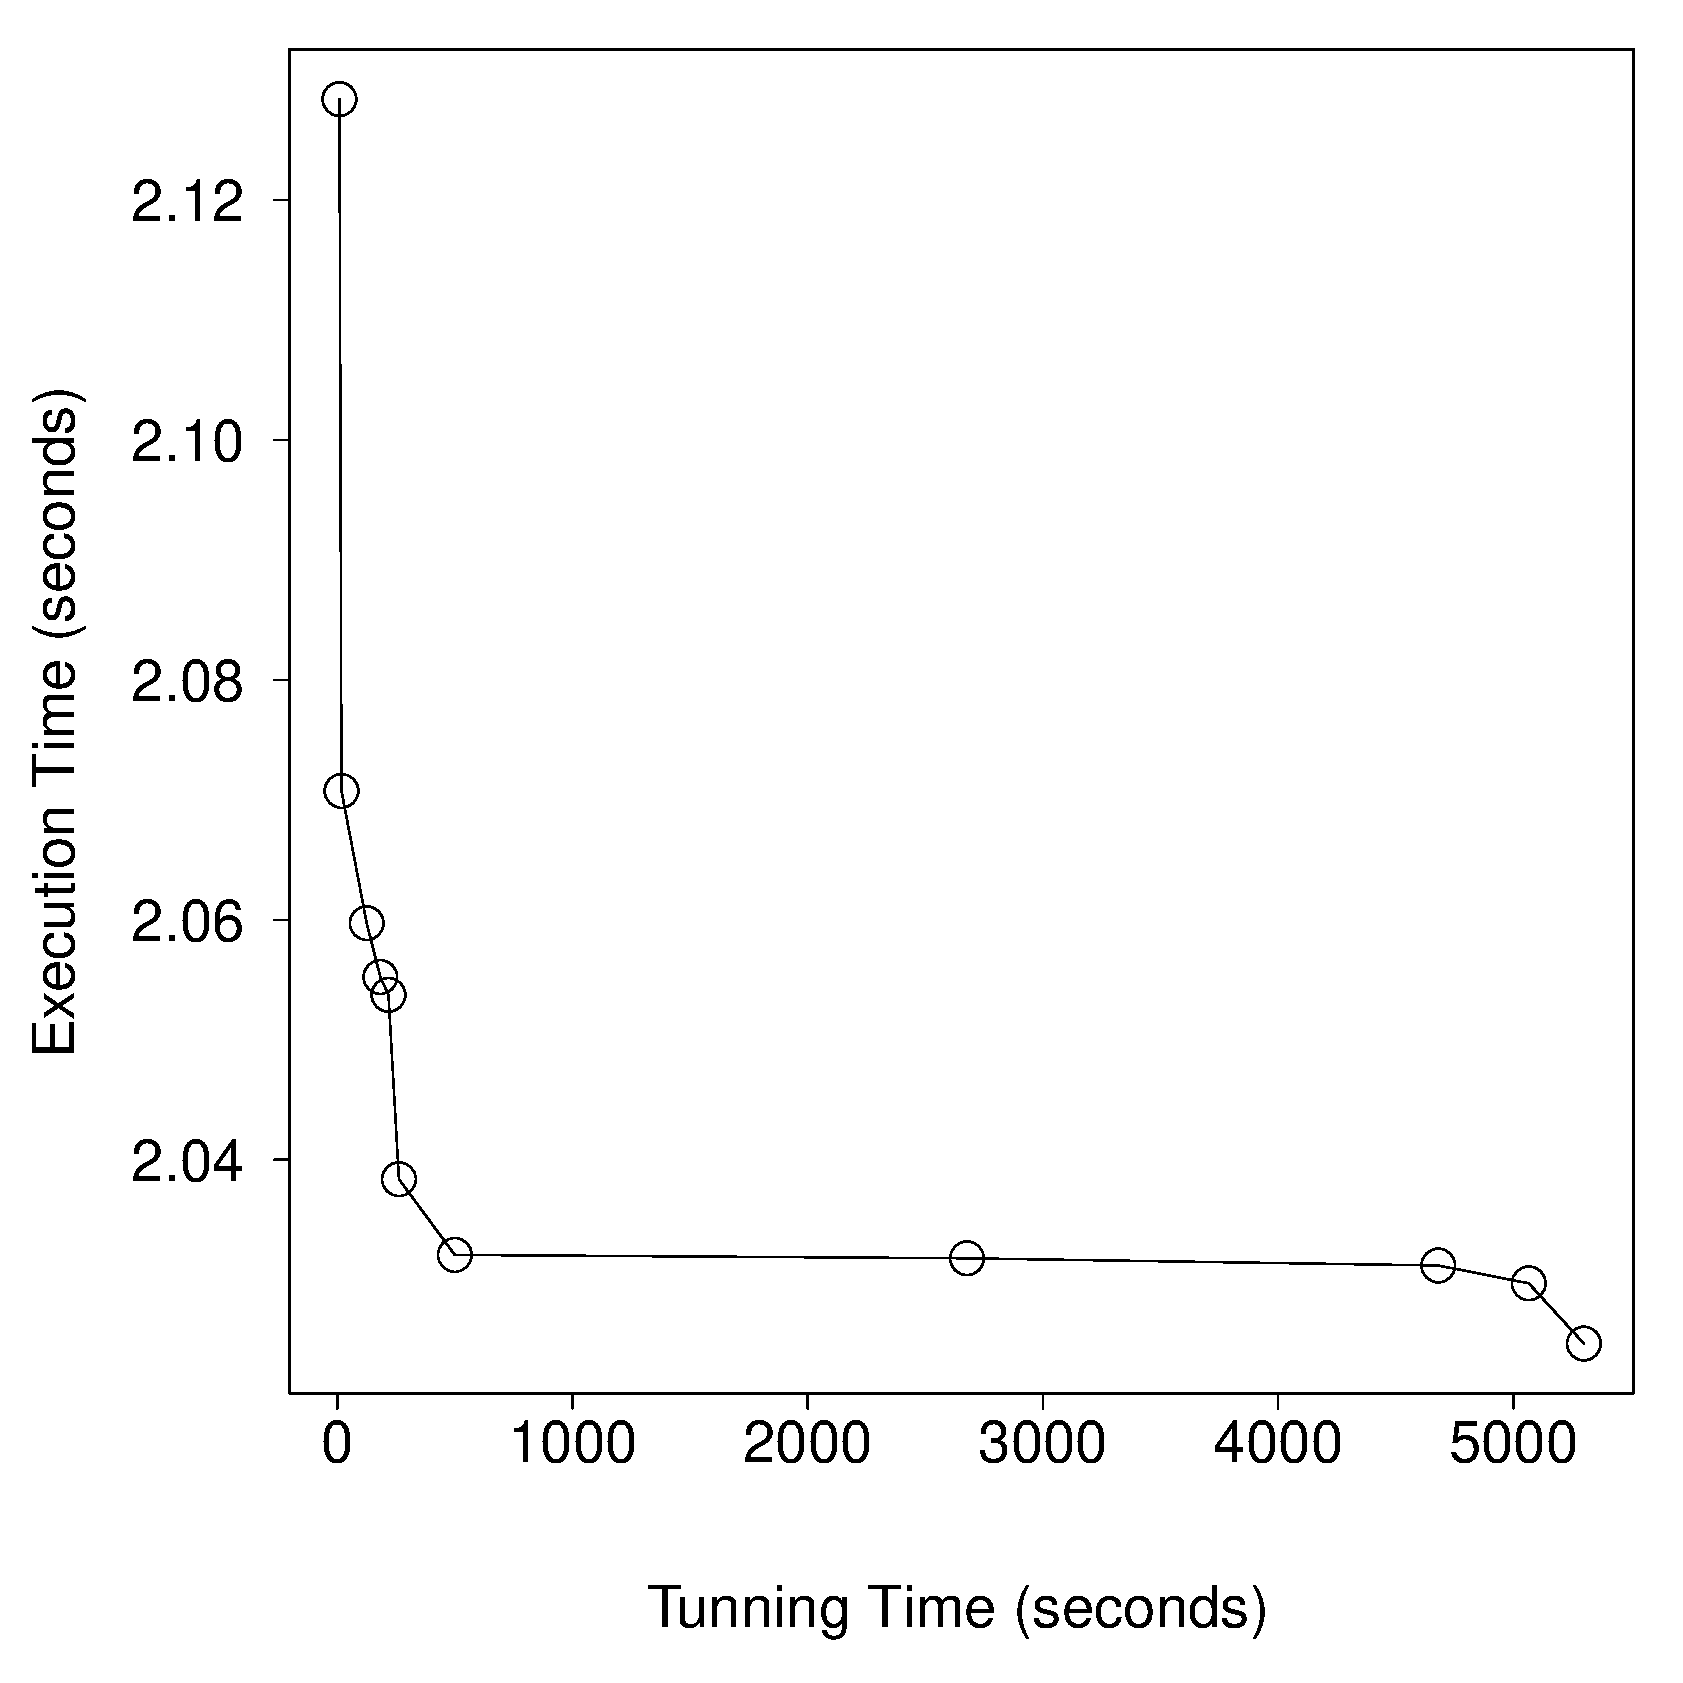
\includegraphics[scale=.22]{./images/gaussian-0-GTX-980-Best.eps}
        \caption{Best solutions found by the autotuner over time for the Gaussian Elimination problem (GAU) in the GTX 980}
        \label{fig:980gauBest}
    \end{minipage}%

    \begin{minipage}{.48\textwidth}
        \centering
        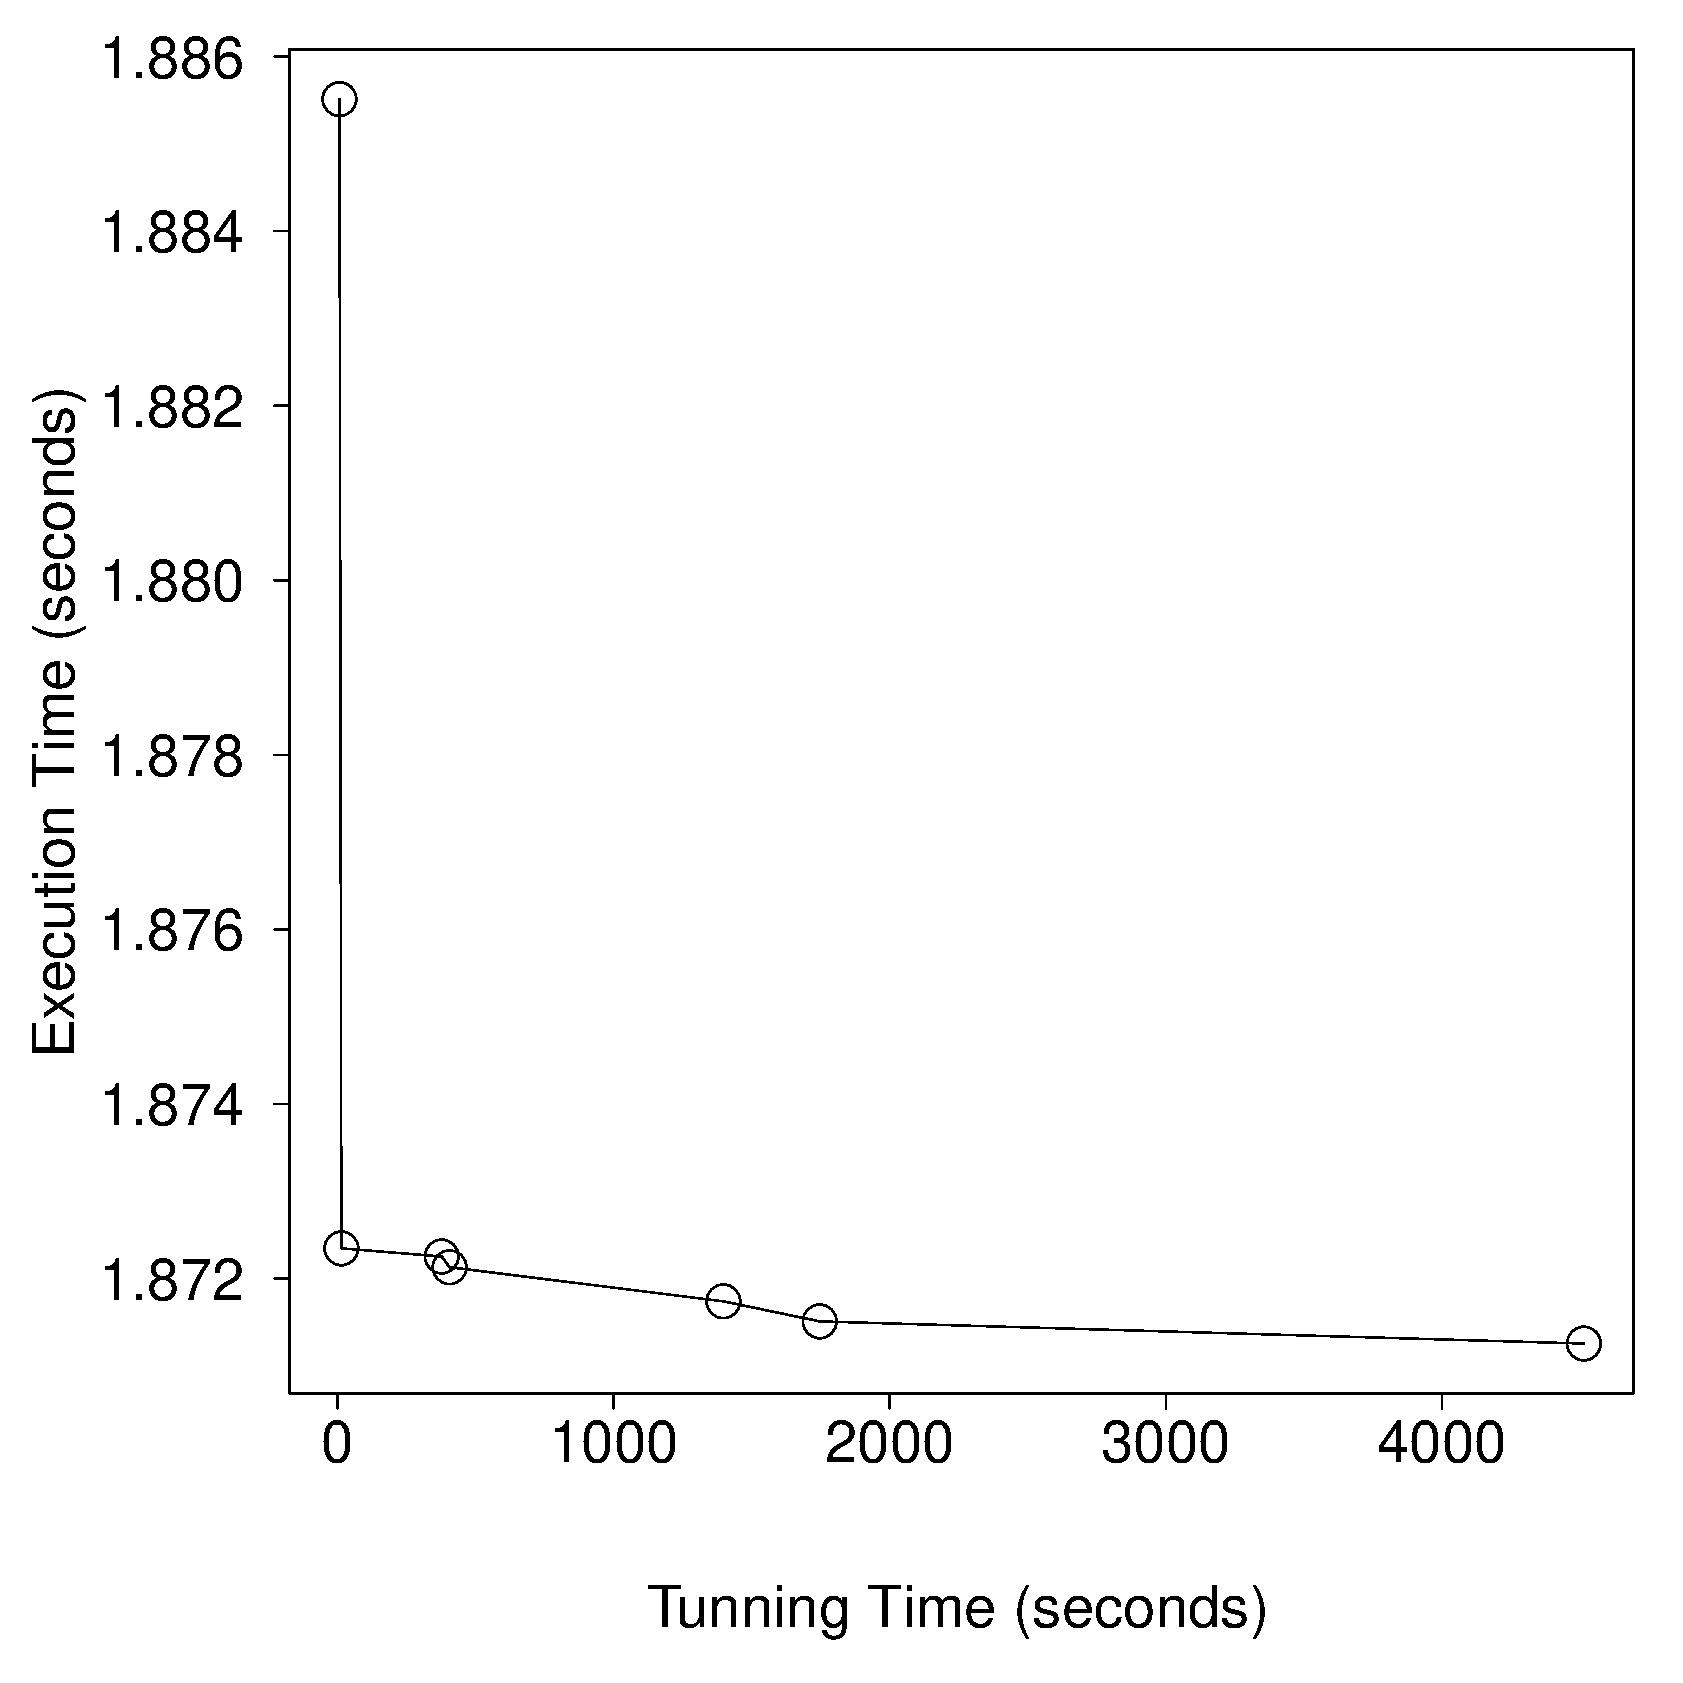
\includegraphics[scale=.22]{./images/Pathfinder-0-Tesla-K40-Best.eps}
        \caption{Best solutions found by the autotuner over time for the Path Finder problem (PTF) in the Tesla K40}
        \label{fig:K40ptfBest}
    \end{minipage}%
    \hfill
    \begin{minipage}{.48\textwidth}
        \centering
        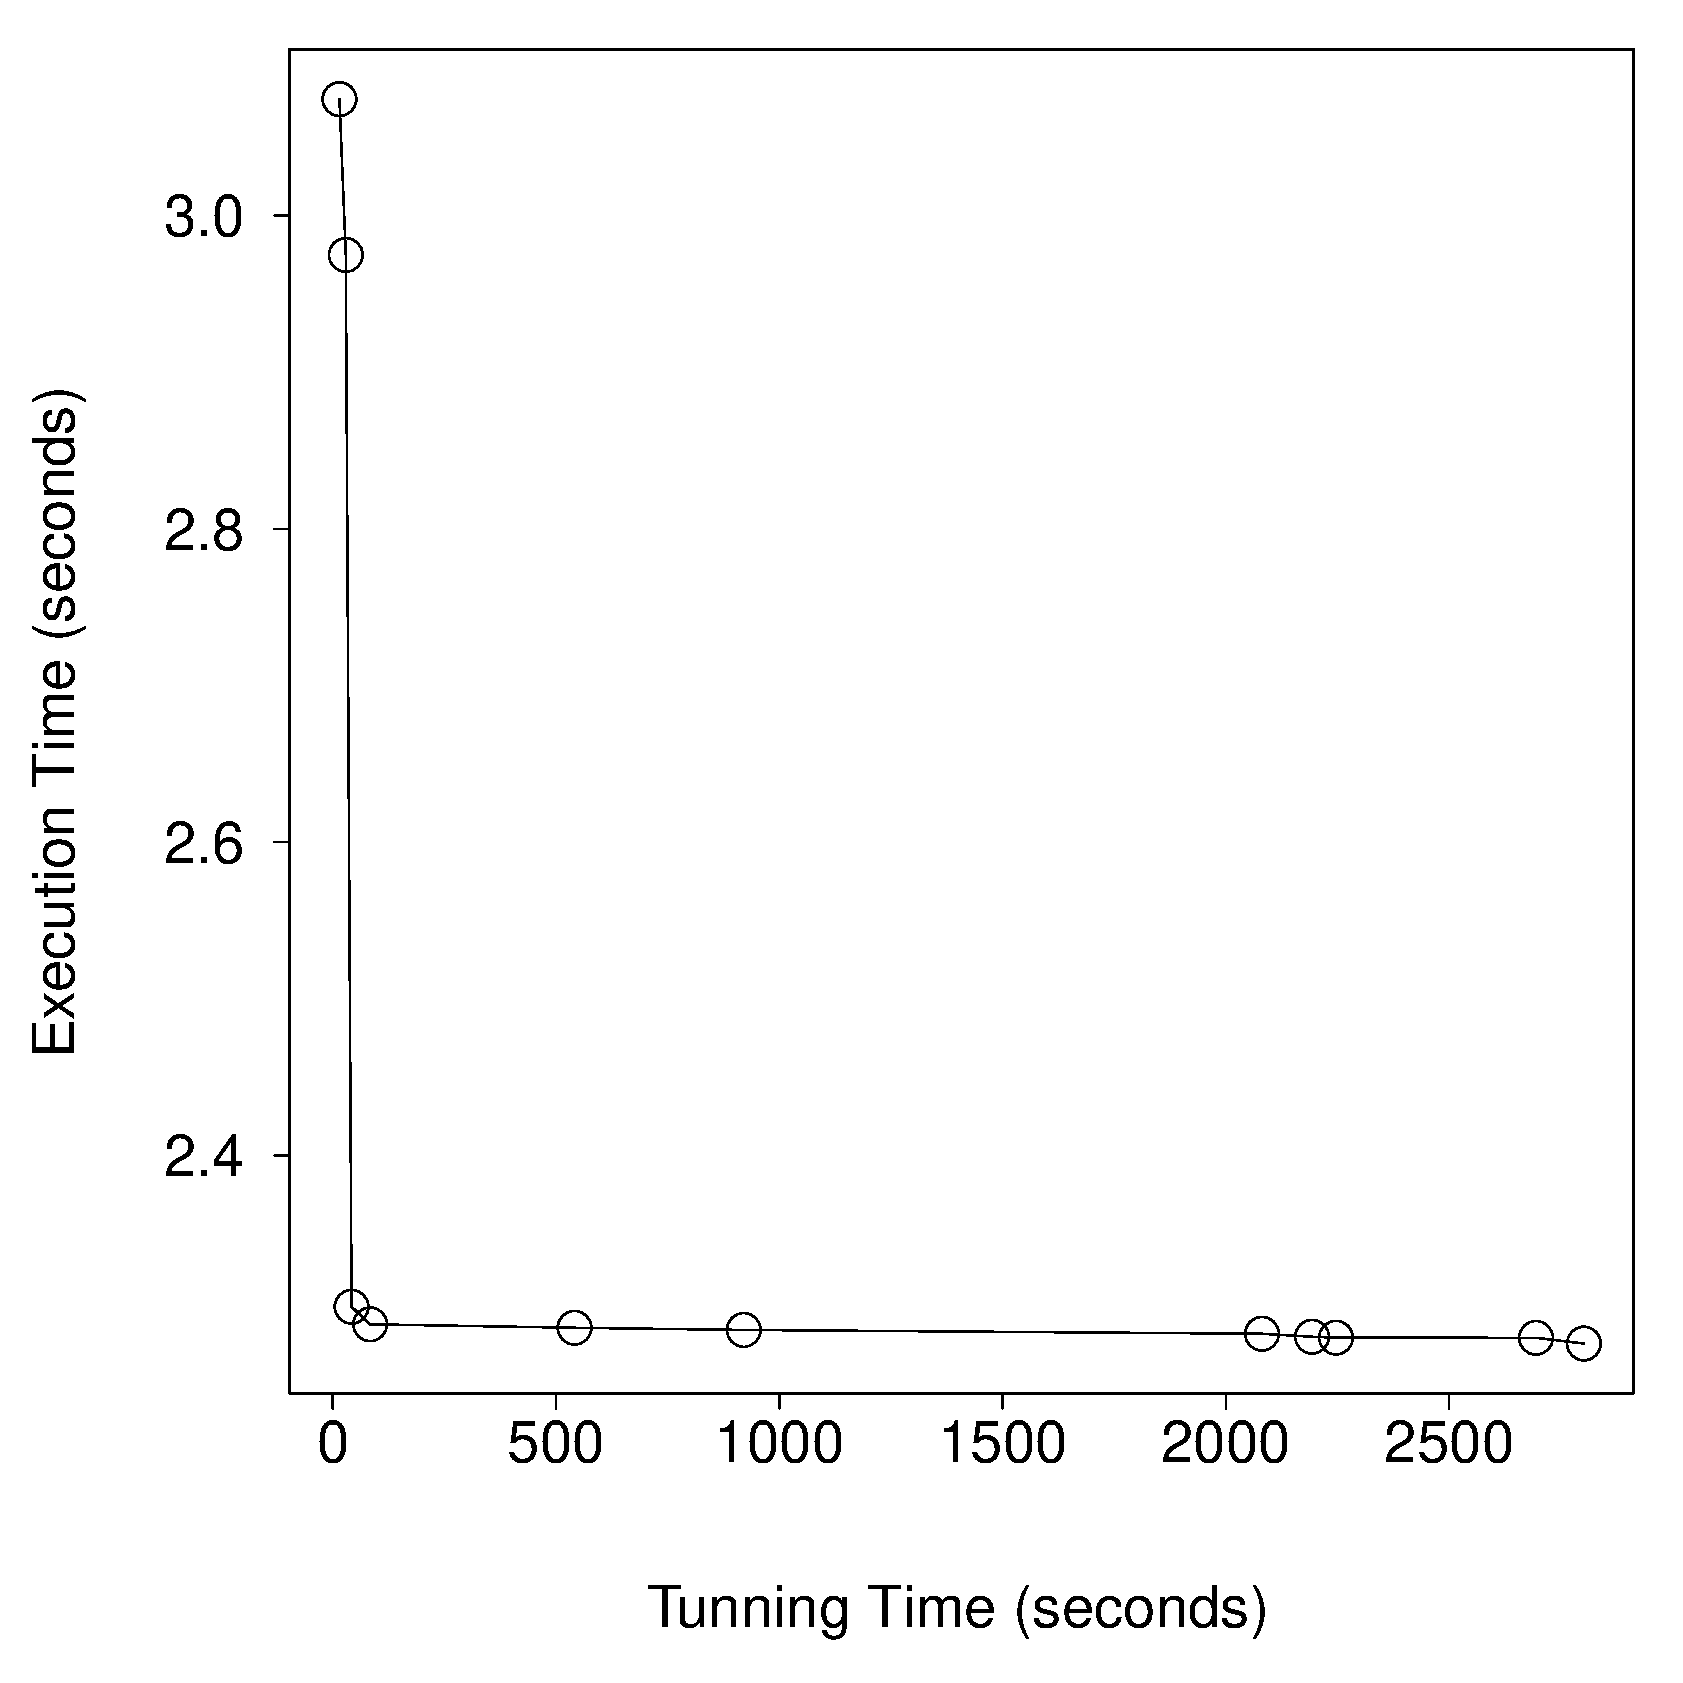
\includegraphics[scale=.22]{./images/myocyte-0-Tesla-K40-Best.eps}
        \caption{Best solutions found by the autotuner over time for the Myocyte problem (MYO) in the Tesla K40}
        \label{fig:K40myoBest}
    \end{minipage}
\end{figure}

\subsubsection{Parameter Selection}

\begin{table}[htpb]
    \centering
    \footnotesize
    \begin{tabular}{ccc}
        \toprule
        \textbf{Flag} & \textbf{Cluster 0 (17\%)} & \textbf{Cluster 1 (83\%)} \\\midrule
        no-align-double               & on     & on     \\\midrule
        use\_fast\_math               & on     & on     \\\midrule
        preserve-relocs               & off    & off    \\\midrule
        relocatable-device-code       & true   & false  \\\midrule
        ftz                           & true   & true   \\\midrule
        prec-div                      & true   & false  \\\midrule
        prec-sqrt                     & true   & true   \\\midrule
        fmad                          & false  & false  \\\midrule
        allow-expensive-optimizations & false  & true   \\\midrule
        gpu-architecture              & sm\_20 & sm\_50 \\\midrule
        def-load-cache                & cv     & ca     \\\midrule
        opt-level                     & 1      & 3      \\\midrule
        maxrregcount                  & 42     & 44.6   \\\bottomrule
        \end{tabular}
    \caption{Parameter clusters for all Rodinia problems in the GTX 750}
    \label{tab:750RodiniaClusters}
\end{table}

We attempted to associate compilation parameters to applications and GPUs using
WEKA's~\cite{holmes1994weka} clustering algorithms. Although we could not find
significant relations for most applications we detected that the
\texttt{ftz=true} in MMS and the Compute Capabilities 3.0, 5.0 and 5.2 in GAU
caused the speedups observed in the GTX 980 for these applications.
Table~\ref{tab:750RodiniaClusters} shows clusters obtained with the K-means
WEKA algorithm for autotuned parameter sets for the Rodinia Benchmark in the
GTX 750. Unlike most clusters found for all GPUs and problems, these clusters
did not contain an equal number of instances. The difficulty of finding
associations between compiler optimizations, applications and GPUs justifies
the autotuning of compiler parameters in the general case.

\subsection{Summary}
\label{subsec:GPUconcl}

This study showed that it is possible to improve the performance of GPU
applications applying empirical and automatic tuning techniques. Our results
and clustering attempts emphasize the importance of automatic optimization
techniques by showing that different compilation options have to be selected in
order to achieve performance improvements in different GPUs and that it is
difficult to associate compiler optimization parameters, applications and GPUs.

An interesting direction for future studies is including application parameters
and options for the GCC compiler, which also composes the CUDA compilation
chain. Section~\ref{} will discuss our efforts on spreading the autotuning
of CUDA compiler parameters to the NVIDIA CUDA programmer community.

\todo[inline,author=Pedro,color=cyan]{Fix this reference}

\section{Selecting Parameters for High-Level Synthesis for FPGAs}
\label{sec:FPGA}

FPGAs are reprogrammable circuits that enable writing specialized hardware
specifications for a variety of applications using the same chip.
High-Performance Computing tasks that require low power and latency
increasingly switch to FPGAs from GPUs. Hardware specifications are written
using low-level languages such as Verilog and VHDL, making a challenge for
software engineers to leverage FPGA capabilities.  This became increasingly
relevant by the adaptation of FPGAs for data
centers~\cite{caulfield2016cloud}\footnote{\url{https://cloud.baidu.com/product/fpga.html}
[Accessed in 28/07/2017], \\ and
\url{https://aws.amazon.com/ec2/instance-types/f1/} [Accessed in 28/07/2017]},
a field dominated by software engineers.

Essential support for software engineers can be provided by High-Level
Synthesis (HLS), the process of generating hardware descriptions from
high-level code.  HLS lowers the complexity of hardware design from the point
of view of software engineering and has become increasingly viable as part of
the FPGA design methodology, with support from vendor HLS
tools~\cite{singh2011implementing, feist2012vivado} for C/C++ and OpenCL. The
benefits of higher-level abstractions come with the cost of decreased
application performance, making FPGAs less viable as accelerators.  Thus,
optimizing HLS still requires domain expertise and exhaustive or manual
exploration of design spaces and configurations.

High-Level Synthesis is an \NP{}-Complete problem~\cite{canis2015legup} and a
common strategy for its solution involves the divide-and-conquer
approach~\cite{coussy2009introduction}.  The most important sub-problems to
solve are \textit{scheduling}, where operations are assigned to specific clock
cycles, and \textit{binding}, where operations are assigned to specific
hardware functional units, which can be shared between operations.
LegUp~\cite{canis2013legup} is an open-source HLS tool implemented as a
compiler pass for the LLVM Compiler Infrastructure~\cite{chris2004llvm}.  It
receives code in LLVM's intermediate representation as input and produces as
output a hardware description in Verilog.  LegUp exposes configuration
parameters of its HLS process, set with a configuration file.

This section presents an autotuner for LegUp HLS parameters implemented using
the OpenTuner framework.  The autotuner targeted 8 hardware metrics obtained
from
Quartus~\footnote{\url{https://www.altera.com/products/design-software/fpga-design/quartus-prime/overview.html}
[Accessed in 18/07/2017]}, for applications of the CHStone HLS benchmark
suite~\cite{hara2008chstone} in the Intel StratixV FPGA.  The program to be
configured here is LegUp and the search space is composed of approximately
$10^{126}$ possible combinations of HLS parameters.  Such a large search space
is unfeasible to search exhaustively or by hand.

One of the obstacles we faced was making accurate predictions for hardware
metrics from a set of HLS parameters. We decided to run our autotuner with the
metrics reported by the lengthier process of hardware synthesis instead.  Our
autotuner's virtualized implementation enables deployment in distributed
environments.  We present data showing that our autotuner found optimized HLS
parameters for CHStone applications that decreased the \textit{Weighted
Normalized Sum} (\textbf{WNS}) of hardware metrics by up to $21.5\%$ on
average, and $10\%$ on average.

\subsection{Large Measurement Time}
\label{sec:bigtime}

The defining characteristic of this autotuning experiment is the potentially
large time it takes to synthesize hardware from specifications in hardware
description languages, which takes from minutes to hours. The process of
generating those specifications from high-level C code is much faster in
comparison, taking only seconds. In contrast to the previous section, the
applications used in this autotuning experiment had a \textit{large measurement
time}. Section~\ref{sec:FPGAautotuner} describes in more detail the High-Level
Synthesis process.

\begin{figure}[htpb]
    \centering
    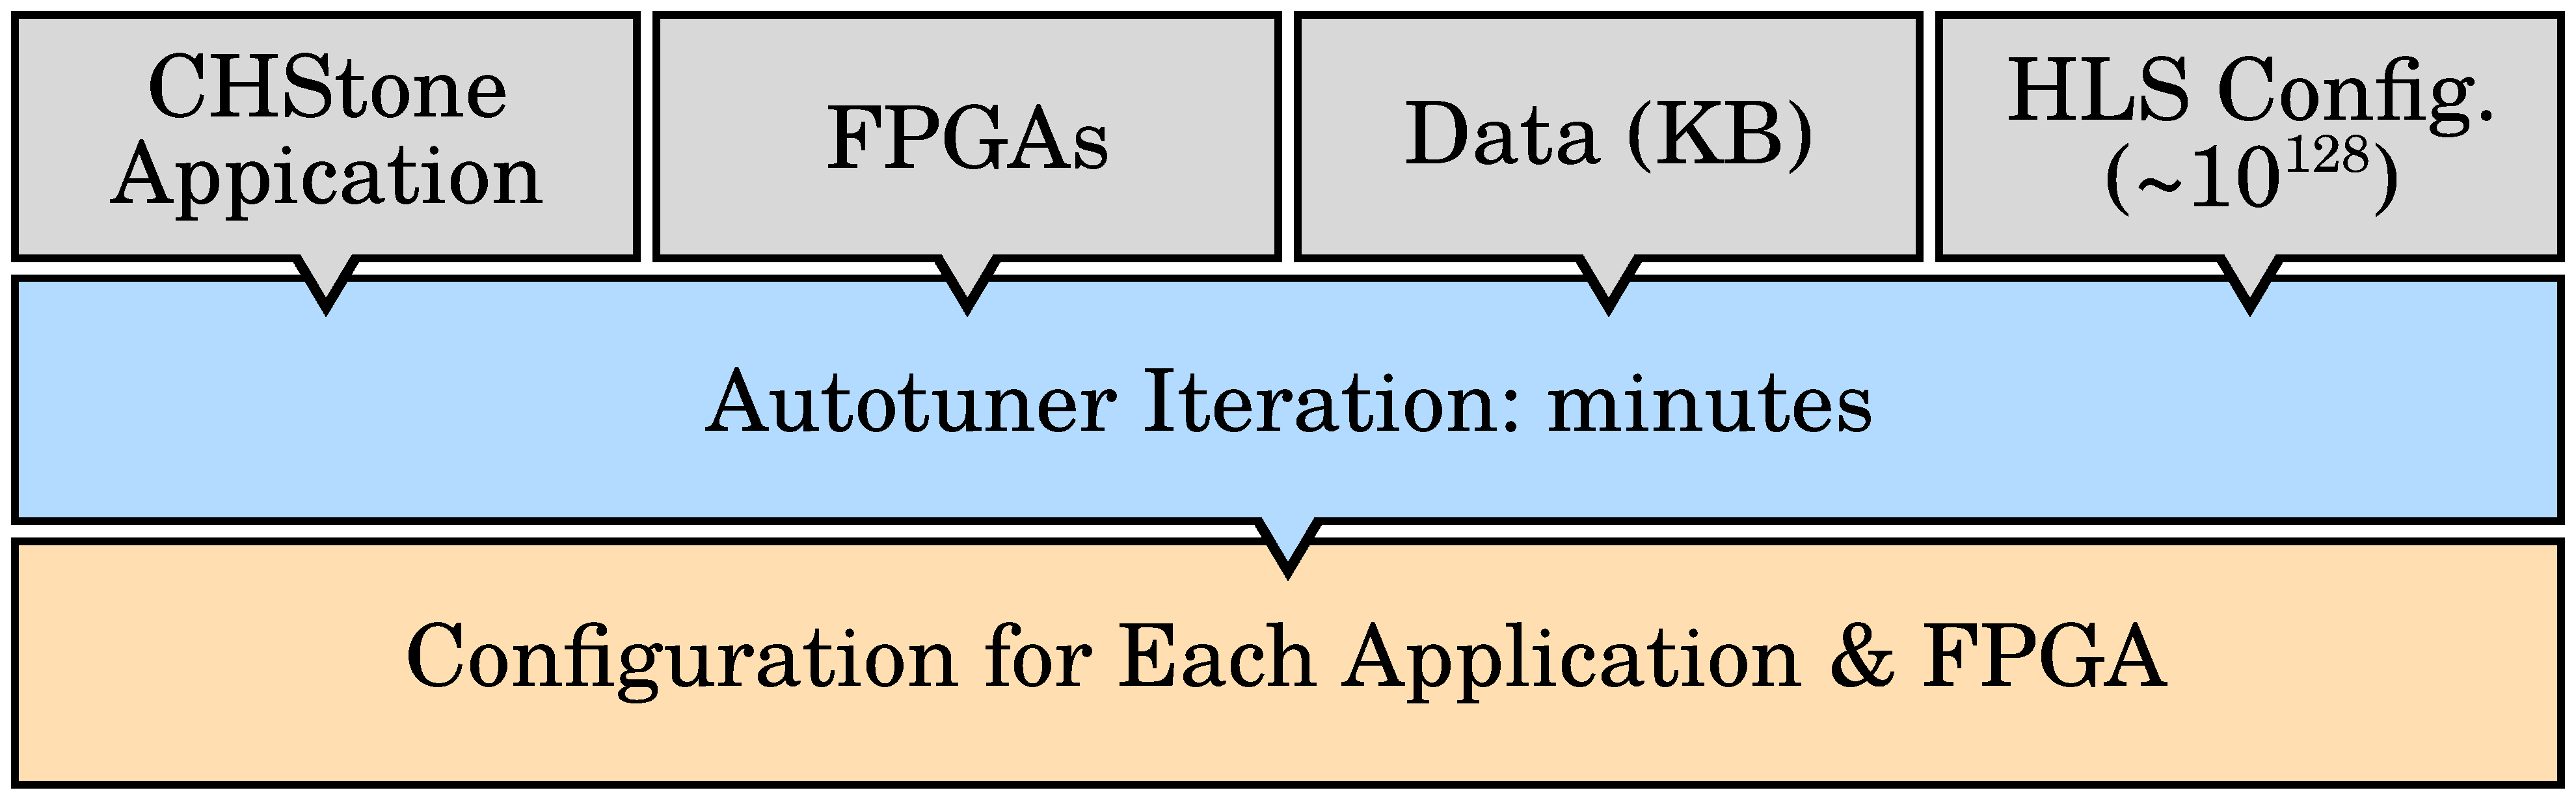
\includegraphics[width=.65\textwidth]{./images/overview_fpgas_small}
    \caption{Autotuner representation and time scale of our experiments}
    \label{fig:overview-fpgas-small}
\end{figure}

Figure~\ref{fig:overview-fpgas-small} shows a representation of our autotuner
for this experiment, and illustrates its time scale.  The autotuner,
represented by the light blue box, receives as input a CHStone application, a
target FPGA, input data for the application in the order of Kilobytes and a
search space composed of LegUp's HLS parameters. The autotuner outputs an HLS
configuration for each application and FPGA.

\begin{figure}[htpb]
    \centering
    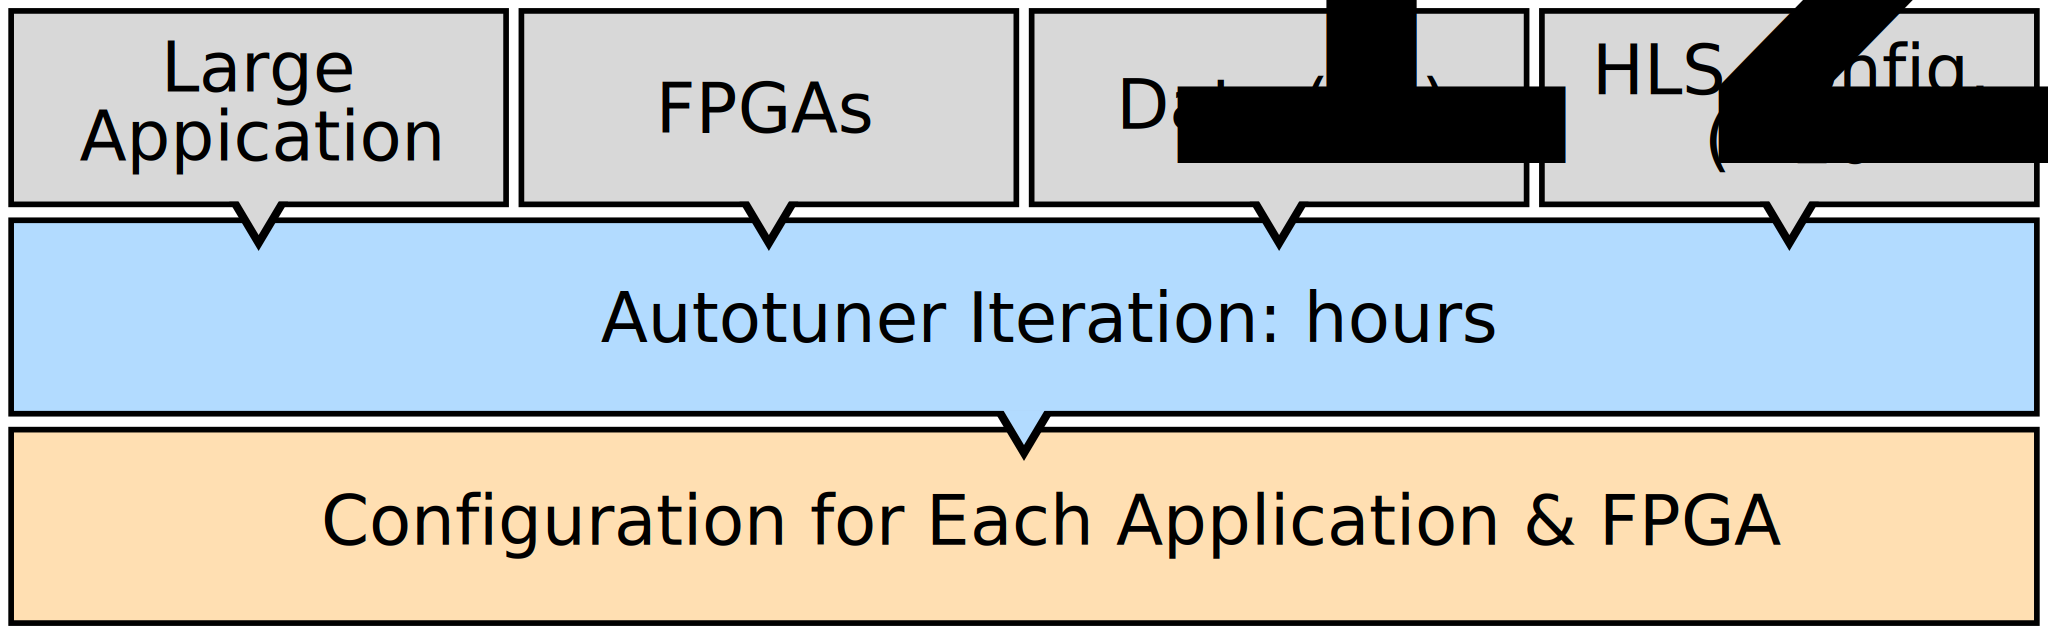
\includegraphics[width=.65\textwidth]{./images/overview_fpgas_big}
    \caption{Autotuner representation and time scale of more complex FPGA
    applications}
    \label{fig:overview-fpgas-big}
\end{figure}

The applications from CHStone, presented further in Table~\ref{tab:chstone},
are very simple benchmark applications, and generating hardware for them takes
time in the order of minutes. Generating hardware for more complex FPGA
applications can take several hours. Figure~\ref{fig:overview-fpgas-big} shows
a representation and time scale for an autotuner that targets complex FPGA
applications. Each iteration now takes several hours, and limits the
configurations that can be tested per hour.

We worked around this limitation in this experiment by implementing a
virtualized autotuner using Docker containers, which enabled parallel
measurements of different configurations. The lack of support in OpenTuner for
a distributed execution of measurements also limited this experiment, since our
already virtualized approach could explore more search space in the same time
if it was deployed in more connected machines.

Applications with large measurement time still present a challenge for our
current autotuning approach, even with a tool that can achieve distributed
execution of measurements, because the quality of the solutions still depend on
the velocity of exploration of the search space.  To mitigate this problem and
enable the autotuning of applications with large measurement times, which can
be thought of as\textit{expensive-to-evaluate functions}, we are going to study
the development of suitable experimental designs. We will work in this
direction in collaboration and supervision of professors Arnaud Legrand, Brice
Videau and Jean-Marc Vincent from the University of Grenoble Alpes.

\subsection{Background}
\label{sec:FPGAbackground}

In this section we discuss background work related to HLS tools,
and autotuning for FPGAs.

\paragraph{Tools for HLS}

Research tools for High-Level Synthesis have been developed as well as vendor
tools \cite{singh2011implementing, feist2012vivado}. Villareal \emph{et
al.}~\cite{villarreal2010designing} implemented extensions to the Riverside
Optimizing Compiler for Configurable Circuits (ROCCC), which also uses the LLVM
compiler infrastructure, to add support for generating VHDL from C code.
Implemented within GCC, GAUT~\cite{coussy2010gaut} is an open-source HLS tool
for generating VHDL from C/C++ code. Other HLS tools such as
Mitrion~\cite{kindratenko2007mitrion}, Impulse~\cite{antola2007novel} and
Handel~\cite{loo2002handel} also generate hardware descriptions from C code.
We refer the reader to the survey from Nane \emph{et al.}~\cite{nane2016survey}
for a comprehensive analysis of recent approaches to HLS.

\paragraph{Autotuning for FPGAs}

Recent works study autotuning approaches for FPGA compilation.  Xu et
al.~\cite{xu2017parallel} used distributed OpenTuner instances to optimize the
compilation flow from hardware description to bitstream.  They optimize
configuration parameters from the Verilog-to-Routing (VTR)
toolflow~\cite{luu2014vtr} and target frequency, wall-clock time and logic
utilization.  Huang et al.~\cite{huang2015effect} study the effect of LLVM pass
ordering and application in LegUp's HLS process, demonstrating the complexity
of the search space and the difficulty of its exhaustive exploration.  They
exhaustively explore a subset of LLVM passes and target logic utilization,
execution cycles, frequency, and wall-clock time.  Mametjanov \emph{et
al.}~\cite{mametjanov2015autotuning} propose a machine-learning-based approach
to tune design parameters for performance and power consumption.  Nabi and
Vanderbauwhede~\cite{nabi2016fast} present a model for performance and resource
utilization for designs based on an intermediate representation.

\subsection{Autotuner \& Search Space}
\label{sec:FPGAautotuner}

This section describes our autotuner implementation, the LegUp HLS parameters
selected for tuning, and the autotuning metrics used to measure the quality of
HLS configurations.

\subsubsection{Autotuner}

We implemented our autotuner with OpenTuner~\cite{ansel2014opentuner}, using
ensembles of search techniques to find an optimized selection of
LegUp~\cite{canis2015legup} HLS parameters, according to our cost function, for
11 of the CHStone~\cite{hara2008chstone} applications.

\begin{figure}[htpb]
    \centering
    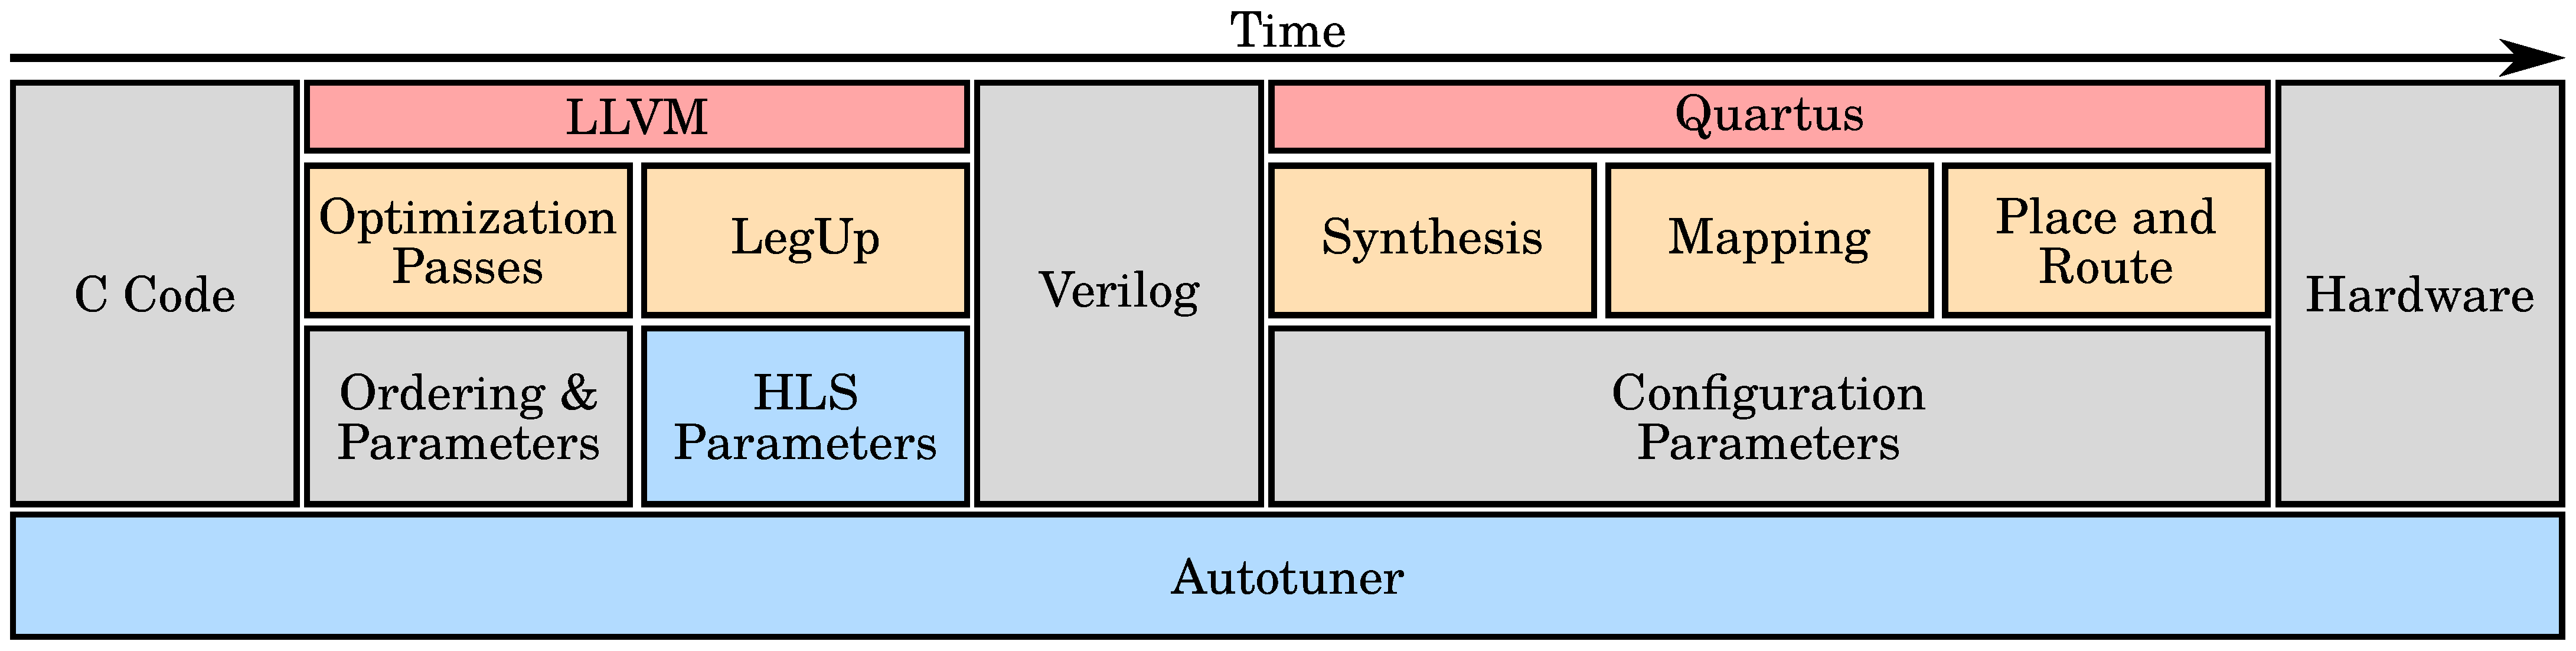
\includegraphics[width=0.8\textwidth]{fpga-stack}
    \caption{High-Level Synthesis compilation process. The autotuner search space at the HLS stage is highlighted in blue}
    \label{fig:fpga-stack}
\end{figure}

Figure \ref{fig:fpga-stack} shows the steps to generate a hardware description
from C code. It also shows the Quartus steps to generate bitstreams from
hardware descriptions and to obtain the hardware metrics we targeted. Our
autotuner used LegUp's HLS parameters as the search space, but it completed the
hardware generation process to obtain metrics from Quartus, as represented by
blue highlights in Figure \ref{fig:fpga-stack}.

\begin{figure}[htpb]
    \centering
    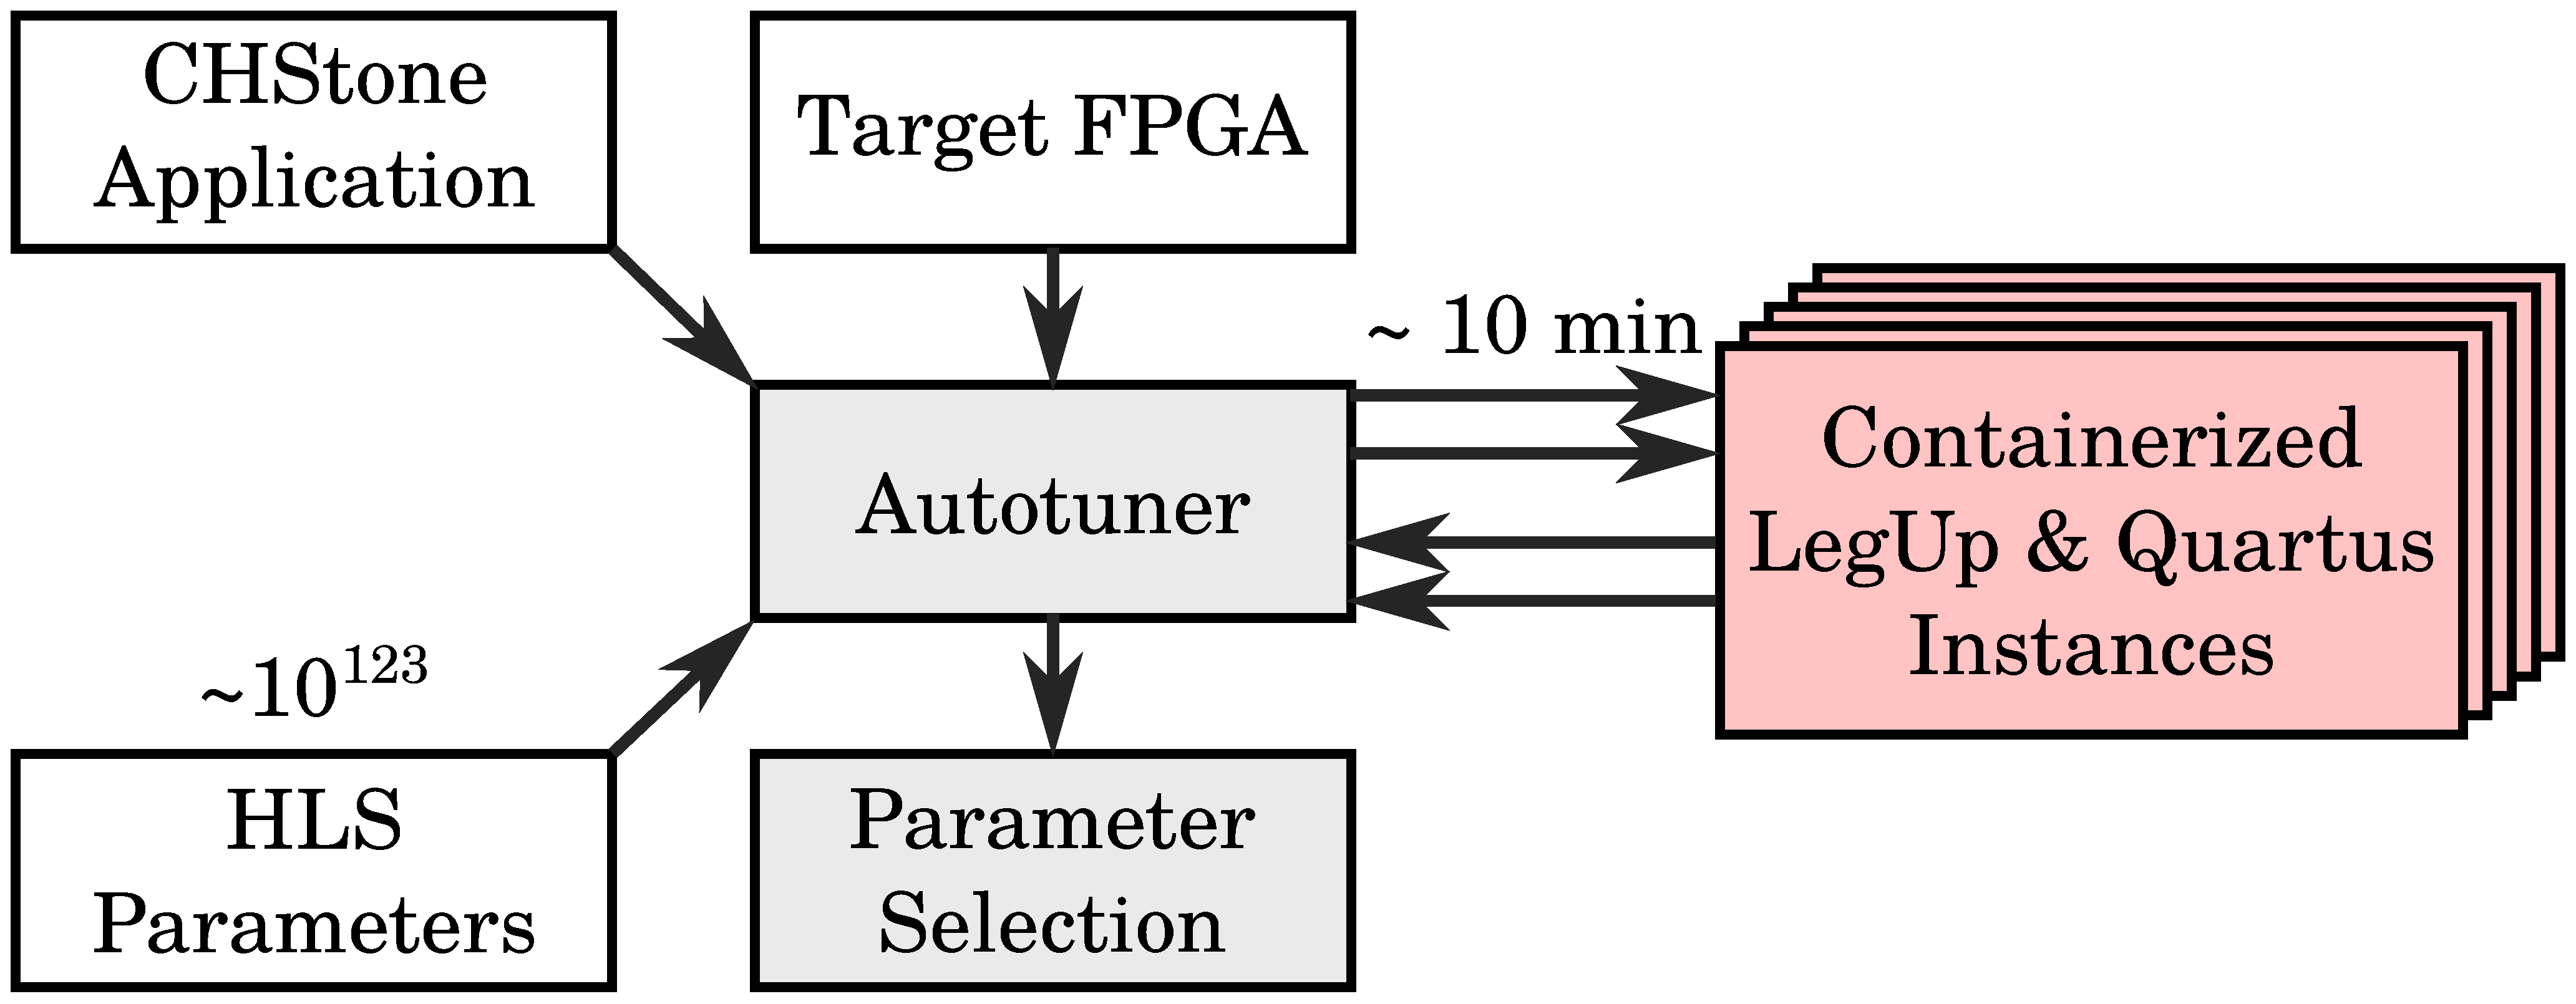
\includegraphics[width=0.6\columnwidth]{fpga_docker_tuner}
    \caption{Autotuner Setup}
    \label{fig:autotuner}
\end{figure}

Figure \ref{fig:autotuner} shows our setup using Docker containers running
LegUp and Quartus. This virtualized setup enabled the portable installation of
dependencies and can be used to run experiments in distributed environments.
The arrows coming from the autotuner to the containers represent the flow of
new configurations generated by search techniques, and the arrows coming from
the containers to the autotuner represent the flow of measurements for a set of
parameters. For CHStone applications the measurement process takes
approximately $10$ minutes to complete, and the majority of this time is spent
in Quartus's synthesis, mapping and place \& route.

\subsubsection{High-Level Synthesis Parameters}

We selected an extensive set of LegUp High-Level Synthesis parameters, shown
partially in Table \ref{tab:params}. Each parameter in the first two rows of
Table \ref{tab:params} has an $8$, $16$, $32$ and $64$ bit variant.
\textit{Operation Latency} parameters define the number of clock cycles
required to complete a given operation when compiled with LegUp.
\textit{Zero-latency} operations can be performed in a single clock cycle.
\textit{Resource Constraint} parameters define the number of times a given
operation can be performed in a clock cycle.  \textit{Boolean or Multi-Valued}
parameters are used to set various advanced configurations. For example, the
\textbf{\texttt{\small{enable\_pattern\_sharing}}} parameter can be set to
enable resource sharing for patterns of computational operators, as is
described by Hadjis \emph{et al.}~\cite{hadjis2012impact}.  For a complete list
and description of each parameter, please refer to LegUp's official
documentation~\footnote{\url{http://legup.eecg.utoronto.ca/docs/4.0} [Accessed
in 18/07/2017]}.

\begin{table}[htpb]
\centering
\begin{tabular}{@{}p{0.10\columnwidth}p{0.84\columnwidth}@{}}
\toprule
Type & \multicolumn{1}{c}{Parameters} \\ \midrule
\parbox[t]{0.10\columnwidth}{\scriptsize{Operation \\ Latency}} & \scriptsize{\texttt{\textbf{altfp\_}[divide, truncate, fptosi, add, subtract, multiply, extend, sitofp], \textbf{unsigned\_}[multiply, divide, add, modulus], \textbf{signed\_}[modulus, divide, multiply, add, \textbf{comp\_}[o, u]], [local\_mem, mem]\textbf{\_dual\_port}, \textbf{reg}}} \\
%\addlinespace{}
\parbox[t]{0.10\columnwidth}{\scriptsize{Resource Constraint}} & \scriptsize{\texttt{\textbf{signed\_}[divide, multiply, modulus, add], \textbf{altfp\_}[multiply, add, subtract, divide], \textbf{unsigned\_}[modulus, multiply, add, divide], [shared\_mem, mem]\textbf{\_dual\_port}}} \\
%\addlinespace{}
\parbox[t]{0.10\columnwidth}{\scriptsize{Boolean~or Multi-value}} & \scriptsize{\texttt{\textbf{pattern\_share\_}[add, shift, sub, bitops], \textbf{sdc\_}[multipump, no\_chaining, priority], \textbf{pipeline\_}[resource\_sharing, all], \textbf{ps\_}[min\_size, min\_width, max\_size, bit\_diff\_threshold], \textbf{mb\_}[minimize\_hw, max\_back\_passes], \textbf{no\_roms}, \textbf{multiplier\_no\_chain}, \textbf{dont\_chain\_get\_elem\_ptr}, \textbf{clock\_period}, \textbf{no\_loop\_pipelining}, \textbf{incremental\_sdc}, \textbf{disable\_reg\_sharing}, \textbf{set\_combine\_basicblock}, \textbf{enable\_pattern\_sharing}, \textbf{multipumping}, \textbf{dual\_port\_binding}, \textbf{modulo\_scheduler}, \textbf{explicit\_lpm\_mults}}} \\ \bottomrule
%%\addlinespace{}
\end{tabular}
\caption{Subset of All Autotuned LegUP HLS Parameters}
\label{tab:params}
\end{table}

\subsubsection{Autotuning Metrics}
\label{sec:metrics}

To obtain values for hardware metrics we needed to perform the synthesis,
mapping and place \& route steps. We used Quartus to do so, and selected 8
hardware metrics reported by Quartus to compose our cost or fitness function.
From the fitter summary we obtained 6 metrics. \textit{Logic Utilization}
(\textit{LUT}) measures the number of logic elements and is composed of
Adaptive Look-Up Table (ALUTs), memory ALUTs, logic registers or dedicated
logic registers.  The \textit{Registers} (\textit{Regs.}), \textit{Virtual
Pins} (\textit{Pins}), \textit{Block Memory Bits} (\textit{Blocks}),
\textit{RAM Blocks} (\textit{BRAM}) and \textit{DSP Blocks} (\textit{DSP})
metrics measure the usage of the resources indicated by their names.

From the timing analysis we obtained the \textit{Cycles} and \textit{FMax}
metrics, used to compute the \textit{Wall-Clock Time} metric. This metric
composed the cost function, but \textit{Cycles} and \textit{FMax} were not
individually used. We chose to do that because all of our hardware metrics
needed to be minimized except for \textit{FMax}, and computing
\textit{Wall-Clock Time} instead solved that restriction.  The
\textit{Wall-Clock Time} $wct$ is computed by $wct = \text{\textit{Cycles}}
\times (\alpha / \text{\textit{FMax}})$, where $\alpha = 10^6$ because
\textit{FMax} is reported in MHz.

Equation \ref{eq:wnsm} describes the cost or fitness function used by our
autotuner to evaluate the sets of HLS parameters generated during tuning.  The
function $f(M, W)$ computes a \textit{Weighted Normalized Sum} (\textbf{WNS})
of the measured metrics $m_i \in M$, where $M$ was described previously.  The
weights $w_i \in W$ correspond to one of the scenarios in Table
\ref{tab:scenarios}. A value is computed for each metric $m_i$ in relation to
an initial value $m_{i}^{0}$ measured for each metric.  For a given set of
measurements $M_t$, a value of $f(M_t, W) = 1.0$ means that there was no
improvement relative to the starting HLS set. The objective of the autotuner is
to minimize $f(M, W)$.

\begin{align} \label{eq:wnsm}
    \mathlarger{f(M, W)} = \frac{\mathlarger{\mathlarger{\mathlarger{\sum}}}\limits_{\substack{m_i \in M \\ w_i \in W}}{w_i\left(\dfrac{m_i}{m_{i}^{0}}\right)}}{\mathlarger{\mathlarger{\mathlarger{\sum}}}\limits_{w_i \in W}{w_i}}
\end{align}

\subsection{Experiments}
\label{sec:FPGAexp}

This section describes the optimization scenarios, the CHStone applications,
and the experimental settings.

\subsubsection{Optimization Scenarios}

Table \ref{tab:scenarios} shows the assigned weights in our $4$ optimization
scenarios. The \textit{Area}-targeting scenario assigns low weights to
wall-clock time metrics. The \textit{Performance \& Latency} scenario assigns
high weights to wall-clock time metrics and also to the number of registers
used.  The \textit{Performance} scenario assigns low weights to area metrics
and cycles, assigning a high weight only to frequency. The balanced scenario
assigns the same weight to every metric. The weights assigned to the metrics
that do not appear on Table \ref{tab:scenarios} are always $1$. The weights are
integers and powers of~$2$.

\begin{table}[htpb]
    \centering
    \begin{tabular}{@{}lcccc@{}}
        \toprule
        Metric & \textit{Area} & \textit{Perf. \& Lat} & \textit{Performance} & \textit{Balanced} \\ \midrule
        \textit{LUT} & \cellcolor[HTML]{9B94B6} High & \cellcolor[HTML]{DD9583} Low & \cellcolor[HTML]{DD9583} Low & \cellcolor[HTML]{E3DBB3} Medium \\
        \textit{Registers} & \cellcolor[HTML]{9B94B6} High & \cellcolor[HTML]{9B94B6} High & \cellcolor[HTML]{E3DBB3} Medium & \cellcolor[HTML]{E3DBB3} Medium \\
        \textit{BRAMs} & \cellcolor[HTML]{9B94B6} High & \cellcolor[HTML]{DD9583} Low & \cellcolor[HTML]{DD9583} Low & \cellcolor[HTML]{E3DBB3} Medium \\
        \textit{DSPs} & \cellcolor[HTML]{9B94B6} High & \cellcolor[HTML]{DD9583} Low & \cellcolor[HTML]{DD9583} Low & \cellcolor[HTML]{E3DBB3} Medium \\
        \textit{FMax} & \cellcolor[HTML]{DD9583} Low & \cellcolor[HTML]{9B94B6} High & \cellcolor[HTML]{9B94B6} High & \cellcolor[HTML]{E3DBB3} Medium \\
        \textit{Cycles} & \cellcolor[HTML]{DD9583} Low & \cellcolor[HTML]{9B94B6} High & \cellcolor[HTML]{DD9583} Low & \cellcolor[HTML]{E3DBB3} Medium \\ \bottomrule
    \end{tabular}
    \caption{Weights for Optimization Scenarios \\ (\textit{High} $= 8$, \textit{Medium} $= 4$, \textit{Low} $= 2$)}
    \label{tab:scenarios}
    %\addlinespace
\end{table}

We compared results when starting from a \textit{default} configuration with
the results when starting at a \textit{random} set of parameters. The default
configuration for the StratixV was provided by LegUp and the comparison was
performed in the \textit{Balanced} optimization scenario.

\subsubsection{Applications}

To test and validate our autotuner we used 11 applications from the CHStone HLS
benchmark suite~\cite{hara2008chstone}. CHStone applications are implemented in
the C language and contain inputs and previously computed outputs, allowing for
correctness checks to be performed for all applications.

\begin{table}[htpb]
\centering
\begin{tabular}{@{}p{0.13\columnwidth}p{0.63\columnwidth}@{}}
\toprule
 Application & Short Description \\ \midrule
 blowfish & Symmetric-key block cypher \\
 aes & Advanced Encryption Algorithm (AES) \\
 adpcm & Adaptive Differential Pulse Code Modulation dec. and enc. \\
 sha & Secure Hash Algorithm (SHA) \\
 motion & Motion vector decoding from MPEG-2 \\
 mips & Simplified MIPS processor \\
 gsm & Predictive coding analysis of systems for mobile comms. \\
 dfsin & Sine function for double-precision floating-point numbers \\
 dfmul & Double-precision floating-point multiplication \\
 dfdiv & Double-precision floating-point division \\
 dfadd & Double-precision floating-point addition \\ \bottomrule
%% \addlinespace{}
\end{tabular}
\caption{Autotuned CHStone Applications}
\label{tab:chstone}
\end{table}

Table \ref{tab:chstone} provides short descriptions of the $11$ CHStone
applications we used. We were not able to compile the \textit{jpeg} CHStone
application, so did not use it.  All experiments targeted the \textit{Intel
StratixV 5SGXEA7N2F45C2} FPGA.

\subsubsection{Experiments}

We performed $10$ tuning runs of $1.5h$ for each application.  Section
\ref{sec:FPGAresults} presents the mean relative improvements for each application
and individual metric. The code needed to run the experiments and generate the
figures, as well as the implementation of the autotuner and all data we
generated, is open and hosted at
GitHub~\footnote{\url{https://github.com/phrb/legup-tuner} [Accessed in
18/07/2017]}.

The experimental settings included Docker for virtualization and
reproducibility, LegUp $v4.0$, Quartus Prime Standard Edition $v16.0$, and
CHStone. All experiments were performed on a machine with two Intel(R) Xeon(R)
CPU E5-2699 v3 with 18 x86\_64 cores each, and 503GB of RAM.  The instructions
and the code to reproduce the software experimental environment are open and
hosted at GitHub~\footnote{\url{https://github.com/phrb/legup-dockerfile}
[Accessed in 18/07/2017]}.

\subsection{Results}
\label{sec:FPGAresults}

This section presents summaries of the results from $10$ autotuning runs of
$1.5h$ in the scenarios from Table \ref{tab:scenarios}.  Results are presented
in \textit{heatmaps} where each row has one of the 11 CHStone applications in
Table \ref{tab:chstone} and each column has one of the 8 hardware metrics and
their \textit{Weighted Normalized Sum} (\textbf{WNS}) as described in Section
\ref{sec:metrics}.

Cells on heatmaps show the ratio of tuned to initial values of a hardware
metric in a CHStone application, averaged over 10 autotuning runs. The
objective of the autotuner is to minimize all hardware metrics except for
\textit{FMax}.  To create a consistent presentation of our data in the heatmaps
we inverted the ratios for \textit{FMax} so that cell values less than $1.0$
always mean a better metric value.  Heatmaps are also colored so that darker
blues mean better values and darker reds mean worse values in relation to the
starting point.

\begin{figure}[htpb]
    \centering
    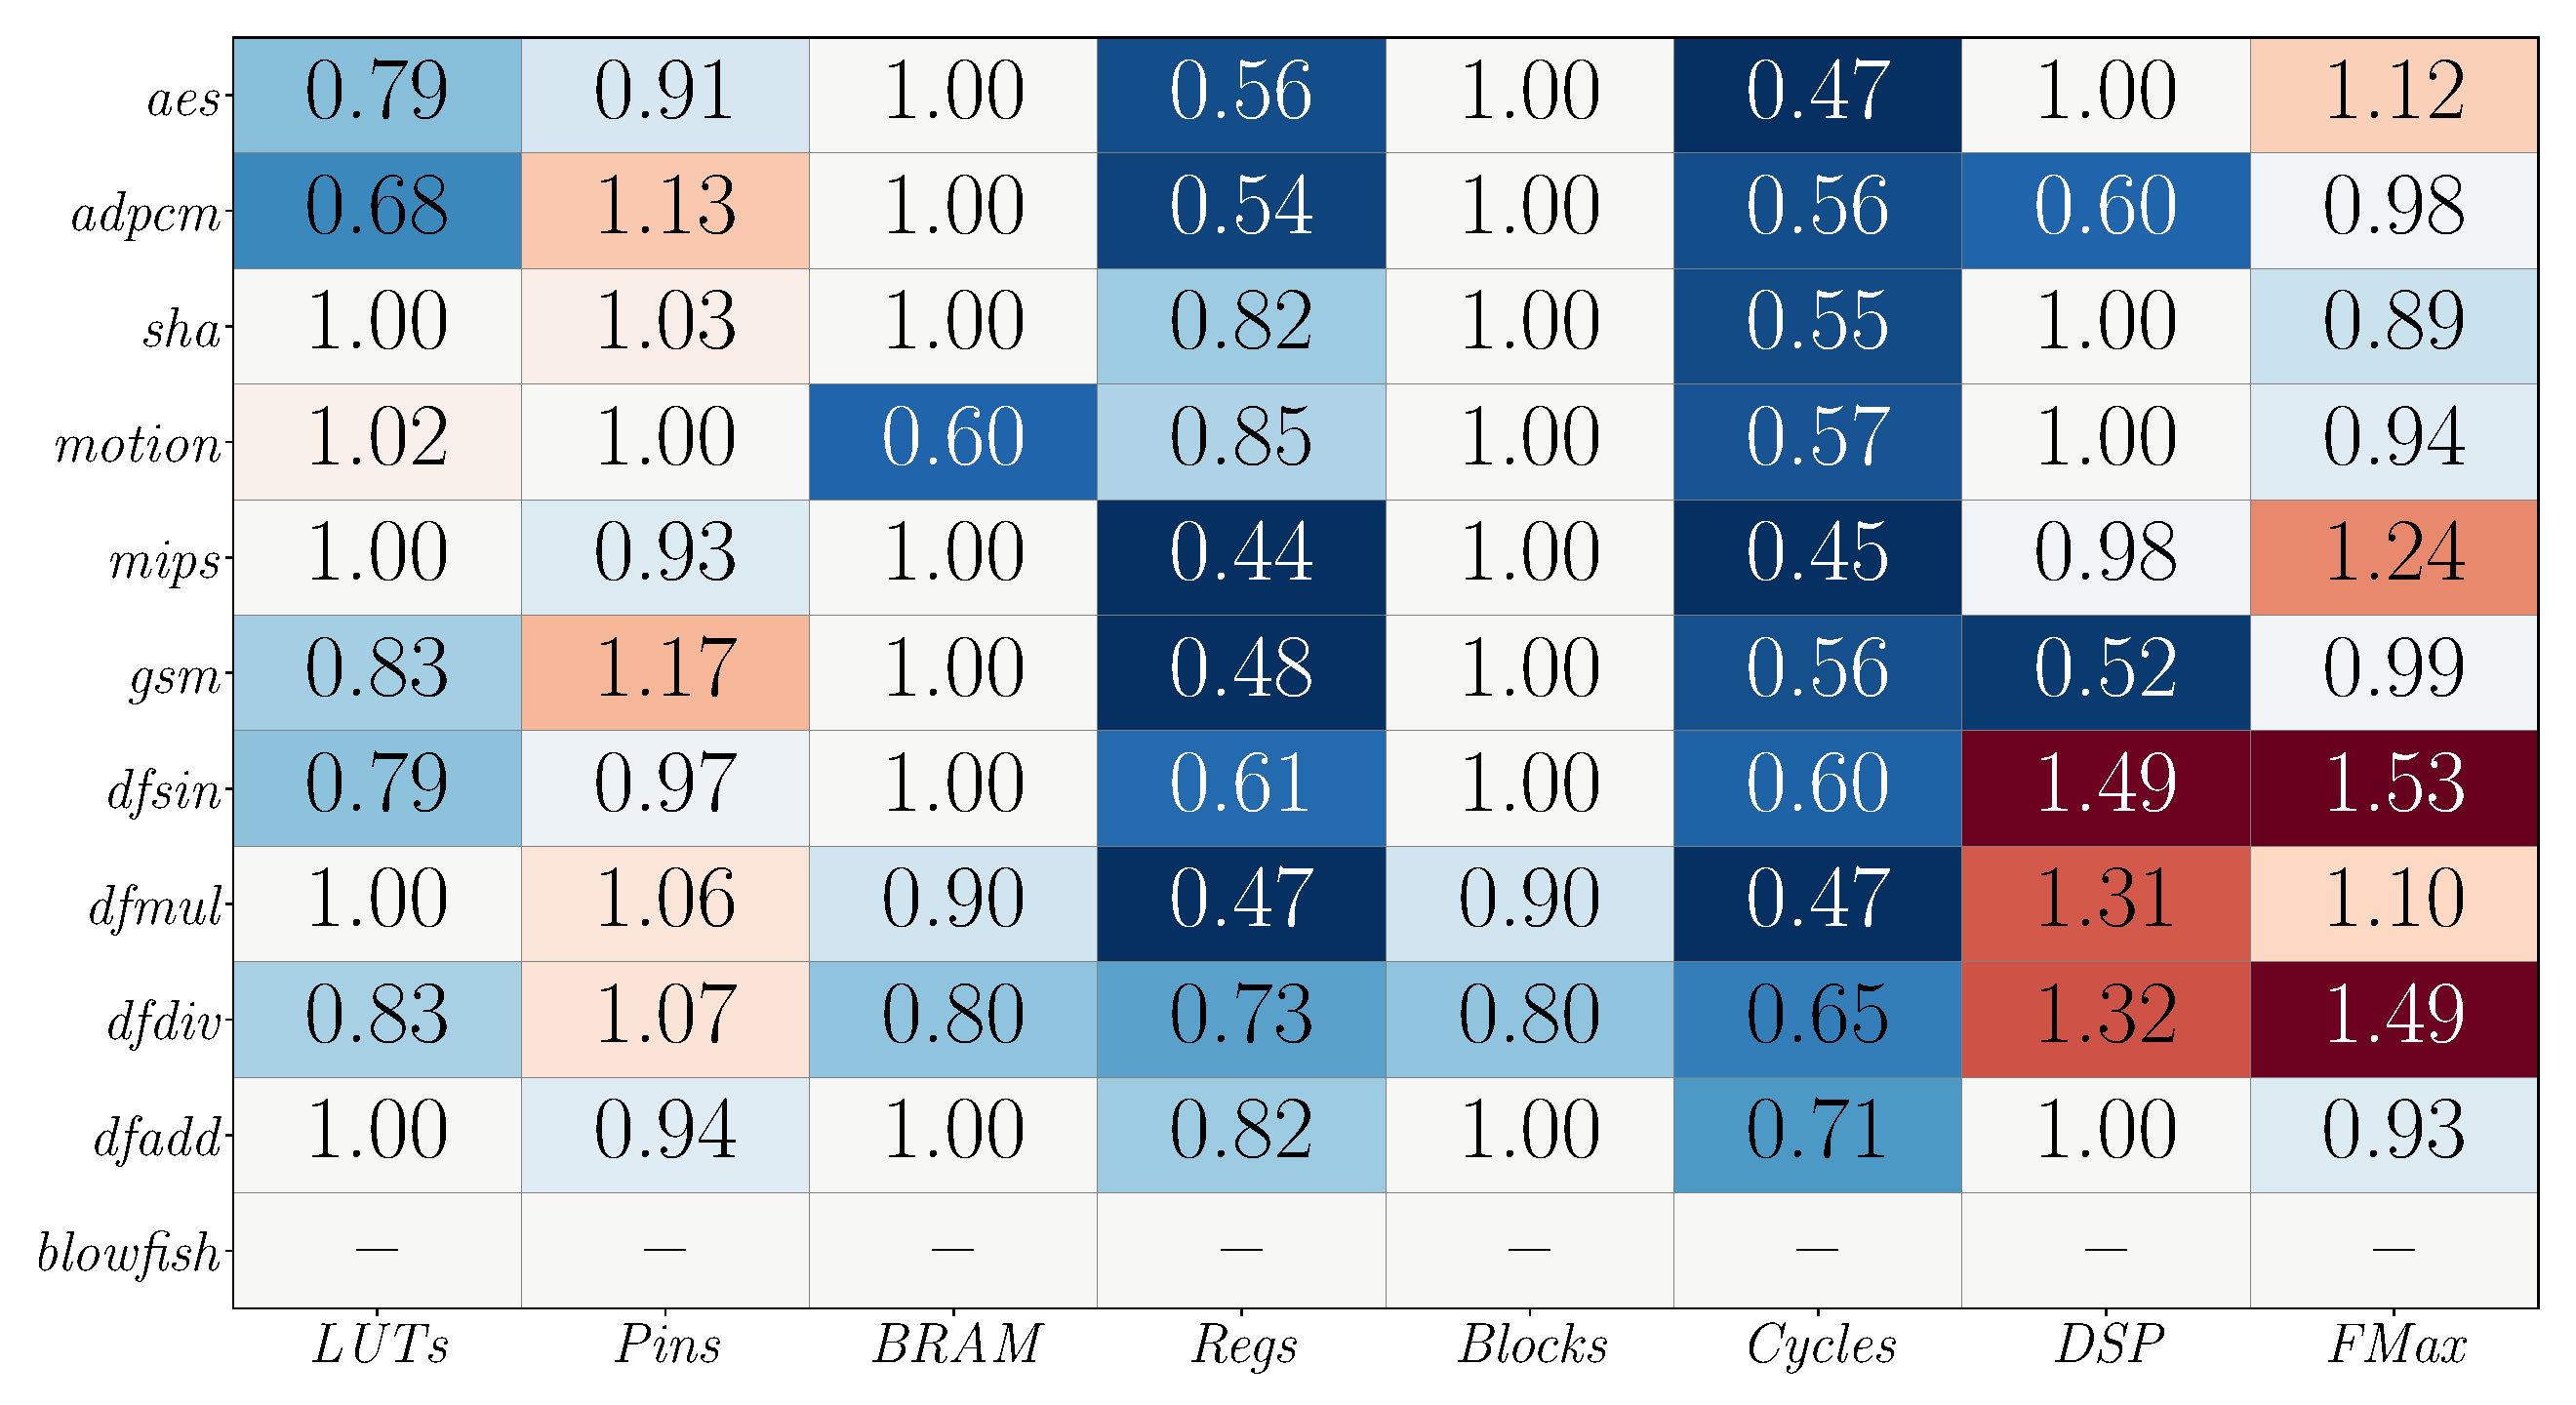
\includegraphics[width=0.5\columnwidth]{heatmap_comp_stratixV}
    \caption{Comparison of the absolute values for Random and Default starting points in the Balanced scenario}
    \label{fig:comp}
\end{figure}

Figure \ref{fig:comp} compares the ratios of absolute values for each hardware
metric for \textit{Default} and \textit{Random} starts, in the
\textit{Balanced} scenario.  Cell values less than $1.0$ mean that the
\textit{Default} start achieved smaller absolute values that the
\textit{Random} start.  Values of ``--'' mean that the \textit{Default} start
could not find a set of HLS parameters that produced a valid output during any
of the $1.5h$ tuning runs. The \textit{Default} start found better values for
most metrics.

The \textit{Random} start found better values for \textit{DSP}, \textit{Pins}
and \textit{FMax} for some applications. For example, it found values $49\%$
smaller, $6\%$ smaller and $53\%$ larger for \textit{DSP}, \textit{Pins} and
\textit{FMax}, respectively, for the \textit{dfsin} application. The
\textit{Default} start found better values for \textit{Regs} and
\textit{Cycles} for all applications. For example, it found values $53\%$
smaller for \textit{Regs} and \textit{Cycles} for the \textit{dfmul}
application, and $56\%$ and $55\%$ smaller for \textit{Regs} and
\textit{Cycles}, respectively, for the \textit{mips} application.

We believe that the \textit{Random} start found worst values in most cases
because of the size of the search space. It is important that autotuners use
default starting points specific to a given application and board.  The
remaining results in this Section used the \textit{Default} starting point
provided by LegUp.

Figure \ref{fig:balanced} shows the results for the \textit{Balanced} scenario.
These results are the baseline for evaluating the autotuner in other scenarios,
since all metrics had the same weight.  The optimization target was the
\textit{Weighted Normalized Sum} (\textbf{WNS}) of hardware metrics, but we
were also interested in the changes in other metrics as their relative weights
changed. In the \textit{Balanced} scenario we expected to see smaller
improvements of \textbf{WNS} due to the competition of concurrent improvements
on every metric.

The autotuner found values of \textbf{WNS} $16\%$ smaller for \textit{adpcm}
and \textit{dfdiv}, and $15\%$ smaller for \textit{dfmul}.  Even on the
\textit{Balanced} scenario it is possible to see that some metrics decreased
while others decreased consistently over the 10 tuning runs. \textit{FMax} and
\textit{DSP} had the larger improvements for most applications, for example,
$51\%$ greater \textit{FMax} in \textit{adpcm} and $69\%$ smaller \textit{DSP}
in \textit{dfmul}.  \textit{Cycles}, \textit{Regs} and \textit{Pins} had the
worst results in this scenario, with $34\%$ larger \textit{Cycles} in
\textit{dfdiv}, $15\%$ larger \textit{Regs} in \textit{dfdiv} and $17\%$ larger
\textit{Pins} in \textit{gsm}.  Other metrics had smaller improvements or no
improvements at all in most applications.

\begin{figure}[htpb]
    \begin{minipage}{.48\textwidth}
        \centering
        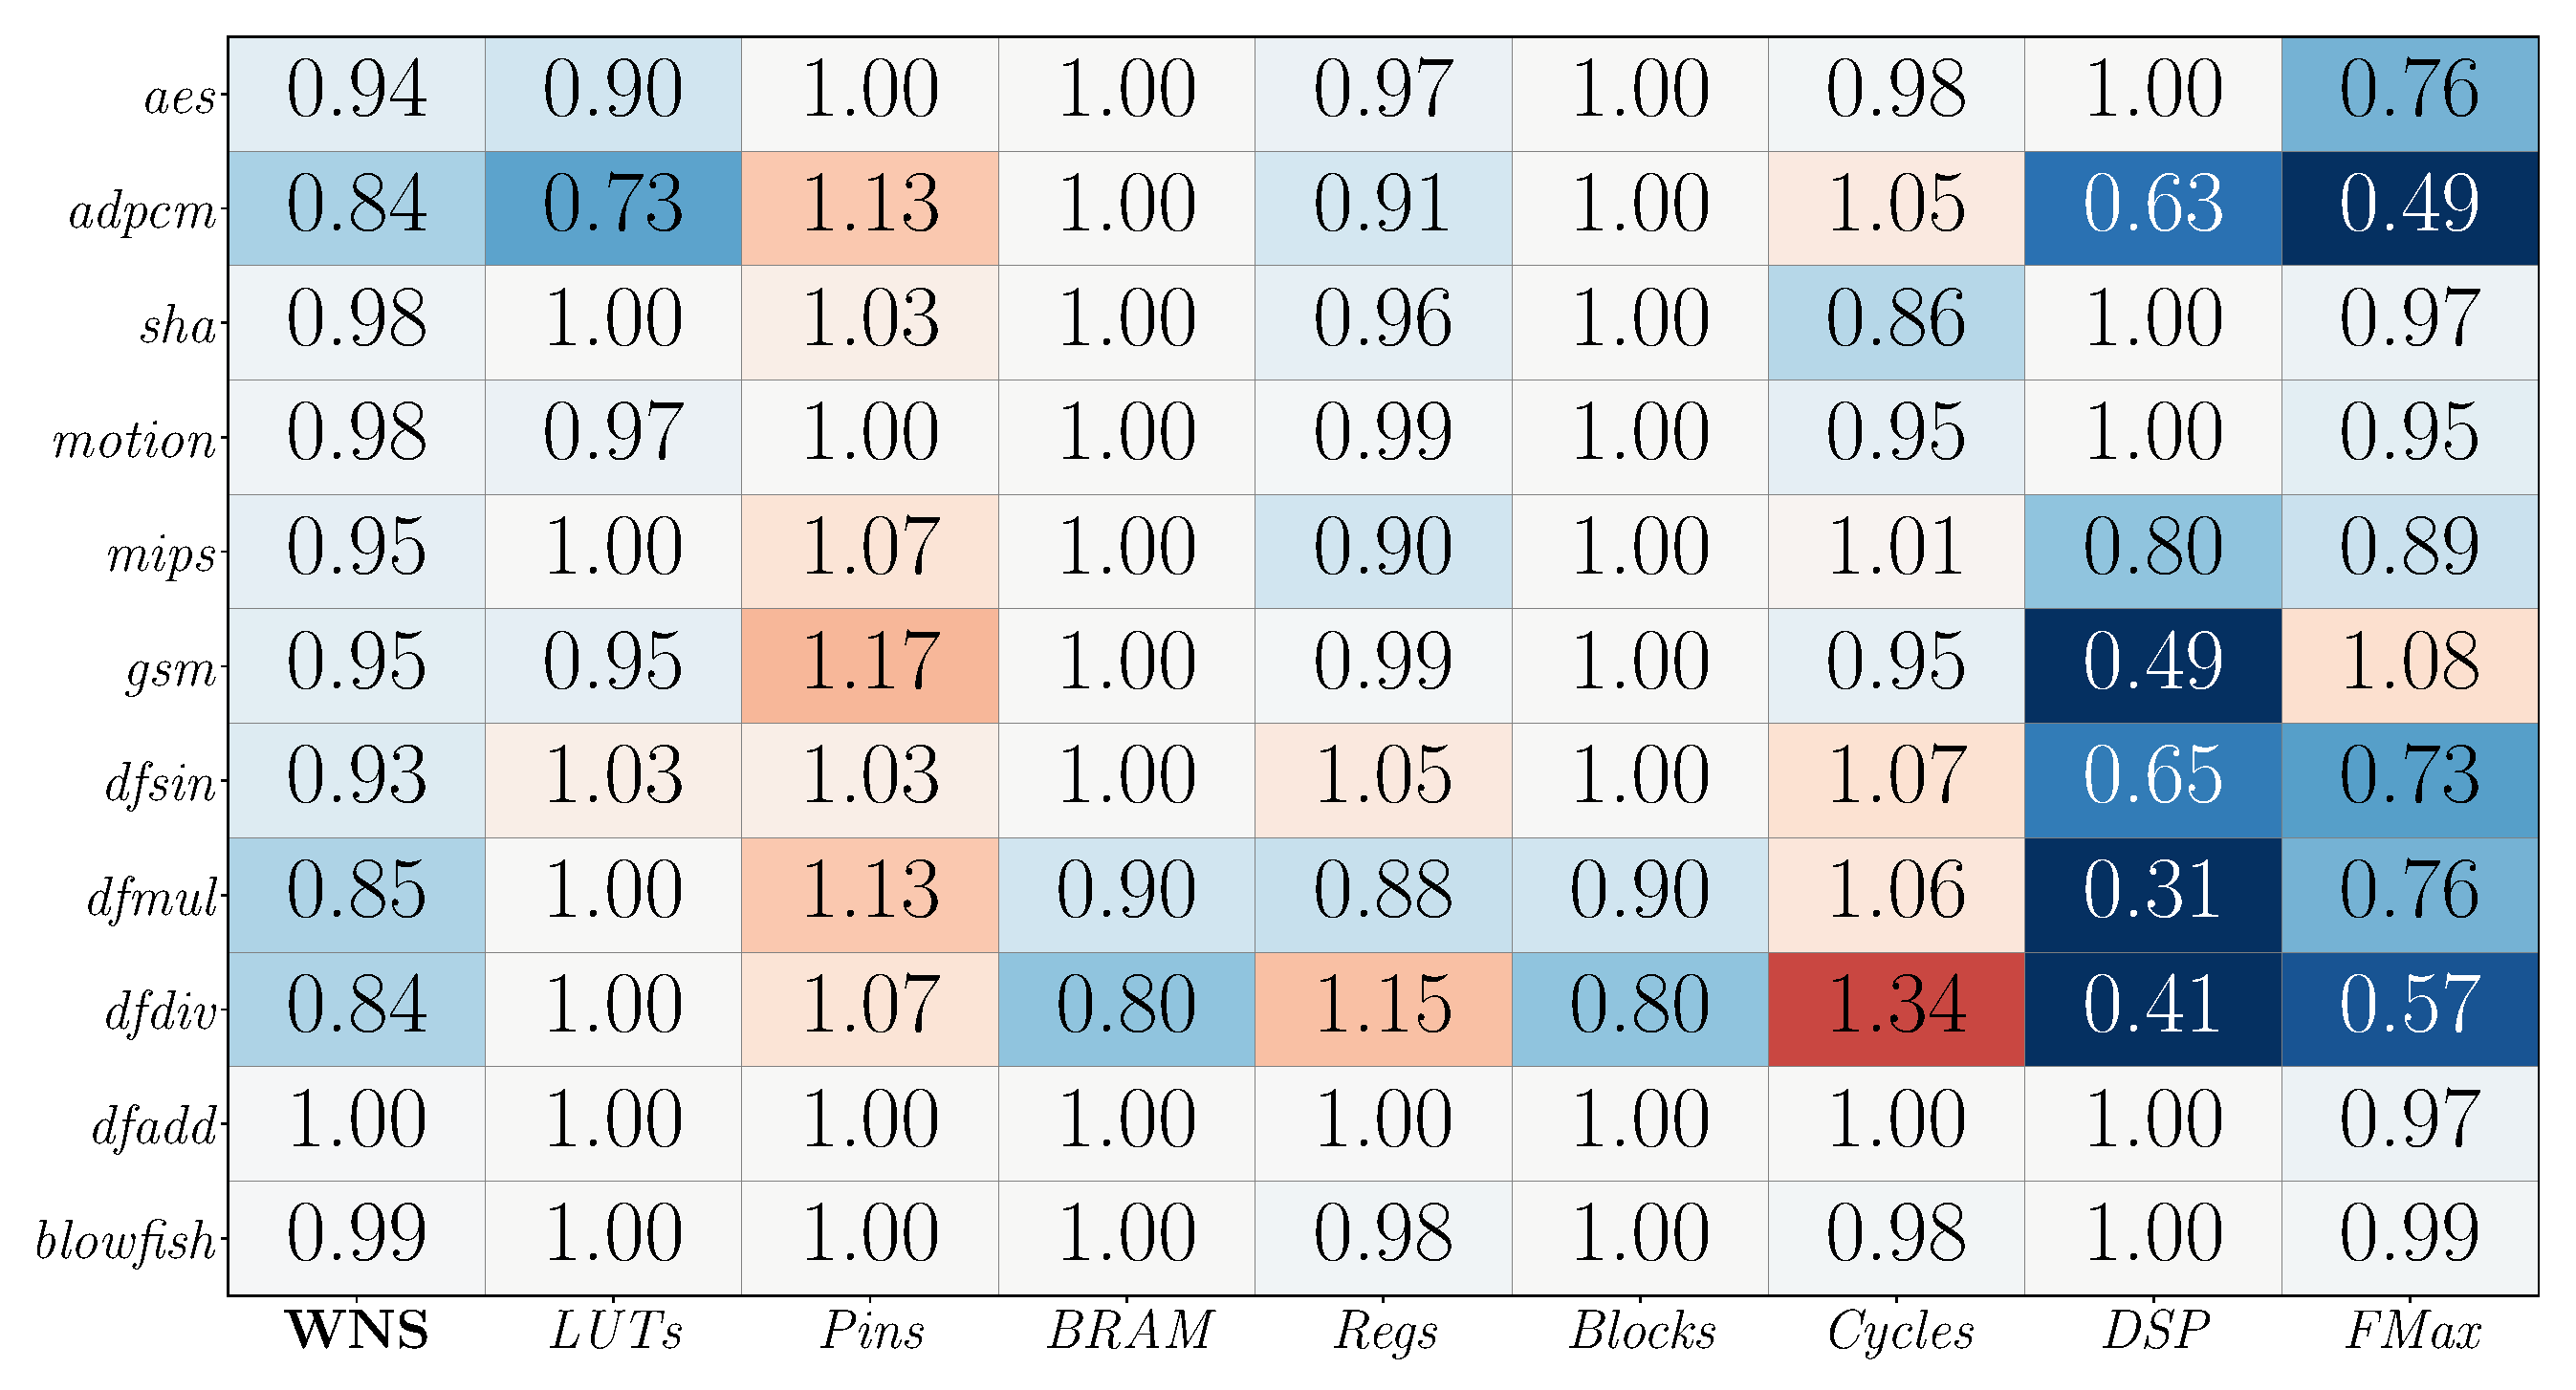
\includegraphics[width=\columnwidth]{heatmap_default_stratixV}
        \caption{Relative improvement for all metrics in the \textit{Balanced}
        scenario}
        \label{fig:balanced}
    \end{minipage}%
    \hfill
    \begin{minipage}{.48\textwidth}
        \centering
        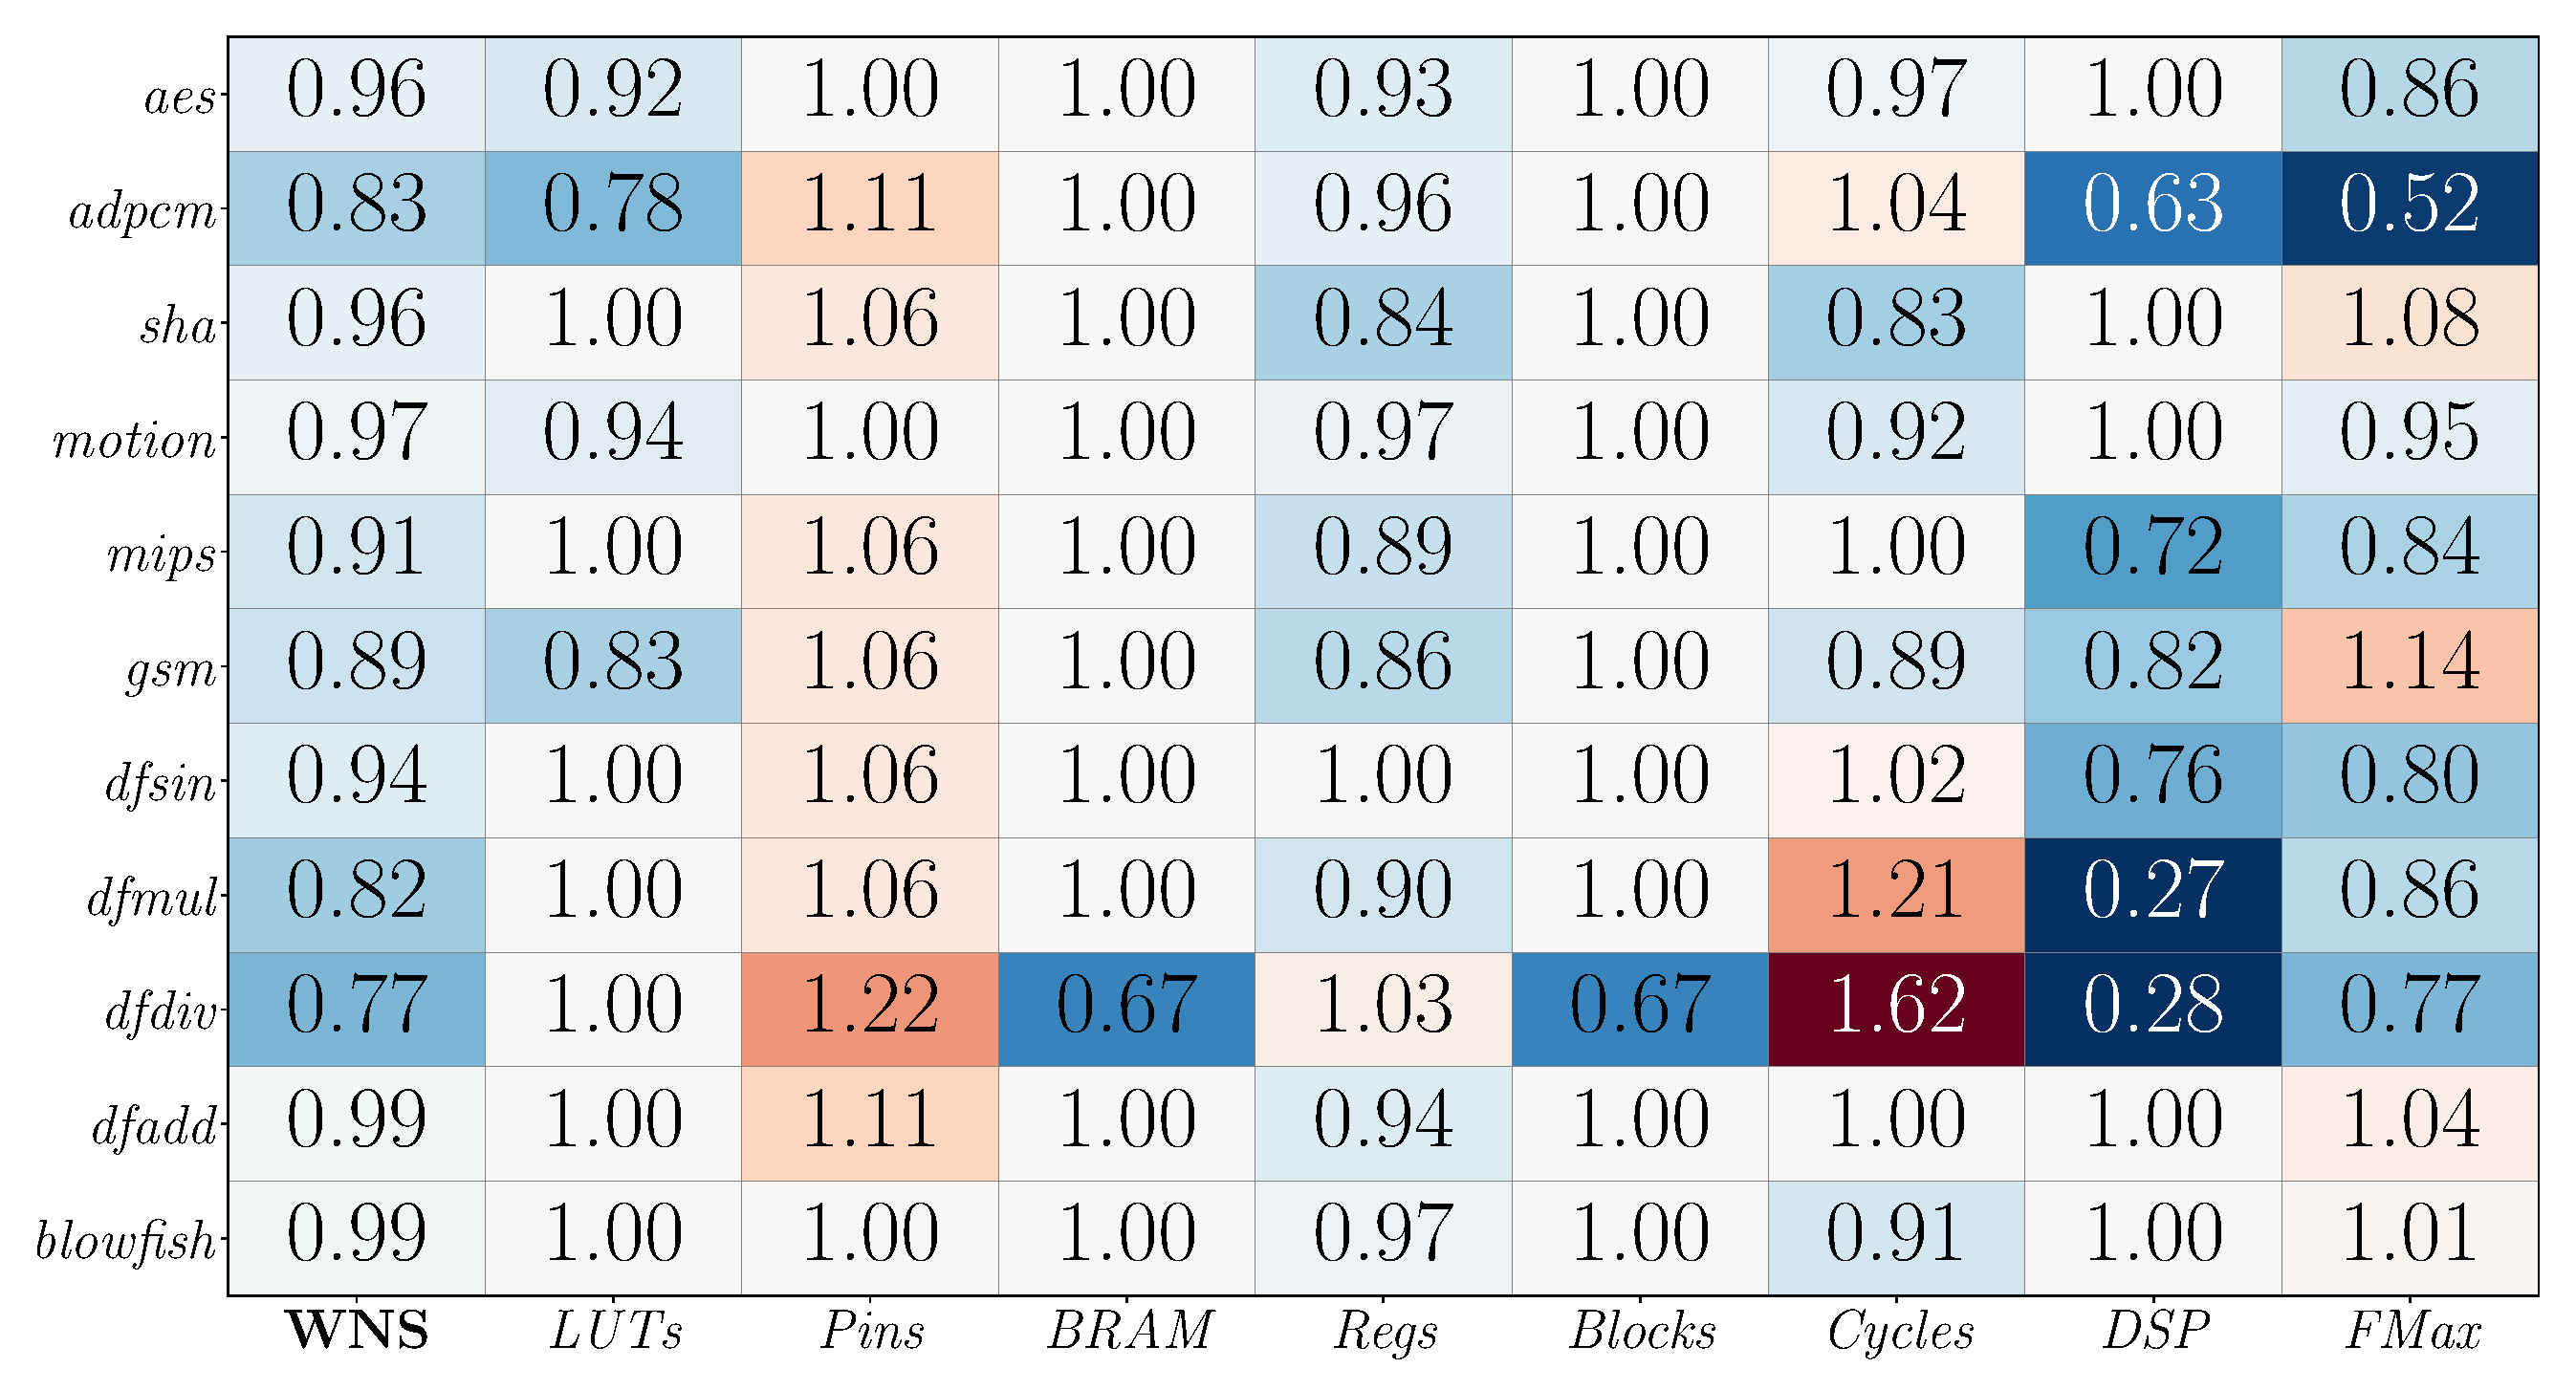
\includegraphics[width=\columnwidth]{heatmap_default_stratixV_area}
        \caption{Relative improvement for all metrics in the \textit{Area}
        scenario}
        \label{fig:area}
    \end{minipage}%
\end{figure}

Figure \ref{fig:area} shows the results for the \textit{Area} scenario.  We
believe that the greater coherence of optimization objectives is responsible
for the greater improvements of \textbf{WNS} in the following scenarios. The
autotuner found values of \textbf{WNS} $23\%$ smaller for \textit{dfdiv},
$18\%$ smaller for \textit{dfmul}, and smaller values overall in comparison
with the \textit{Balanced} scenario. Regarding individual metrics, the values
for \textit{FMax} were worse overall, with $14\%$ smaller \textit{FMax} in
\textit{gsm} and $62\%$ greater \textit{Cycles}, for example. As expected for
this scenario, metrics related to area had better improvements than in the
\textit{Balanced} scenario, with $73\%$ and $72\%$ smaller \textit{DSP} for
\textit{dfmul} and \textit{dfdiv} respectively, $33\%$ smaller \textit{Blocks}
and \textit{BRAM} in \textit{dfdiv} and smaller values overall for
\textit{Regs} and \textit{LUTs}.

Figure \ref{fig:perf} shows the results for the \textit{Performance} scenario.
The autotuner found values of \textbf{WNS} $23\%$ smaller for \textit{dfmul},
$19\%$ smaller for \textit{dfdiv}, and smaller values overall than in the
\textit{Balanced} scenario.  \textit{FMax} was the only metric with a
\textit{High} weight in this scenario, so most metrics had improvements close
overall to the \textit{Balanced} scenario.  The values for \textit{FMax} were
best overall, with better improvements in most applications. For example,
$41\%$, $30\%$, $44\%$ and $37\%$ greater \textit{FMax} in \textit{dfdiv},
\textit{dfmul}, \textit{dfsin} and \textit{aes} respectively.

\begin{figure}[htpb]
    \centering
    \begin{minipage}{.48\textwidth}
        \centering
        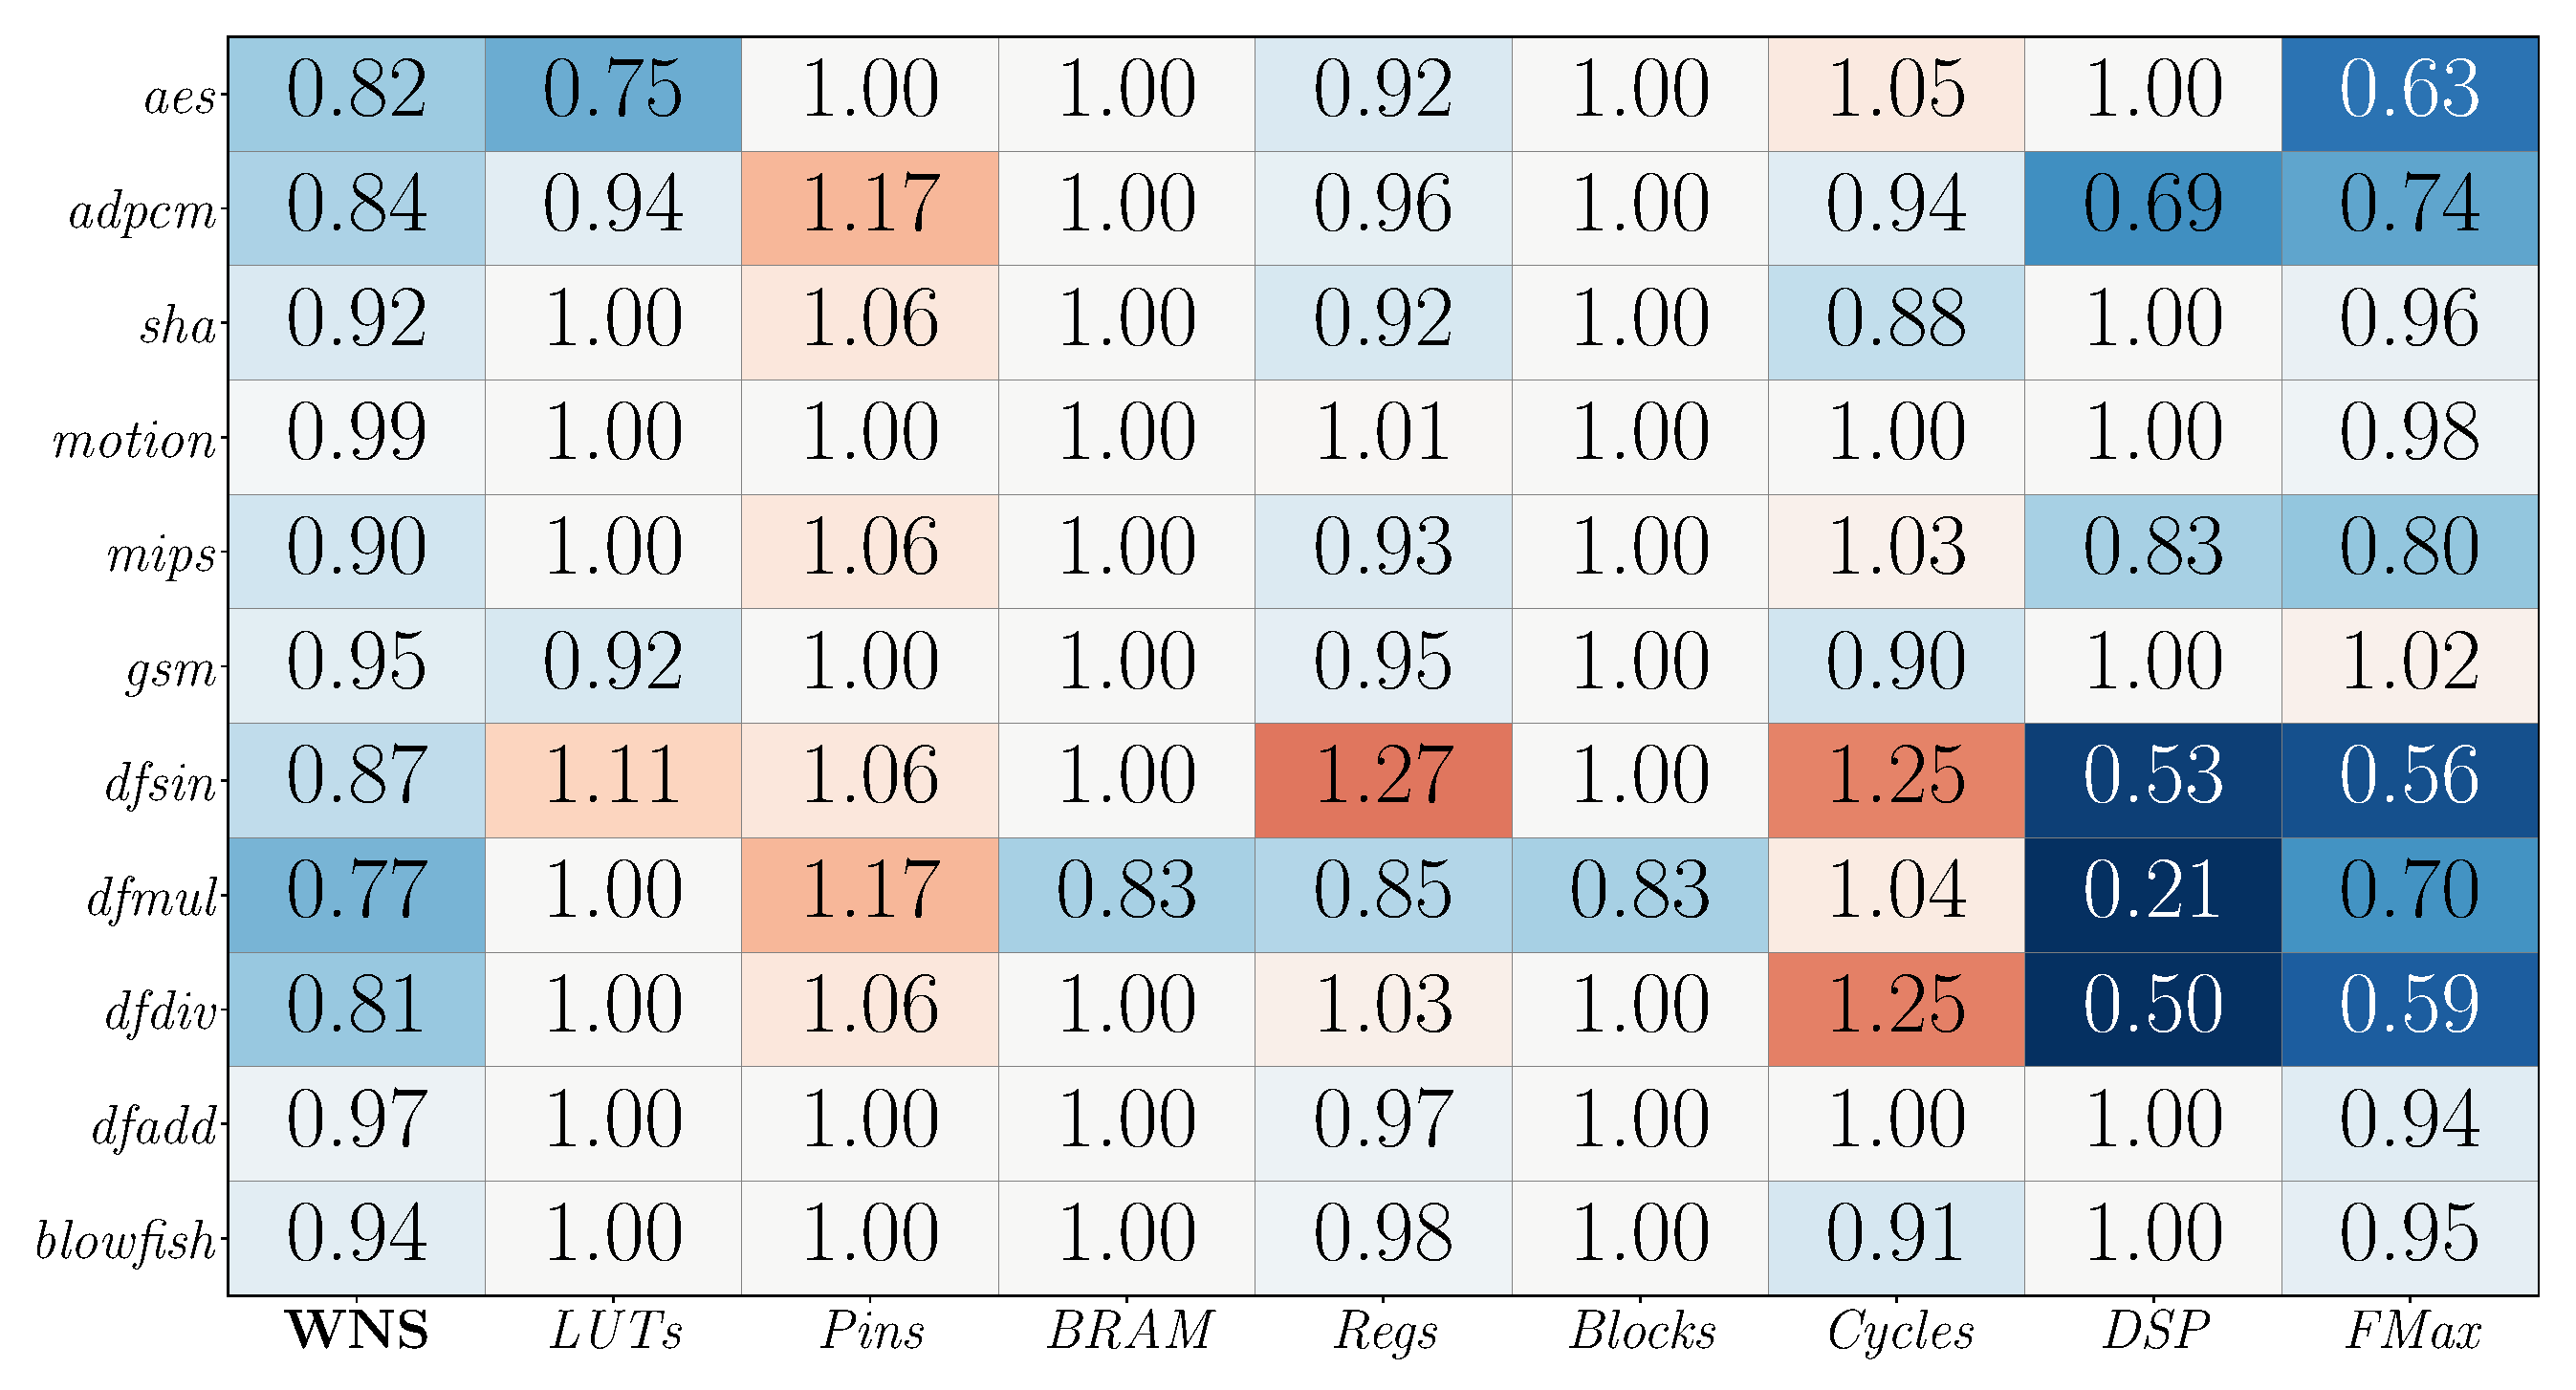
\includegraphics[width=\columnwidth]{heatmap_default_stratixV_perf}
        \caption{Relative improvement for all metrics in the
        \textit{Performance} scenario}
        \label{fig:perf}
    \end{minipage}%
    \hfill
    \begin{minipage}{.48\textwidth}
        \centering
        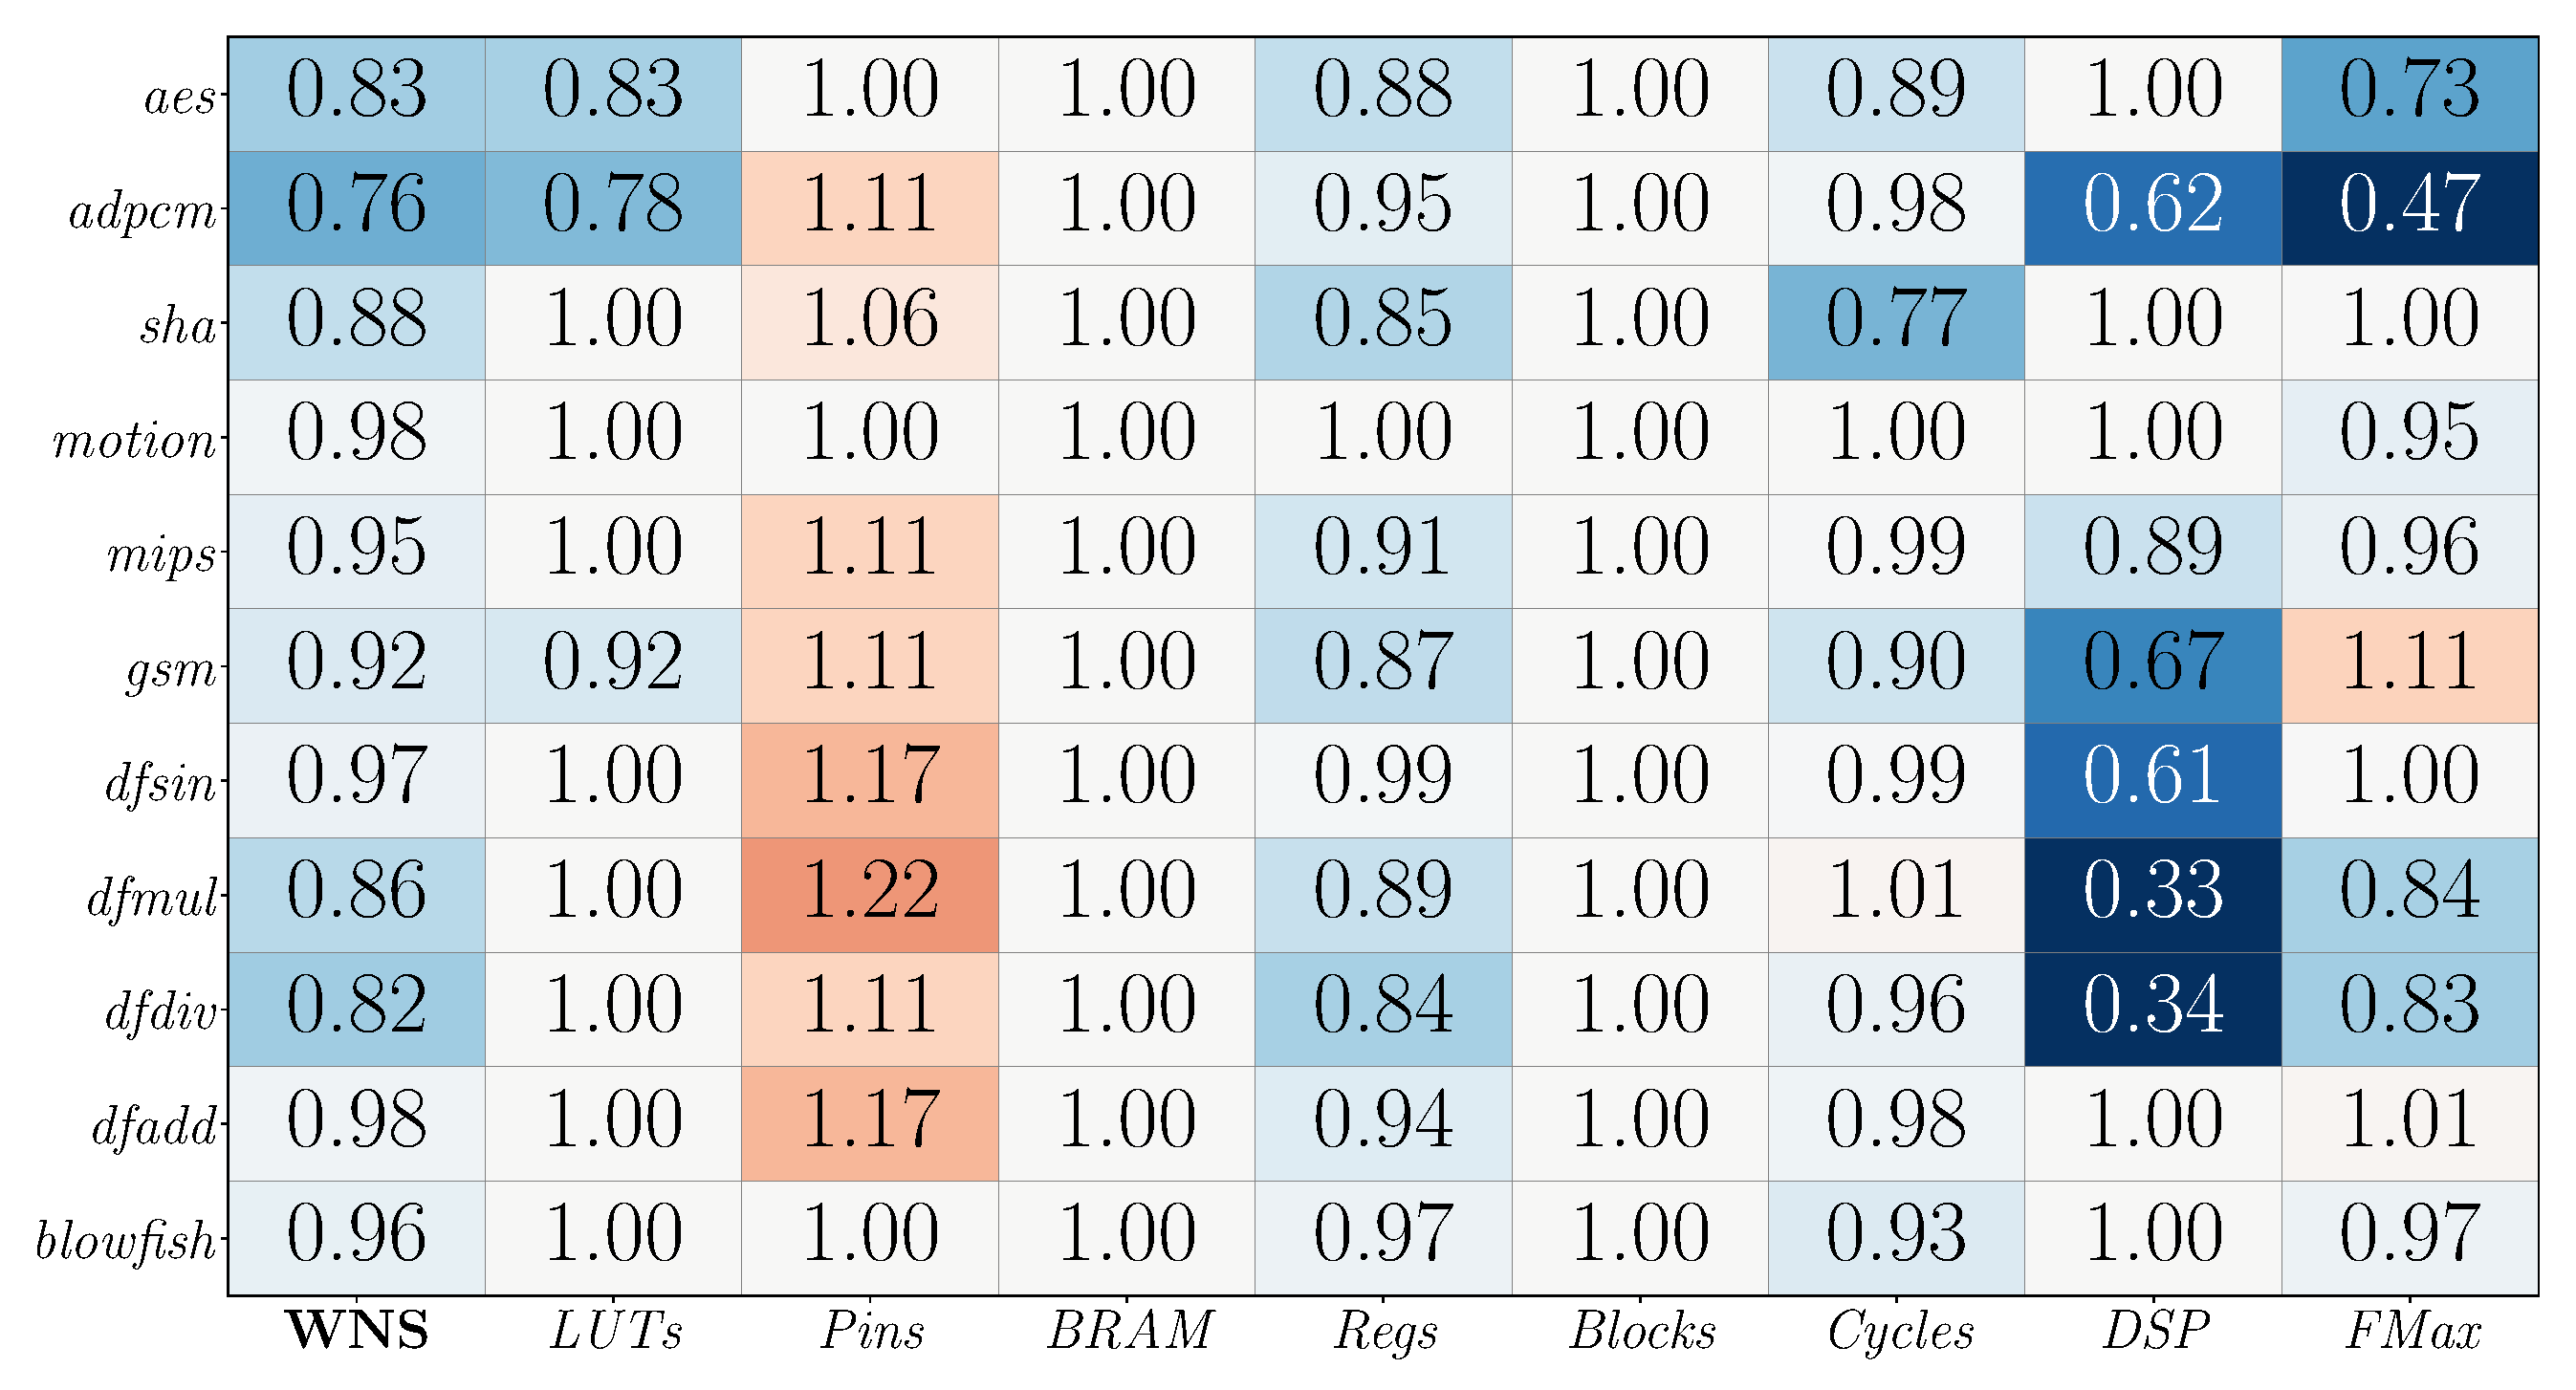
\includegraphics[width=\columnwidth]{heatmap_default_stratixV_perflat}
        \caption{Relative improvement for all metrics in the
        \textit{Performance \& Latency} scenario}
        \label{fig:perflat}
    \end{minipage}
\end{figure}

Figure \ref{fig:perflat} shows the results for the \textit{Performance \&
Latency} scenario.  The autotuner found values of \textbf{WNS} $24\%$ smaller
for \textit{adpcm}, $18\%$ smaller for \textit{dfdiv}, and smaller values
overall than in the \textit{Balanced} scenario. \textit{Regs}, \textit{Cycles}
and \textit{FMax} had higher weights in this scenario, and also better
improvements overall.  For example, $16\%$ and $15\%$ smaller \textit{Regs} in
\textit{dfdiv} and \textit{sha} respectively, $23\%$ and $11\%$ smaller
\textit{Cycles} in \textit{sha} and \textit{aes} respectively, and $53\%$
greater \textit{FMax} in \textit{adpcm}. Although \textit{FMax} had the worst
improvements in relation to the \textit{Balanced} scenario, the
\textit{Wall-Clock Time} was still decreased by the smaller values of
\textit{Cycles}.

Figure \ref{fig:wns-comp} summarizes the average improvements on \textbf{WNS}
in the 4 scenarios over 10 runs. Only the \textit{Weighted Normalized Sum} of
metrics directly guided optimization. With the exception of \textit{dfadd} in
the \textit{Balanced} scenario, the autotuner decreased \textbf{WNS} for all
applications in all scenarios by $10\%$ on average, and up to $24\%$ for
\textit{adpcm} in the \textit{Performance \& Latency} scenario. The figure also
shows the average decreases for each scenario.

\begin{figure}[htpb]
    \centering
    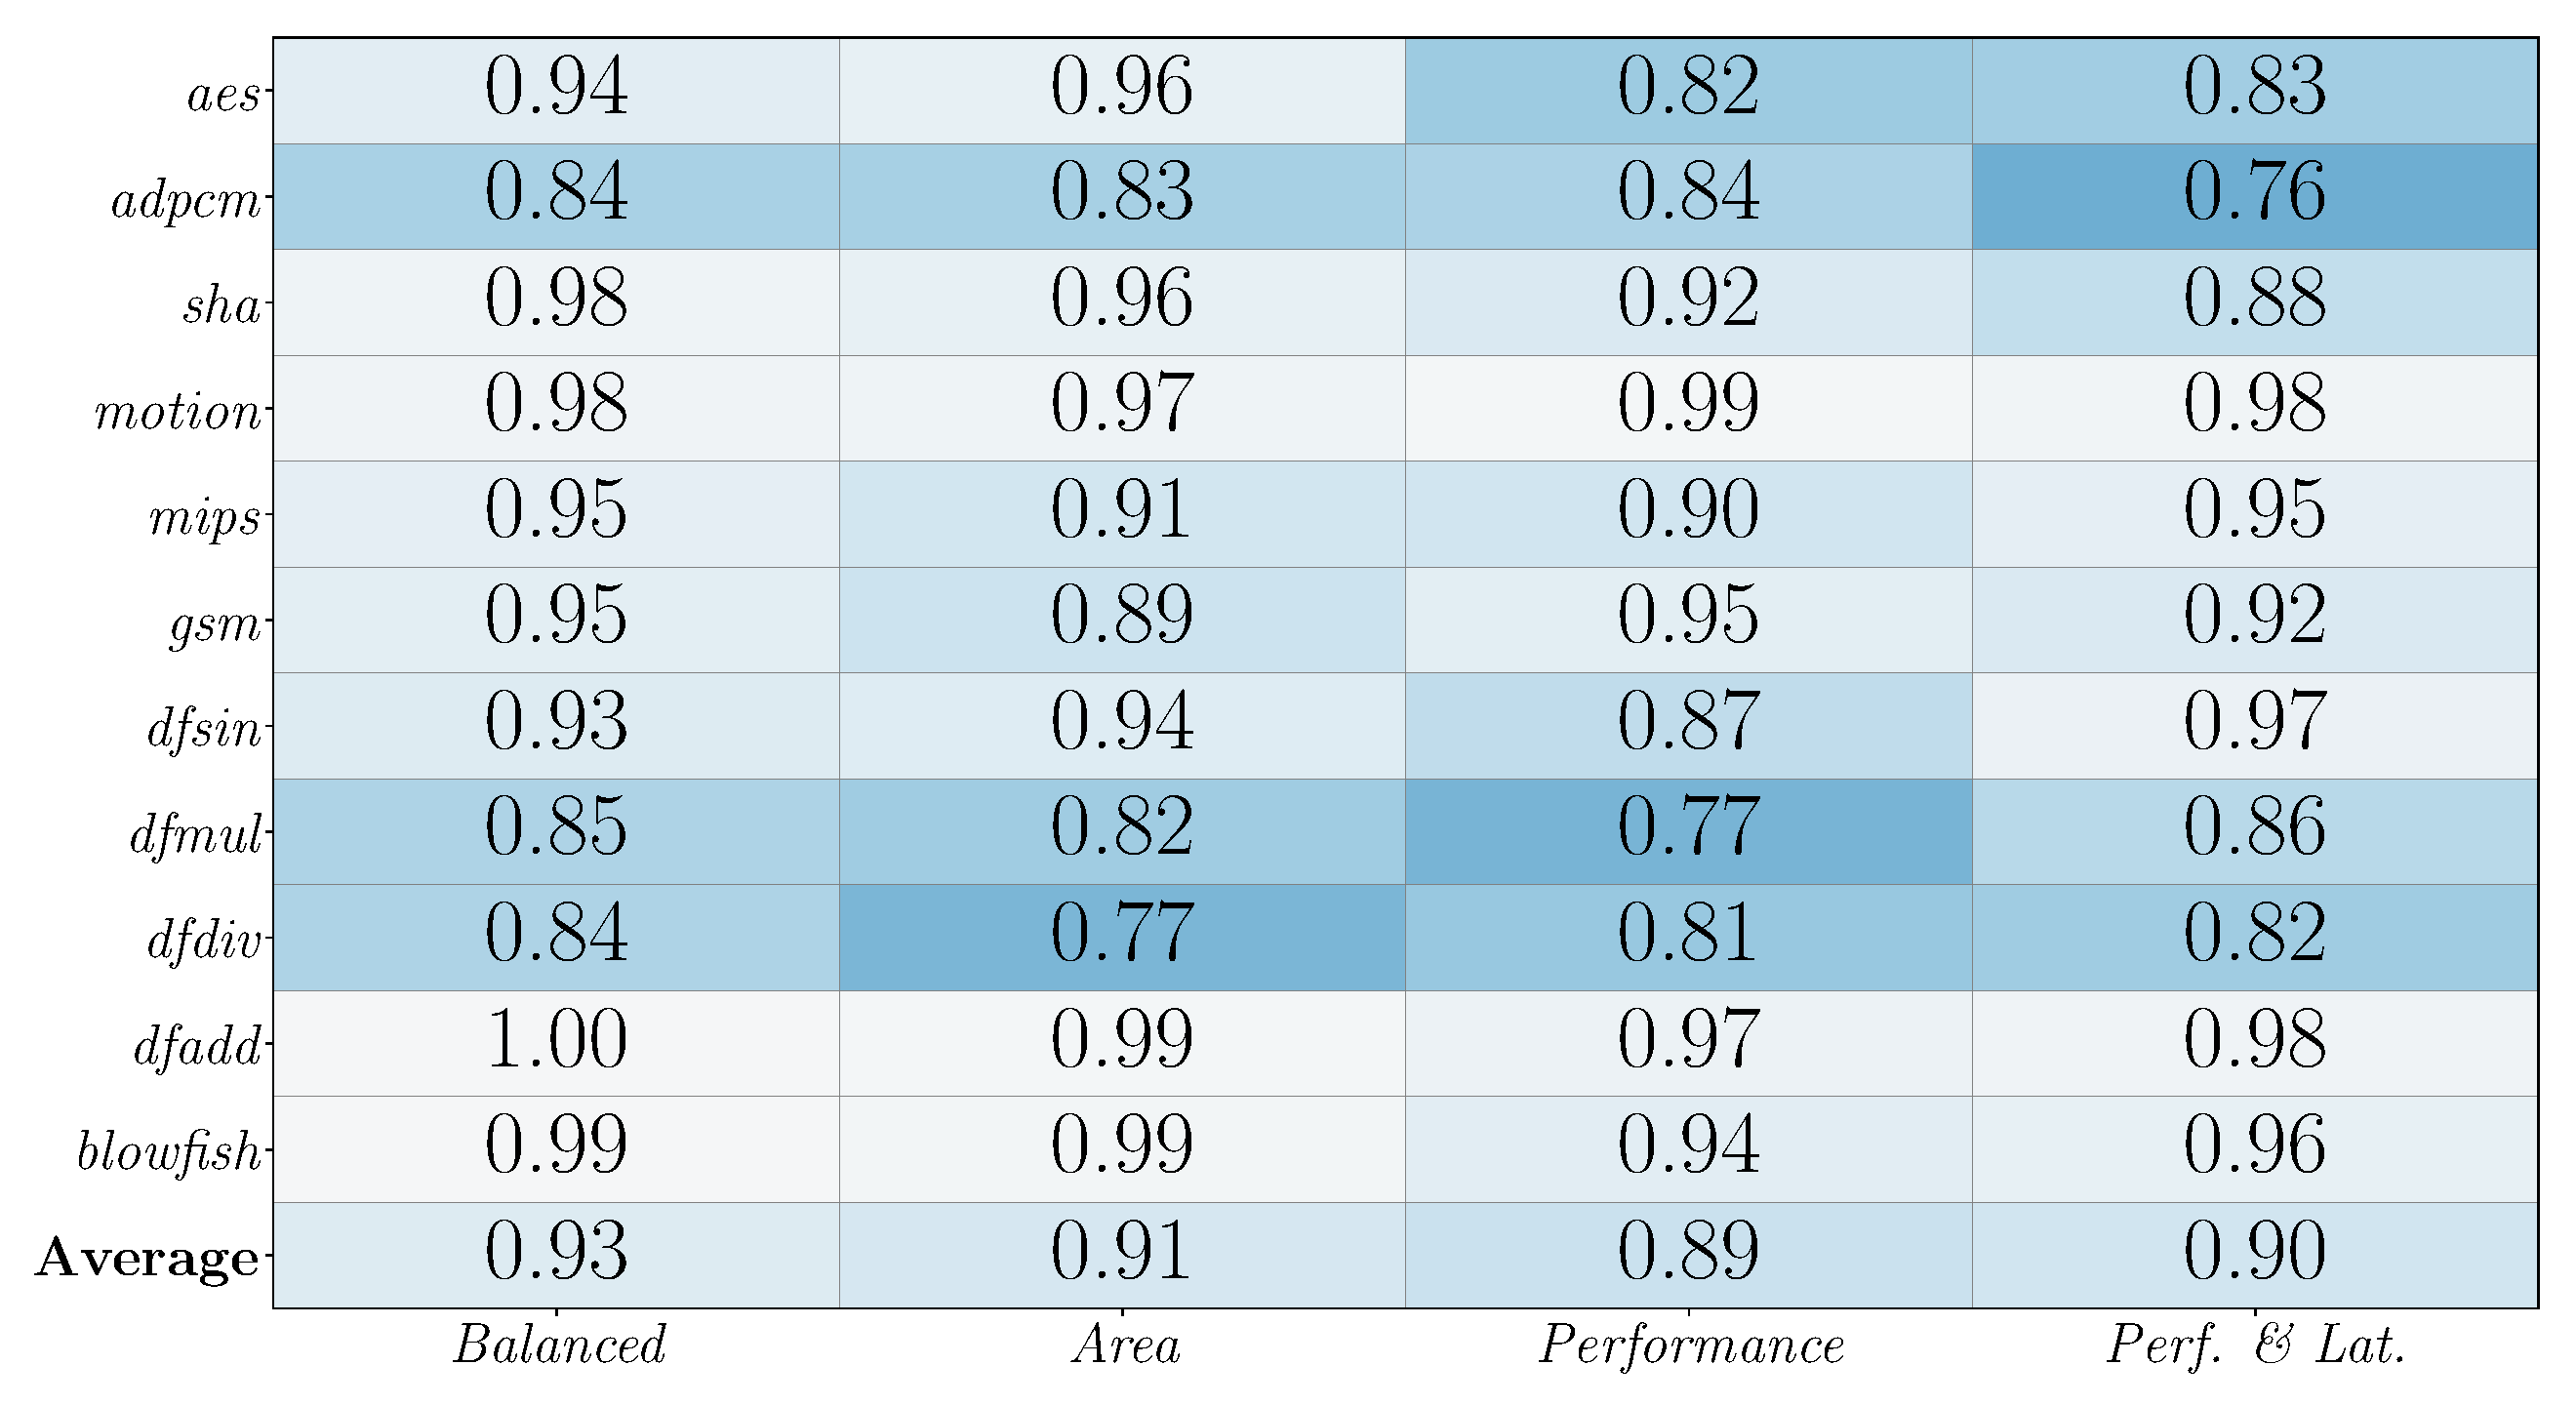
\includegraphics[width=0.5\columnwidth]{heatmap_wns_comparison}
    \caption{Relative improvement for \textbf{WNS} in all scenarios}
    \label{fig:wns-comp}
\end{figure}

\subsection{Summary}
\label{sec:FPGAconcl}

The results of this experiment show that it is always valuable to have a
sensible starting position for an autotuner. This becomes more relevant as the
size of the search space and the number of targeted metrics increase.  The
flexibility of our virtualized approach is evidenced by the results for
different optimization scenarios.  Improvements in \textbf{WNS} increased when
higher weights were assigned to metrics that express a coherent objective such
as area, performance and latency.  The improvements of metrics related to those
objectives also increased.

Future work in this direction will study the impact of different starting points on the
final tuned values in each optimization scenario, for example we could start
tuning for \textit{Performance} at the best autotuned \textit{Area} value.  We
expected that starting positions tailored for each target application will
enable the autotuner to find better \textbf{WNS} values faster.  We will also
apply this autotuning methodology to HLS tools that enable a fast prediction of
metric values. These tools will enable the exploration of the trade-off between
prediction accuracy and the time to measure an HLS configuration.

\section{Autotuning and Distributed Computing}
\label{sec:autotuningCloud}

In this study we developed a new methodology and a protocol for the
distributed execution of autotuners using cloud computing resources.  The
methodology and protocol are implemented as extensions to the OpenTuner
framework distributing and parallelizing the exploration of optimization spaces
by combining results obtained from virtual machines.  A local machine (LM) runs
the main OpenTuner application. Several virtual machines (VMs) run measurement
modules and provide results when requested. This distributed approach performs
a more cost efficient exploration of the search space in comparison to the
sequential execution.

The interactions between the LM and VMs follow the
client-server model. The LM runs a measurement client that requests
results from various measurement servers running in VMs hosted at
a public cloud. The experiments in this study used the Google Compute Engine
(GCE).  We compare the performance of our methodology, implemented as an
OpenTuner extension, with the unmodified framework using two instances of the
Travelling Salesperson Problem.

In a progression of
papers~\cite{gupta2012exploring,gupta2014evaluating,gupta2013hpccloud}, Gupta
\emph{et al.} provide experimental evaluations of the application of cloud
computing to high performance computing, describing which kind of applications
has the greatest potential to benefit from cloud computing.  Their work
highlights small and medium scale projects as the main beneficiaries of cloud
computing resources. This is a strong motivation for performing autotuning
runs using those resources.

This section is organized as follows.
Section~\ref{sec:ext} presents the proposed methodology, the architecture of
the measurement driver extension, the GCE interface and the application
protocol.
Section~\ref{sec:norm} discusses the result normalization strategies.
Section~\ref{sec:exp} describes the experiments performed and the
application used in the benchmark.
Section~\ref{sec:results} discusses the results obtained.
Section~\ref{sec:cloud-conclusion} concludes.

\subsection{Methodology and Protocol}
\label{sec:ext}

The methodology and protocol proposed in this study follow the client-server
model, distributing measurements of program configurations between a group of
VMs running \emph{MeasurementServer}s in the cloud. The servers wait for
measurement requests from a client, and maintain copies of the program to be
autotuned and the user-defined function that measures configurations.

An interface encapsulates the communication from the client enabling a
considerably lower implementation effort for the client.
Figure~\ref{fig:loc-comp} shows a rough estimate of the implementation effort
for the three components needed to implement our methodology and protocol.

The machine running the OpenTuner autotuner runs a \emph{MeasurementClient}, an
extension of the native \emph{MeasurementDriver}, that instead of compiling and
running result requests locally, uses an interface to route requests to VMs and
then saves the results to the local database.

\begin{figure}[htpb]
    \centering
    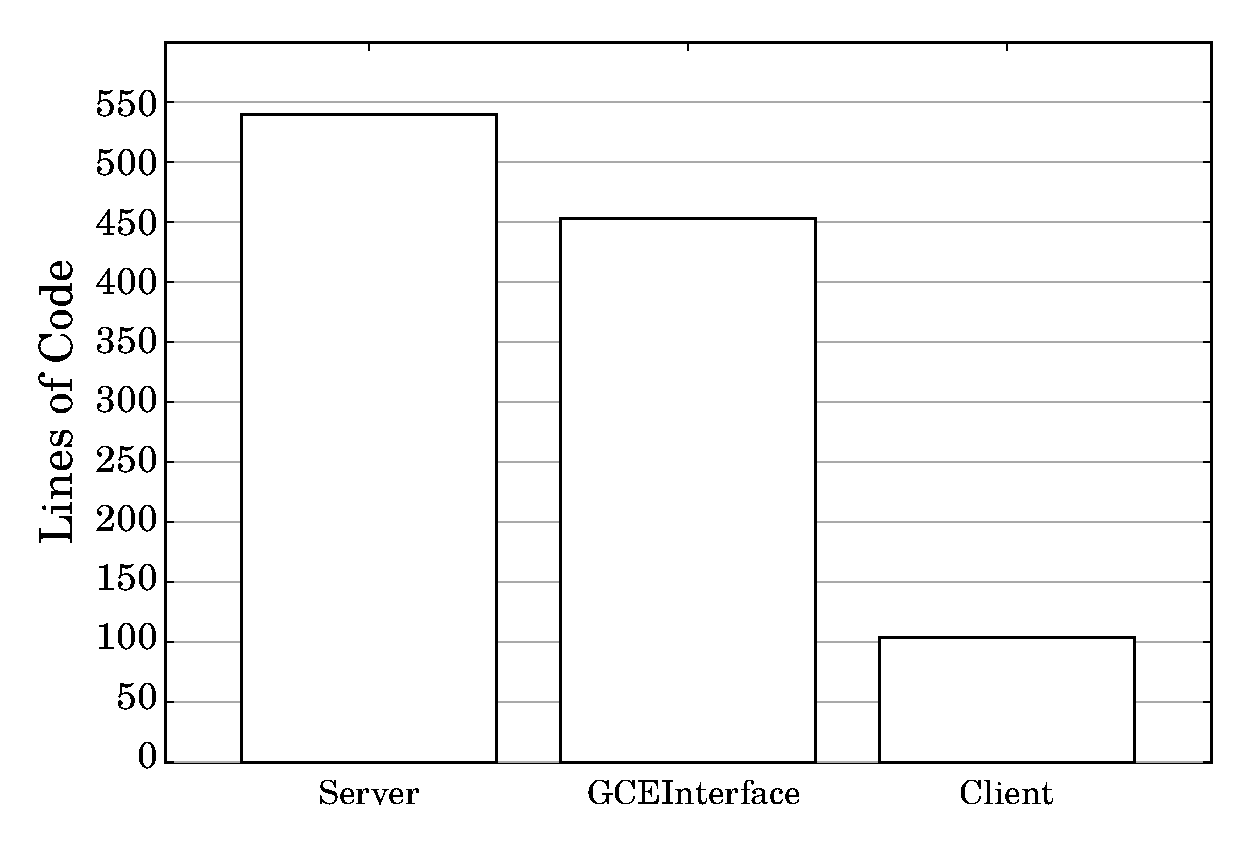
\includegraphics[scale=.35]{loc_comparison}
    \caption{An estimate of the implementation effort, measured in lines of
    code.}
    \label{fig:loc-comp}
\end{figure}

Figures~\ref{fig:high-level} and~\ref{fig:low-level} present an overview of the
architecture of the extension.  Figure~\ref{fig:high-level} presents the
architecture of an OpenTuner application running the measurement client and
communicating with the measurement servers.  Green boxes in the figure
represent OpenTuner modules that are not modified, and blue boxes represent new
or modified modules.

Figure~\ref{fig:low-level} shows, on a lower level of abstraction, the
interactions between the measurement client and servers. The client requests
results from the server through a wrapper of the GCE Python API.  The GCE
interface also encapsulates the application protocol used in the client-server
communication.

The remaining of this section describes the extension implementation in further
detail, the GCE interface and the application protocol.

\begin{figure}[htpb]
    \centering
    \begin{minipage}{.45\textwidth}
        \centering
        \includegraphics[scale=.64]{high-level-implementation}
        \caption{A high-level view of the architecture.}
        \label{fig:high-level}
    \end{minipage}%
    \hfill
    \begin{minipage}{.45\textwidth}
        \centering
        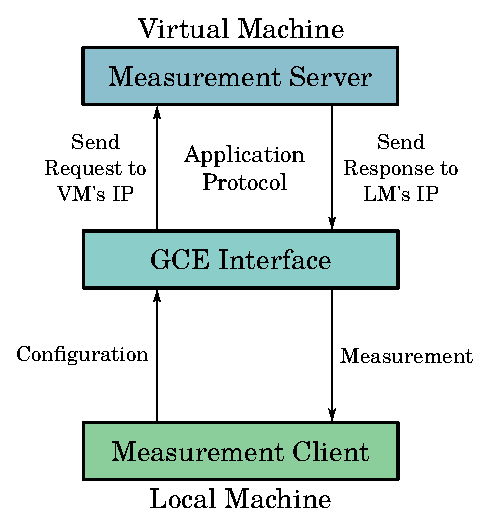
\includegraphics[scale=.64]{low-level-implementation}
        \caption{A lower-level view of the architecture.}
        \label{fig:low-level}
    \end{minipage}%
    \label{fig:archs}
\end{figure}

\subsubsection{Measurement Server and Client}
\label{sec:server-client}

OpenTuner controls the execution flow of an application with the
\texttt{\footnotesize main} function of the \emph{TuningRunMain} class. This
function initializes the database and the search and measurement modules. It
then calls the \texttt{\footnotesize main} function of the search driver, which
runs the main loop of the application.  The search driver generates
configurations to be tested and saves them to the database. It then calls the
\texttt{\footnotesize process\_all} function of the measurement driver and
blocks until the function returns.

The \texttt{\footnotesize process\_all} function calls the
\texttt{\footnotesize run\_desired\_results} function, which is able to run
compilations in parallel but only sequential measurements.  The modified
\emph{MeasurementDriver} initializes the GCE interface during its own
initialization. During execution the overridden \texttt{\footnotesize
process\_all} and \texttt{\footnotesize run\_desired\_results} functions route
the result requests to the VMs using the \emph{GCEInterface}.

An instance of the \emph{MeasurementServer} runs in every VM. The server waits
for TCP connections from a single client.

\subsubsection{GCE Interface}
\label{sec:gce}

The interactions between the local \emph{MeasurementClient} and the VMs'
\emph{MeasurementServer}s are mediated by the \emph{GCEInterface}, a wrapper of
the GCE Python API.  The interface starts and configures VMs storing each
measurement server's IP.

The interface enables the \emph{MeasurementClient} to request results from the
servers without knowledge of the application protocol. Running our
client-server methodology in another cloud environment would require a new
interface that manages VMs in this environment, but no modifications to the
server or client would be needed.

\subsubsection{Application Protocol}
\label{sec:app}

This section describes the text-based application protocol used in the
client-server communications mediated by the \emph{GCEInterface}. The user's
OpenTuner application must be a git project available via
\texttt{\footnotesize{HTTP}}. The application will be cloned to the VM by the server using the \texttt{\footnotesize CLONE} message.  The
application's \texttt{\footnotesize run} method will be used to obtain
autotuning results requested by the client.

\paragraph{Messages}
\begin{table}[htpb]
    \centering
    \scriptsize
    \begin{tabular}{@{}p{1.95cm}p{3cm}p{4.5cm}@{}}
        \toprule
        {\bf Command} & {\bf Function} & {\bf Message} \\ \midrule
        {\scriptsize \bf START} &
        {\scriptsize Sets the server's status to AVAILABLE} &
        {\scriptsize \tt \lq{}START\rq{}} \\ \midrule
        {\scriptsize \bf STOP} &
        {\scriptsize Sets the server's status to STOPPED} &
        {\scriptsize \tt \lq{}STOP\rq{}} \\ \midrule
        {\scriptsize \bf STATUS} &
        {\scriptsize Requests the server current status} &
        {\scriptsize \tt \lq{}STATUS\rq{}} \\ \midrule
        {\scriptsize \bf DISCONNECT} &
        {\scriptsize Disconnects from the server} &
        {\scriptsize \tt \lq{}DISCONNECT\rq{}} \\ \midrule
        {\scriptsize \bf SHUTDOWN} &
        {\scriptsize Disconnects and shuts the server down} &
        {\scriptsize \tt \lq{}SHUTDOWN\rq{}} \\ \midrule
        {\scriptsize \bf CLONE} &
        {\scriptsize Clones a git repository to the virtual machine} &
        {\scriptsize \tt \lq{}CLONE REPO\_URL DIST\_DIR\rq{}} \\ \midrule
        {\scriptsize \bf LOAD} &
        {\scriptsize Imports the user's MeasurementInterface into the server} &
        {\scriptsize \tt \lq{}LOAD TUNER\_PATH INTERFACE\_NAME\rq{}} \\ \midrule
        {\scriptsize \bf MEASURE} &
        {\scriptsize Computes the measurement for a given configuration} &
        {\scriptsize \tt \lq{}MEASURE CONFIG INPUT LIMIT\rq{}} \\ \midrule
        {\scriptsize \bf GET} &
        {\scriptsize Requests a configuration's result} &
        {\scriptsize \tt \lq{}GET RESULT\_ID\rq{}} \\ \bottomrule
    \end{tabular}
    \caption{Server messages.}
    \label{tab:protocol-messages}
\end{table}

Table~\ref{tab:protocol-messages} shows all the messages in the protocol, a
brief description of their meaning and their string format. The client must
send a \texttt{\footnotesize MEASURE} message for each configuration that is
measured. The server returns a unique ID that is used to retrieve the results
when they are ready. This is done by sending a \texttt{\footnotesize GET}
message.

\paragraph{Server Responses}

The server responds to each request with a message template and trailing,
message-specific parameters. Responses always start with the correspondent
command name and end with a newline character.  Each response contains the
current server status (\texttt{\footnotesize SERVER\_STATUS}) and error code of
the command (\texttt{\footnotesize ERROR\_STATUS}).  The optional argument list
(\texttt{\footnotesize [ARGS..]}) contains the measurement result, for example,
in the case of a successful \texttt{\footnotesize GET} response.
Figure~\ref{fig:response-template} shows the format of a server response.

\begin{figure}[htpb]
    \centering
    \footnotesize
    \begin{tabular}{@{}c@{}}
        \toprule
        {\tt \lq{}COMMAND ERROR\_STATUS SERVER\_STATUS [ARGS..] [MESSAGE]\rq{}} \\ \bottomrule
    \end{tabular}
    \caption{The format of a server response.}
    \label{fig:response-template}
\end{figure}

All the code implemented for the proposed methodology and protocol is publicly
available at \path{github.com/phrb/measurement-server},
\path{github.com/phrb/gce_interface} and
\path{github.com/phrb/measurement_client} under the GNU General Public License.

\subsection{Result Normalization}
\label{sec:norm}

The VM instances available in public cloud computing services vary in multiple
aspects, such as available memory, number of processing cores and disk size.
When autotuning a program for a certain target machine, using instances hosted
at a public cloud, it is typical that the target architecture will differ from
the VMs'. Depending on the configuration of the cloud application the instances
could also have different architectures.

To effectively leverage cloud computing resources for autotuning, a
normalization technique must be devised that enables the results found in the
VMs to be valid for the target machine.  We present four approaches to this
problem. The best approach for each problem domain must be experimentally
determined, and could be a combination of the approaches described here.

\paragraph{Autotune Performance Models}
Another autotuner could be implemented to optimize parameters of a simple
performance model, that would associate a configuration's measurement and the
VM that produced it with a conversion function that transposes
performance results to the target architecture.

\paragraph{Ensembles of Virtual Machines}
The cloud application could be composed of VMs with different architectures.
The final performance measurement for a configuration would be built from some
combination of the results obtained in these different VMs.

\paragraph{Architecture Simulators}
The target machine could be modeled by an architecture simulator such as
\emph{zsim}~\cite{sanchez2013zsim}, a simulator for multi-core architectures.
Using a simulator would solve the normalization problem but introduce other
problems, such as the simulator's accuracy and performance.

\paragraph{Autotune in the Cloud}
Finally, the normalization problem could be sidestepped, at least in initial
stages of research, by running the servers and clients in the cloud using the
same kind of VM.

\subsection{Experiments}
\label{sec:exp}

This section describes the Travelling Salesperson Problem (TSP), the Google
Compute Engine's virtual machines and project settings used to evaluate the
efficacy of the proposed methodology and protocol.  The performances of
the autotuner for the TSP were measured in 8 different
experimental settings. Each tuning run lasted 15 minutes, used 2 or 4
virtual machines, and was repeated 4 times.  We also varied the number of
result requests that each virtual machine in a tuning run processed, namely 1,
4, 8 or 16 requests per machine.
The LM used had an 8-core Intel Xeon E3 and 32GB of RAM.

\subsubsection{Using the Google Compute Engine}

All virtual machines used in the experiments had a single vCPU and 3.75GB of
RAM (Google Compute Engine machine type \texttt{\footnotesize n1-standard-1}).
All experiments were performed with machines from the \texttt{\footnotesize
us-central1-f} zone. We built a virtual machine image with the latest stable
Debian distribution and all dependencies installed, speeding up the virtual
machines' initialization time.

\subsubsection{Travelling Salesperson Problem}

The instances of the TSP used in the experiments in this study were obtained
from TSPLIB~\cite{reinelt1991tsplib}.  A TSP solver was implemented as an
OpenTuner application. The search space was defined by all the possible
permutations, or tours, of cities where the first and last cities are the same.
We used two instances, of size 532 and 85900.

\subsection{Results}
\label{sec:results}

This section presents the results for all tuning runs for the TSP instances of
sizes 532 and 85900.  Figures~\ref{fig:85900boxplot} and~\ref{fig:532boxplot}
show the distributions of the costs of the best solutions found for the two
instances after 4 separate runs. It shows data for 2 and 4 VMs hosted in the
cloud and receiving different numbers of simultaneous result requests.  The
figures also show the distribution of the results obtained by running the
autotuner in the target machine with the unmodified OpenTuner.  The cost of the
solutions is measured as the weight of a tour in the graph defined by the
instances.

\begin{figure}[htpb]
    \centering
    \begin{minipage}{.48\textwidth}
        \centering
        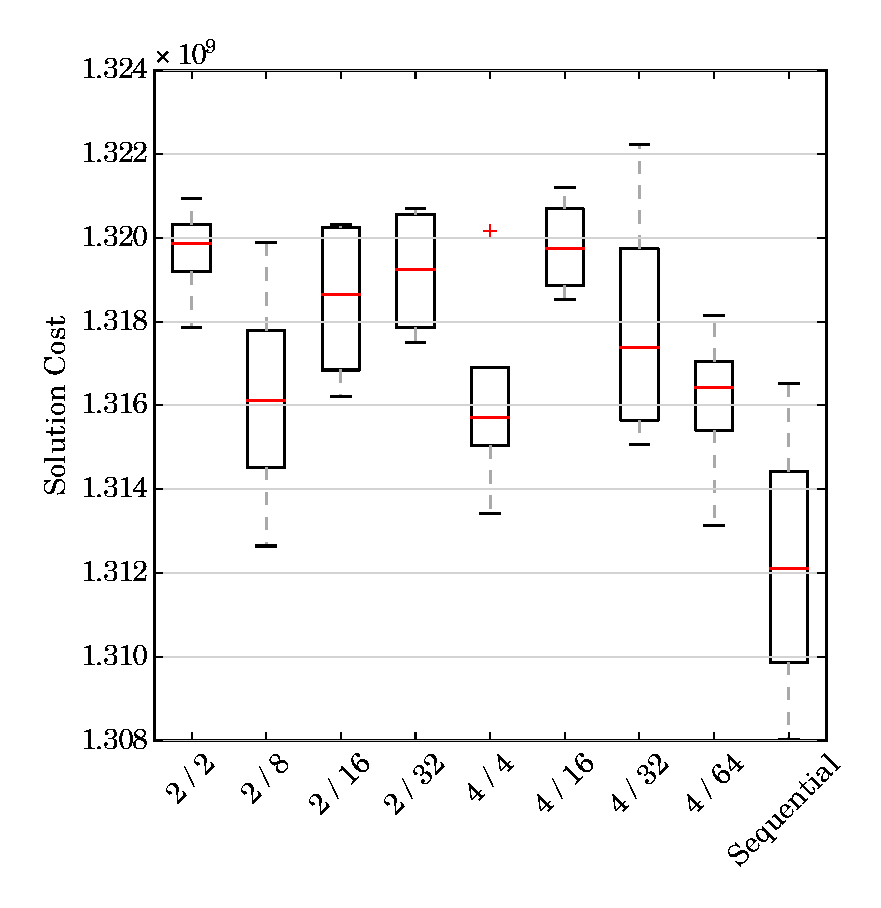
\includegraphics[scale=.48]{pla85900_15min_boxplot}
        \caption{Boxplots of 4 runs solving an instance of size 85900 with
                 different numbers of VMs and requests per VM.}
        \label{fig:85900boxplot}
    \end{minipage}%
    \hfill
    \begin{minipage}{.48\textwidth}
        \centering
        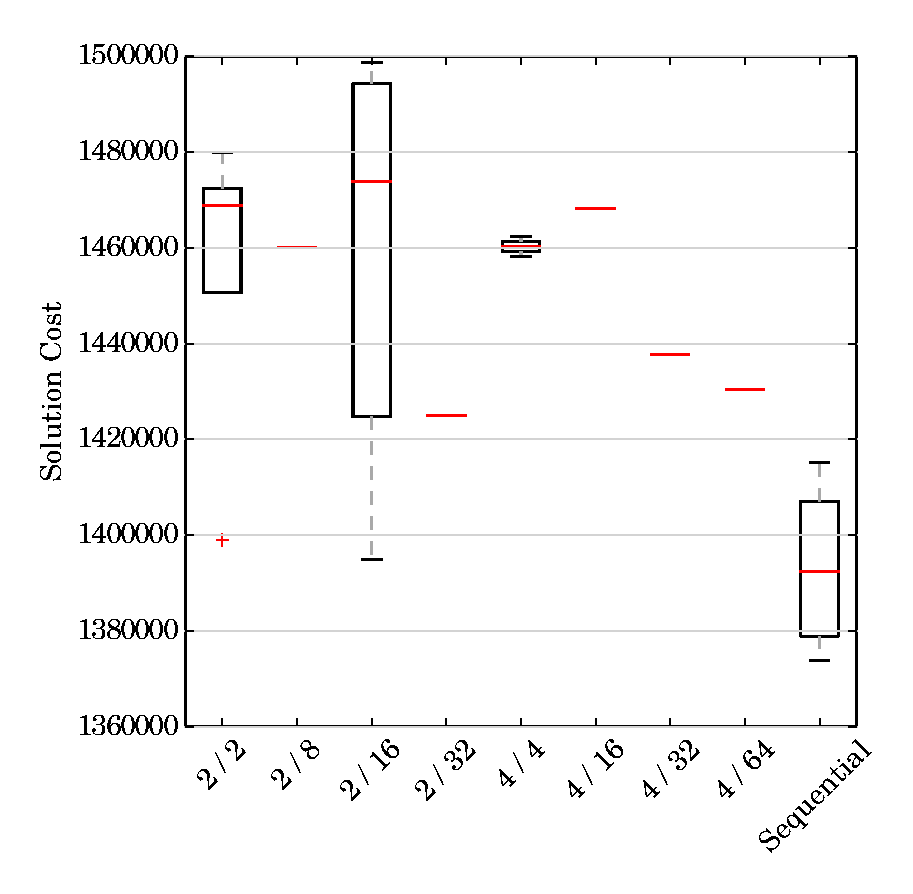
\includegraphics[scale=.48]{att532_15min_boxplot}
        \caption{Boxplots of 4 runs solving an instance of size 532 with
                 different numbers of VMs and requests per VM.}
        \label{fig:532boxplot}
    \end{minipage}%
    \label{fig:boxplots}
\end{figure}

Figures~\ref{fig:532tspi2} and~\ref{fig:532tspi4} show the best runs in the
instance of size 532 for the unmodified OpenTuner and for each VM
configuration.  Figures~\ref{fig:85900tspi2} and~\ref{fig:85900tspi4} show the
same measurements for the instance of size 85900.  The time overhead in
relation to the unmodified OpenTuner is clearly visible in
Figures~\ref{fig:532tspi2} to~\ref{fig:85900tspi4}, and is due to the
initialization of the cloud application.

\begin{figure}[htpb]
    \centering
    \begin{minipage}{.48\textwidth}
        \centering
        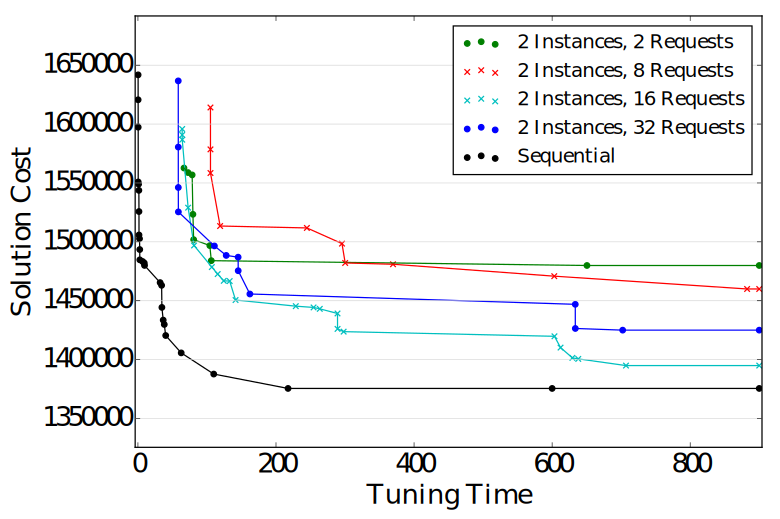
\includegraphics[scale=.43]{i2_p_n_comparison}
        \caption{Measurements using two VM instances, solving
                 a TSP instance of size 532.}
        \label{fig:532tspi2}
    \end{minipage}%
    \hfill
    \begin{minipage}{.48\textwidth}
        \centering
        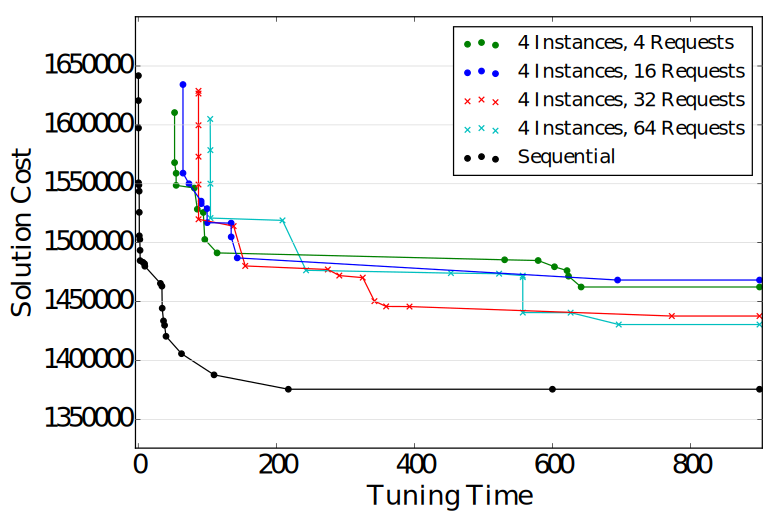
\includegraphics[scale=.43]{i4_p_n_comparison}
        \caption{Measurements using four VM instances,
                 solving a TSP instance of size 532.}
        \label{fig:532tspi4}
    \end{minipage}%
    \label{fig:532tsp}
\end{figure}

The tuning runs using our methodology and protocol depend on the initialization
of a cloud application, and start to produce results later in the tuning run.
Despite the graphs from figures~\ref{fig:532tspi2} to~\ref{fig:85900tspi4} show
that the solution costs of the results obtained with our methodology are worst
than the ones obtained with the unmodified OpenTuner, the cost of running the
same VM instance used in our experiments with the Google Compute Engine were as
low as
US\$0.038~\footnote{\path{cloud.google.com/compute/pricing#predefined_machine_types}
[Accessed on 23 December 2015]} per hour, per instance. The financial cost of
obtaining an autotuned solution of a given quality with our methodology is
therefore considerably lower than the financial cost of acquiring a machine
capable of finding the same solution. This is the main advantage of our
proposal.

\begin{figure}[htpb]
    \centering
    \begin{minipage}{.48\textwidth}
        \centering
        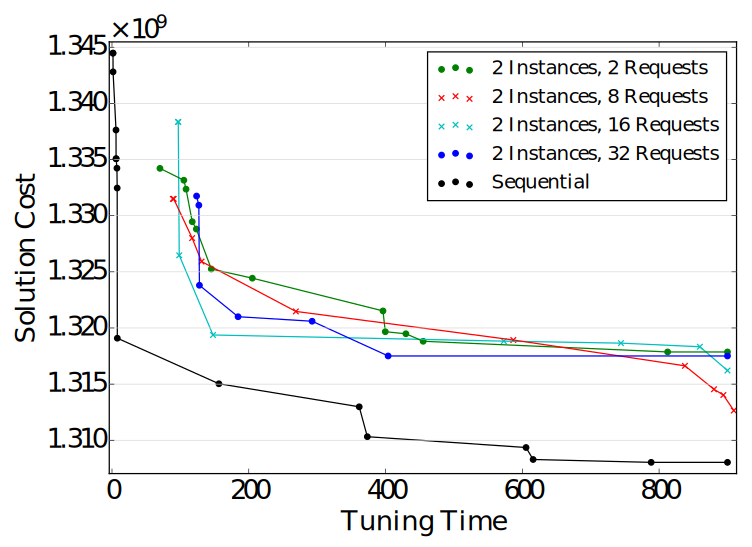
\includegraphics[scale=.43]{i2_p_n_comparison_85900}
        \caption{Measurements using two VM instances,
                 solving an instance of size 85900.}
        \label{fig:85900tspi2}
    \end{minipage}%
    \hfill
    \begin{minipage}{.48\textwidth}
        \centering
        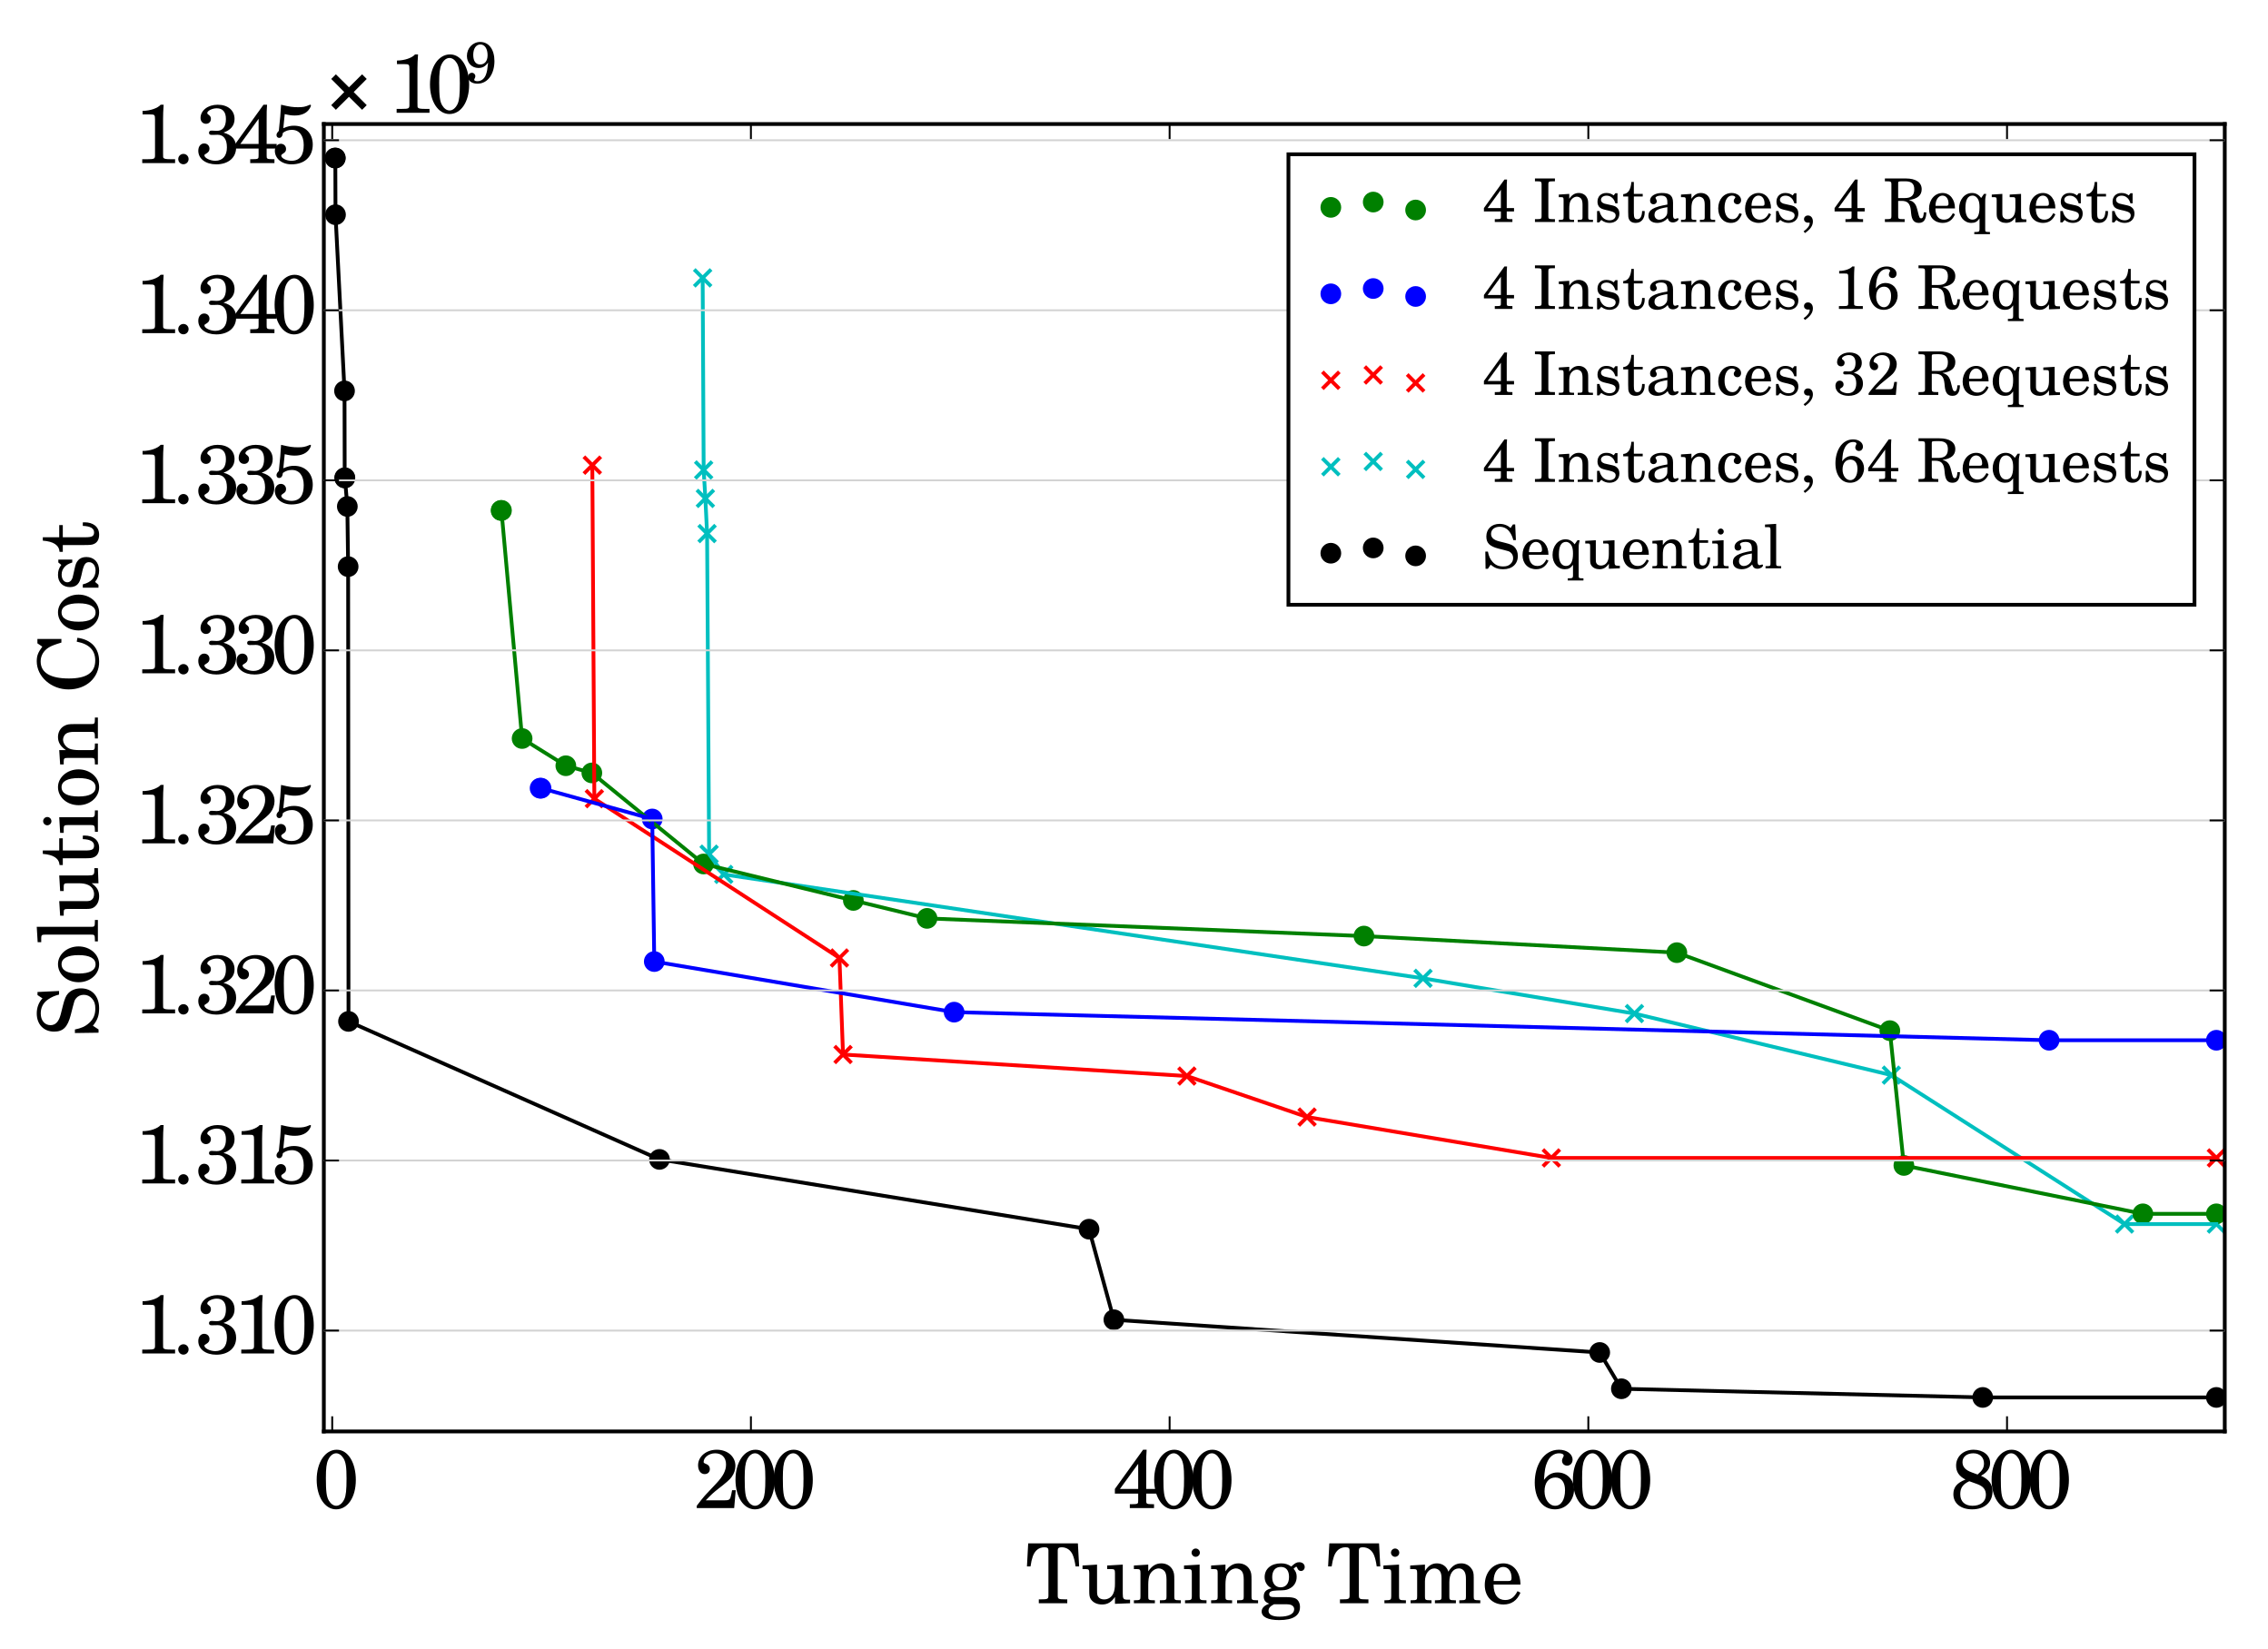
\includegraphics[scale=.43]{i4_p_n_comparison_85900}
        \caption{Measurements using four VM instances,
                 solving an instance of size 85900.}
        \label{fig:85900tspi4}
    \end{minipage}%
    \label{fig:85900tsp}
\end{figure}

\subsection{Parallel and Distributed Programming in OpenTuner}
\label{subsec:parallel}

\subsection{Summary and Future Work}
\label{sec:cloud-conclusion}

This study presented a methodology and an application protocol for distributing
autotuning measurements using cloud computing. We also presented an
implementation of the methodology and protocol, as an extension of the
OpenTuner autotuning framework.  We evaluated the performance and costs of our
methodology and protocol using instances of the Travelling Salesperson Problem
and the Google Compute Engine.  Our results show that the methodology reduces
the financial cost of finding a solution for the TSP.  We also proposed four
approaches to solve the result normalization problem which would enable
transposing the results obtained in VMs to a LM.

To the best of our knowledge, the methodology and protocol presented in this
study are the first to propose using cloud computing resources to reduce the
autotuning financial costs using the OpenTuner framework.

Future work will analyze the performance of our methodology and protocol in
different problem domains, determining the ones that benefit the most from this
approach. To effectively leverage cloud computing for autotuning it will be
necessary to better understand how VM initialization, communication and tuning
times impact performance. We would like to run more extensive experiments and
use different public clouds.

We will also study normalization techniques, composing benchmarks of problems
that expose architecture-dependant features to the autotuner and analyzing the
performance of our proposed techniques in those problems.

\section{Configuring Hardware and Software for the Dot Product Engine}
\label{sec:configDPE}

The Dot Product Engine (DPE)~\cite{hu2016dot} is a hardware accelerator for
matrix-vector multiplication using crossbar arrays to perform highly parallel
multiplications and additions through analog operations.  The concept is not
new~\cite{steinbuch1961lernmatrix,likharev2011crossnets}, with actual
implementations utilizing various technologies such as Flash, phase change
memories (PCM), and oxide-based memristors.  Circuit demonstrations have been
shown in stand alone platforms~\cite{prezioso2015training}, as well as part of
larger programmable analog computing systems~\cite{george2016programmable}.

A full architecture was recently proposed~\cite{shafiee2016isaac} that
integrates analog DPE components in a scalable, pipelined flow with digital
routing, buffers, and other components to flexibly support inference
computations for a broad range of Convolutional Neural Networks (CNN).  An
ISAAC chip is contains a number of tiles, composed of eDRAM buffers to store
input values, a number of in-situ multiply-accumulate (IMA) units, and output
registers to aggregate results.  All components are connected with a shared
bus.  Each IMA contains several crossbar arrays as well as shared ADCs.

A key performance aspect of the ISAAC architecture is the use of in-memory
processing, that is, memristor arrays not only store neural network weights,
but are also the location for computation. This reduction in data-fetching is
fundamental for performance improvement, but also imposes a strict data flow
that needs to be pipelined. Additionally, tiles can be partitioned between
different CNNs for a specific task.

Another parameter that impacts performance is the bit precision in matrix-vector
multiplication operations. Neural networks are highly tolerant of low
precision~\cite{courbariaux2014low, rastegari2016xnor, zhou2016dorefa}, which
reduces the load on ADCs. The precision needed to implement each neural network
layer is an important parameter to trade-off performance versus classification
accuracy.  Choosing the optimal operating point requires careful management.

Mapping neural network layers of various sizes to the appropriate physical
memristor crossbar arrays is a complex task.   Simply placing the neural
network layer in the largest possible array can lead to larger errors and
slower operating speeds.

The configuration optimization of data flow pipelines, tile partitioning,
operation bit precision and neural network mapping present opportunities to use
autotuners in the exploration of DPE hardware and software design spaces.  This
section presents our ongoing efforts on elaborating a search space for
autotuning that represents the hardware design space of the DPE.  We are
working with Hewlett-Packard Enterprise on this project.

\subsection{Background}

Many special-purpose accelerators have been proposed for neural network
acceleration~\cite{chen2014dadiannao,chi2016prime,shafiee2016isaac}, for which
dot-products are a fundamental operation.  Memristor-based DPEs have been shown
to be particularly promising~\cite{shafiee2016isaac} for computation patterns,
such as inference, where one of the operands is constant and frequently reused.
The DPE accelerates this operation by programming the constant operand into a
memristor crossbar and performing the computation in-situ with a streaming
input.

\subsection{Autotuning the Dot Product Engine}

Figure~\ref{fig:dpe-stack} shows the steps needed to generate a DPE
implementation from a hardware configuration or specification and to generate
application code using software parameters. These two steps present
autotuning opportunities for hardware and software parameters.

\begin{figure}[htpb]
    \centering
    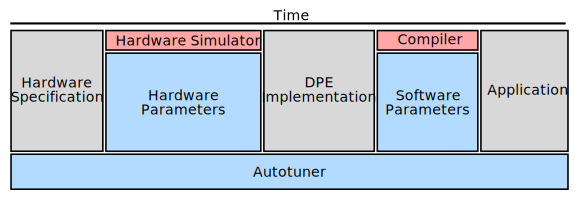
\includegraphics[width=.65\textwidth]{./images/dpe-stack}
    \caption{Steps from DPE hardware to software design and implementation}
    \label{fig:dpe-stack}
\end{figure}

We are using cycle-accurate simulators to obtain hardware metrics for different
DPE configurations, since the DPE architecture is still not defined.  The time
to obtain a working architecture simulation for a set of hardware parameters is
fast, since it consists of loading a configuration file.  We expect to use
simulators to explore the hardware design space before producing a prototype,
and autotuning will aid this exploration for different applications.
Figure~\ref{fig:overview-dpe-hard} shows the autotuner representation and time
scale for the current simulator-based workflow.

\begin{figure}[htpb]
    \centering
    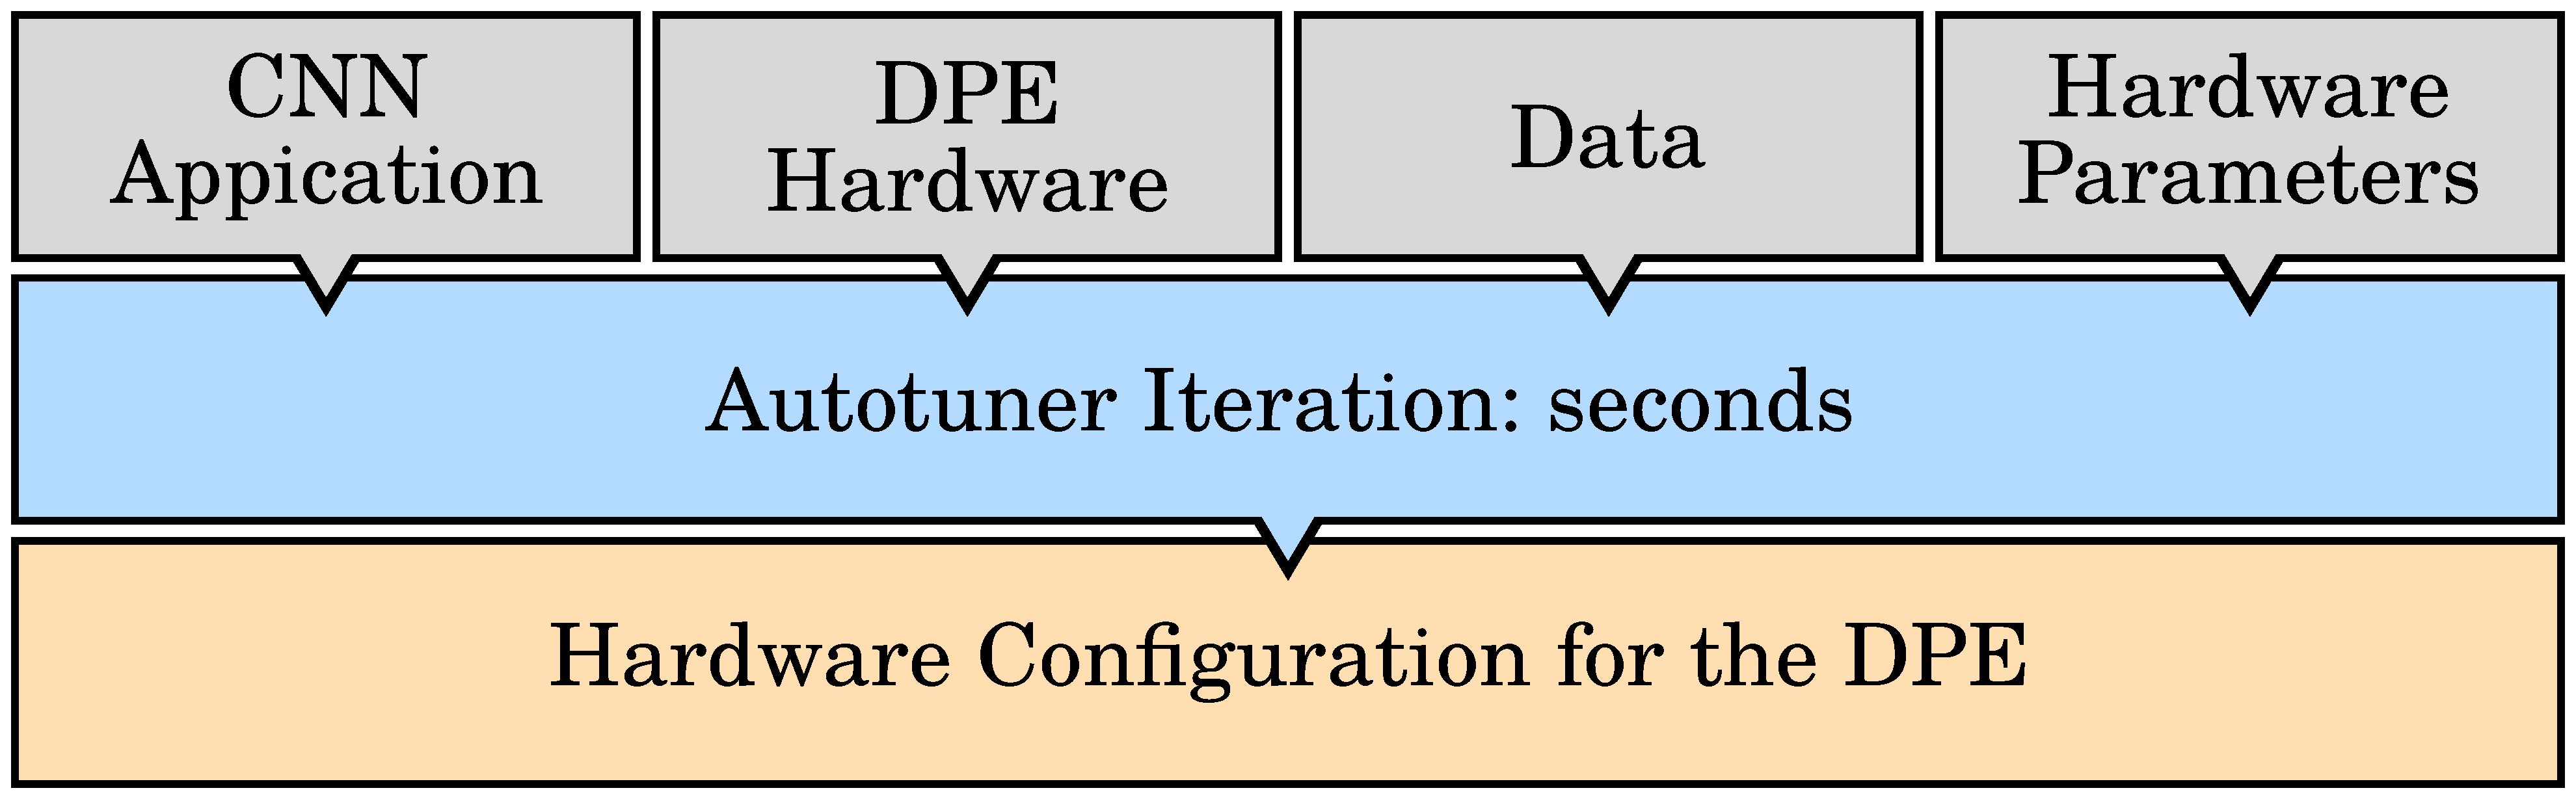
\includegraphics[width=.65\textwidth]{./images/overview_dpe_hard}
    \caption{Autotuner representation and time scale for hardware parameter
    autotuning}
    \label{fig:overview-dpe-hard}
\end{figure}

Figure~\ref{fig:overview-dpe-app} shows the autotuner representation and time
scale for software parameter autotuning. The simple applications that we are
using now have no parameters and take time in the order of seconds to complete.
The DPE code for these applications is also written by hand. We expect that the
code for future applications will be generated by a compiler, and compiling and
running time may vary.

\begin{figure}[htpb]
    \centering
    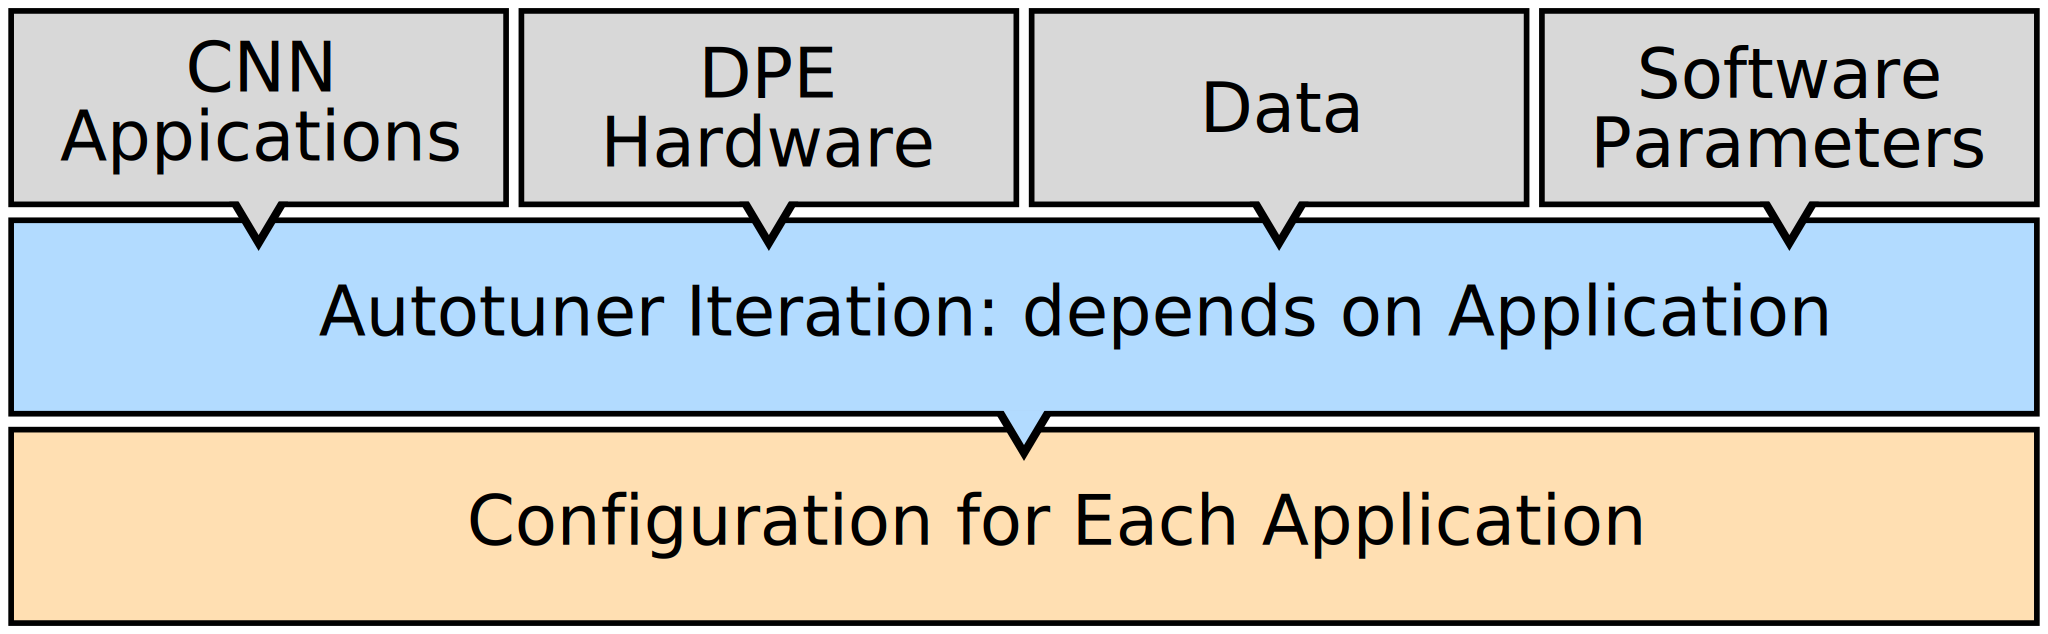
\includegraphics[width=.65\textwidth]{./images/overview_dpe_app}
    \caption{Autotuner representation and time scale for software parameter
    autotuning}
    \label{fig:overview-dpe-app}
\end{figure}

\subsection{Autotuner \& Search Space}
\label{sec:DPEautotuning}

This section presents the autotuner that we are implementing and the
preliminary search space we developed with DPE hardware design parameters.

\subsubsection{Autotuner}

\todo[inline,author=Pedro,color=cyan]{Describe autotuner implemented
in StochasticSearch and its current limitations}

\subsubsection{Search Space}

\todo[inline,author=Pedro,color=cyan]{Fix these tables}

Table \ref{tab:hard-soft-params} shows hardware and software parameters that
define a design and reconfiguration space for the DPE. The impact of these
parameters on several metrics can be measured using analytical models and
simulations.  Table \ref{tab:metrics-measurements} shows metrics and
measurement strategies that can be optimized for the DPE.

\begin{table}[htpb]
\centering
\begin{tabular}{@{}p{0.42\columnwidth}p{0.42\columnwidth}@{}}
\toprule
\textbf{Hardware} & \textbf{Software} \\ \midrule
Routing tables, eDRAM buffer size; bit size in IMA, layer; bus width; crossbar \& IMA number in tiles & Memristor arrays, layers \& routing tables mapping  \\
\addlinespace
ADC hardware configuration and heterogeneous tile designs & ADC and tile usage \\ \bottomrule
\addlinespace
\end{tabular}
\caption{Tunable software and hardware DPE parameters
}
\label{tab:hard-soft-params}
\end{table}

\begin{table}[htpb]
\centering
\begin{tabular}{@{}p{0.46\columnwidth}p{0.46\columnwidth}@{}}
\toprule
\multicolumn{2}{c}{\textit{Tuning Metrics and Measurements}} \\
\multicolumn{1}{c}{\textit{Metrics}} & \multicolumn{1}{c}{\textit{Measurements}} \\ \midrule
Bandwidth, latency, execution time, router area, throughput & Modelled area and power overhead for components \\
\addlinespace
Computation, power, crossbar efficiency & Cycle accurate simulation for: tile communication; eDRAM access \\
\addlinespace
Usability, flexibility & Empirical, qualitative \\ \bottomrule
\addlinespace
\end{tabular}
\caption{Tuning metrics \& measurement strategies for DPE}
\label{tab:metrics-measurements}
\end{table}

\todo[inline,author=Pedro,color=cyan]{Add results if possible}

\subsection{Summary}
\label{subsec:DPEconcl}
\todo[inline,author=Pedro,color=cyan]{Discuss that the simulator may produce
results very fast. Aayush mentioned that it takes around 2 seconds to simulate
the architecture with pre-generated assembly. It is still unclear for this case.}

\chapter[NODAL: an Open Distributed Autotuning Library]{NODAL: \\ an Open Distributed Autotuning Library}
\label{chap:julia}

This chapter presents NODAL, a domain-agnostic autotuning library written in
the Julia language, and
available~\footnote{\url{https://github.com/phrb/NODAL.jl} [Accessed in
17/10/2017]} under the MIT license.  NODAL has had continuous integration from
the start of the project, has 96\% of the relevant lines covered by unit tests
and an online documentation. NODAL's architecture and approach to
domain-agnostic autotuning is inspired by the OpenTuner
framework~\cite{ansel2014opentuner}. Autotuners using NODAL must define a
search space using the library's parameter types, and a cost function that
generates a program configuration and measures a performance metric.

The main contribution of NODAL is providing the capability of implementing
parallel and distributed search and measurement in autotuners for different
problem domains. NODAL's language selection, software architecture, and
execution flow were intended to solve the problems identified in the OpenTuner
framework, presented in section~\ref{sec:opentuner-parallel}.

NODAL is implemented in Julia, a high-level and high-performance language.
Julia programs are not limited by a Global Interpreter Lock, and are able to
leverage multi-core architectures and distributed computing resources.
Section~\ref{sec:julia} describes the Julia language and its parallel and
distributed programming model.

The search and measurement execution flows in NODAL are not centrally managed.
Each technique is able to request measurements and update its algorithm
independently. Multiple techniques can run in parallel in the same machine, or
distributed in multiple machines.  Techniques do not share global results and
can explore different regions of the search space.
Section~\ref{sec:nodal-arch} presents the current NODAL architecture, a
simplified call graph, and the improvements we have planned.
Section~\ref{sec:nodal-components} presents a more detailed view of each search
and measurement component.  Section~\ref{sec:nodal-examples} presents two
autotuners implemented using NODAL.

\section{The Julia Language}
\label{sec:julia}

Julia~\cite{bezanson2012julia,bezanson2014julia} is a dynamic programming
language, providing a high-level syntax and programming model.  Despite that,
Julia has performance comparable to widely used statically typed, low-level
languages. The time benchmarks~\footnote{Obtained from
\url{https://julialang.org/benchmarks/} [Accessed in 17/10/2017]} shown in
Figure~\ref{fig:julia_benchmarks} compare Julia's performance with other
high-level dynamic programming languages, using the performance in the C
language as a baseline.

\begin{figure}[htpb]
    \centering
    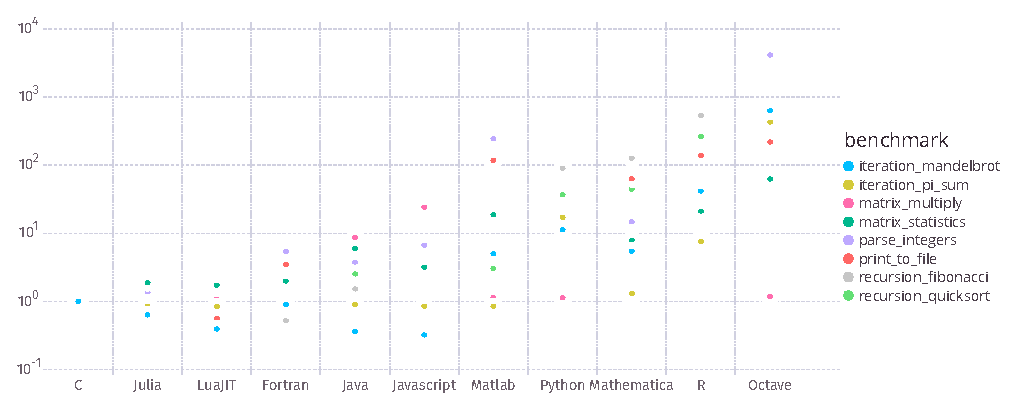
\includegraphics[width=.95\textwidth]{julia_benchmarks}
    \caption{Time benchmarks, relative to C, for various high-level languages}
    \label{fig:julia_benchmarks}
\end{figure}

The Julia developer community~\footnote{\url{https://github.com/JuliaLang/julia} [Accessed in
17/10/2017]} is very active, both in improving the standard library
and in developing separate packages, with over 1500 packages registered
in the language's official
repositories~\footnote{\url{https://pkg.julialang.org/} [Accessed in
17/10/2017]}, including NODAL.

Julia's high-performance, for a dynamic programming language, is attributed to
its type-inferred, Just-In-Time (JIT) compilation. Although a Julia program
can be written without type specifications, annotating variables with static
types is essential for performance.

\subsection{Parallel and Distributed Programming}
\label{sec:parallel-julia}

Julia's parallel and distributed programming model is based on message-passing
between processes. Each process has its own ID integer, and can run in a
separate processor core or machine. A Julia program does not manage multiple
processes, and is instead able to communicate using remote calls and
references, and data passed through channels.

Processes are launched and managed by cluster managers, which provide data
transport via TCP/IP in the built-in implementation. Cluster managers are also
able to manage the topology of the process network. NODAL currently uses the
built-in cluster manager, but studying the impact of different process
topologies might provide insight into improving NODAL's performance in
different distributed computing settings.

\subsubsection{Remote Calls \& References}

In Julia, a \textit{remote call} is a function call that is computed in a
different process. Remote calls can be made with the \texttt{remotecall}
function, or with macros from the \texttt{@spawn} family. The
\texttt{remotecall} function receives a regular function \texttt{f}, a process
ID, and the arguments to be passed to \texttt{f}. The \texttt{@spawn} macro
receives an expression, which can be a regular function call or any valid Julia
expression, and launches it in the next available Julia process.

Remote calls return immediately after launching the computation. The
results can be obtained using the \textit{remote reference} returned
by remote calls. Remote references are objects that reference data
stored in other processes, and can be of type \texttt{Future} or
\texttt{RemoteChannel}.

Figure~\ref{fig:remotecall_example} shows a code snippet that illustrates how
to use the \texttt{remotecall} function and the \texttt{@spawnat} macro. The
\texttt{@spawnat} macro receives as argument the target process in which to
launch the computation, in addition to a Julia expression. The Julia
interpreter can be launched with the \texttt{-p} argument, which receives an
integer and launches the correspondent number of Julia processes.

The code snippet in Figure~\ref{fig:remotecall_example} shows a remote call to
the \texttt{rand} function, to be launched in the process with ID 2. The other
arguments specify the 2 by 2 matrix that \texttt{rand} will fill with random
numbers. After this remote call, the computation has been launched in a remote
process, and a \texttt{Future} is returned. The interpreter does not wait for
the computation to finish and waits for new input.

\begin{figure}[htpb]
    \begin{minipage}{\linewidth}
    \begin{lstlisting}[language=C, basicstyle=\ttfamily\scriptsize,
        numbers=left,
        frame=no, showspaces=false, showstringspaces=false,
        numberstyle=\scriptsize,
        xleftmargin=1.5cm,
        keywords={%
            @spawnat, remotecall, Nullable, Any,
            fetch, Future, Array, Float64, julia%
        },
        otherkeywords={::, \&, \*, +, -, /, [, ], >, <}
    ]
% ./julia -p 2

julia> r = remotecall(rand, 2, 2, 2)
Future(2, 1, 4, Nullable{Any}())

julia> s = @spawnat 2 1 .+ fetch(r)
Future(2, 1, 5, Nullable{Any}())

julia> fetch(s)
2x2 Array{Float64,2}:
 1.18526  1.50912
 1.16296  1.60607
    \end{lstlisting}
    \end{minipage}
    \caption{Using Julia's \texttt{remotecall} function and the \texttt{@spawnat} macro}
    \label{fig:remotecall_example}
\end{figure}

The call to the \texttt{@spawnat} macro in line 6 of
Figure~\ref{fig:remotecall_example} calls the \texttt{fetch} function. This
function receives a \texttt{Future} and blocks until the result is computed by
the remote process. The \texttt{.+} syntax represents an operation in an array.
In this case, the operation is summing 1 to every element of the matrix
returned by \texttt{fetch(r)}. The \texttt{@spawnat} macro also returns a
\texttt{Future}.  Finally, the call to \texttt{fetch} in line 9 of
Figure~\ref{fig:remotecall_example} gets the final value computed by the two
remote calls. The \texttt{remotecall\_fetch} function is a more efficient way
of launching a computation in a remote process and immediately asking for the
results, if there is no computation that can be performed while the process
waits.

A \texttt{Future} caches the remotely computed value after the first call,
and returns it without process communication in subsequent calls. A process
can only write once to a \texttt{Future}. If a more extended communication
is required, the programmer needs to use remote channels.

\subsubsection{Remote Channels}

Figure~\ref{fig:remotechannel_example} shows a more complex parallel and
distributed programming example using remote channels to manage a worker pool
that performs arbitrary jobs. Remote channels are created in a specific
process, but any process with a reference to a remote channel is able to write
values to it using the \texttt{put!} function, and to read values from it using
the \texttt{take!} function. In remote channels from the standard library,
\texttt{put!} blocks until there is space in the channel and \texttt{take!}
blocks until there is a data object in the channel that can be taken, and
removing it from the channel when the call completes.

\begin{figure}[htpb]
    \begin{minipage}{\linewidth}
    \begin{lstlisting}[language=C, basicstyle=\ttfamily\scriptsize,
        numbers=left,
        frame=no, showspaces=false, showstringspaces=false,
        numberstyle=\scriptsize,
        xleftmargin=1.5cm,
        keywords={%
            @spawnat, remotecall, Nullable, Any,
            fetch, Future, Array, Float64, julia,
            while, true, function, end, put!,
            take!, sleep, RemoteChannel, Channel,
            Int, Tuple, const, addprocs, @schedule,
            @everywhere, for, in, myid, @async,
            remote_do, workers%
        },
        otherkeywords={::, \&, \*, +, -, /, [, ], >, <, put!, take!}
    ]
julia> addprocs(4)

julia> const jobs = RemoteChannel(()->Channel{Int}(32))

julia> const results = RemoteChannel(()->Channel{Tuple}(32))

julia> @everywhere function do_work(jobs, results) # Defines method everywhere
       while true
           job_id = take!(jobs)
           exec_time = rand()
           sleep(exec_time) # Simulates time doing work
           put!(results, (job_id, exec_time, myid()))
       end
   end

julia> function make_jobs(n)
           for i in 1:n
               put!(jobs, i)
           end
       end

julia> n = 12

julia> @schedule make_jobs(n)

julia> for p in workers()
           @async remote_do(do_work, p, jobs, results)
       end

julia> while n > 0 # print out results
           job_id, exec_time, where = take!(results)
           n = n - 1
       end
    \end{lstlisting}
    %$
    \end{minipage}
    \caption{Using Julia's \texttt{RemoteChannel}}
    \label{fig:remotechannel_example}
\end{figure}

The snippet in Figure~\ref{fig:remotechannel_example} uses other macros and
functions. The \texttt{addprocs} function adds a specific number of processes
to the worker pool. The \texttt{@everywhere} macro is used to define data, or a
function, in all available Julia processes. The \texttt{@schedule} and
\texttt{@async} macros add asynchronous expressions to the Julia scheduler.
The \texttt{remote\_do} function launches a function in a given worker or
worker pool object.

NODAL uses remote calls and references to perform measurements, and remote
channels to manage the communication between search techniques and the user
program. The following section will describe NODAL's architecture and its
parallel and distributed implementation.

\section{Software Architecture}
\label{sec:nodal-arch}

Our main concern when developing NODAL was to ensure that search techniques
were independent from each other, making and managing their own requests for
measurements. To achieve this objective we developed a software architecture
that minimizes communication between processes and does not block on requests
to channels. NODAL uses a custom non-blocking remote channel, the
\texttt{ResultChannel}. Search techniques manage their own execution flow, and
write their results to remote channels. A central control process regularly
polls those remote channels for results.

\begin{figure}[htpb]
    \centering
    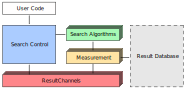
\includegraphics[width=.65\textwidth]{nodal_architecture}
    \caption{NODAL architecture, with a proposed database}
    \label{fig:nodal_architecture}
\end{figure}

Figure~\ref{fig:nodal_architecture} shows a high-level representation of
NODAL's architecture. User code that uses the library is responsible for
launching the main NODAL process, or \textit{tuning run}, and communicates with
it using remote channels. The NODAL main process is responsible for
initializing parallel and distributed search techniques using all processes
available. Each technique writes the best result it has found so far to its own
remote channel.  The main process has references for all technique remote
channels, and periodically polls them for results.  After technique
initialization there is no blocking communication between the main process and
search techniques, and no communication between search techniques.

Search techniques are responsible for generating candidate configurations for
evaluation and requesting their measurement. This is done using remote calls to
the user-defined cost function. After measurement is complete, search
techniques write the current result to their remote channel.  The non-blocking
remote channel implementation used in NODAL  is described in
section~\ref{sec:nodal-measurement}.

Figure~\ref{fig:nodal_architecture} shows a grayed out database component,
which is not yet implemented. This database will shorten the time to obtain
measurements of repeated configurations, and has the potential to be used to
train machine learning models or to give to the user knowledge about the search
space.

\subsection{Search and Measurement Call Graph}

A more detailed NODAL execution flow is presented in
Figure~\ref{fig:nodal_callgraph}. Each colored box represents a colored
component of Figure~\ref{fig:nodal_architecture}, and each smaller named box
represents a function of each component. When necessary, a number marks the
order in which functions are called.

The entry point of a NODAL application is the user code, which calls the
\texttt{optimize} function. This is the main NODAL process, and must be
launched using a remote call. The main process initializes remote search
techniques, using remote calls, by calling the
\texttt{initialize\_search\_tasks!} function. It is a non-enforced style of the
Julia language to append a ``\texttt{!}'' to functions that modify their
arguments. In this case, the modified argument is the list of remote channels
stored by the main process.  The initialization process is non-blocking, and it
returns after all techniques have been launched. The main process then enters a
loop, periodically checking for results from its remote channel references.
The \texttt{put!} and \texttt{take!} functions of \texttt{ResultChannel} are
non-blocking, so the main process always instantly gets a result from the
channel.

Initialized search techniques run their algorithms using search building
blocks, which are functions that perform some operation on the current
configuration of a search technique, measure it, and decide whether to accept
the new configuration. For example, the simulated annealing technique uses
the probabilistic improvement search building block.

\begin{figure}[htpb]
    \centering
    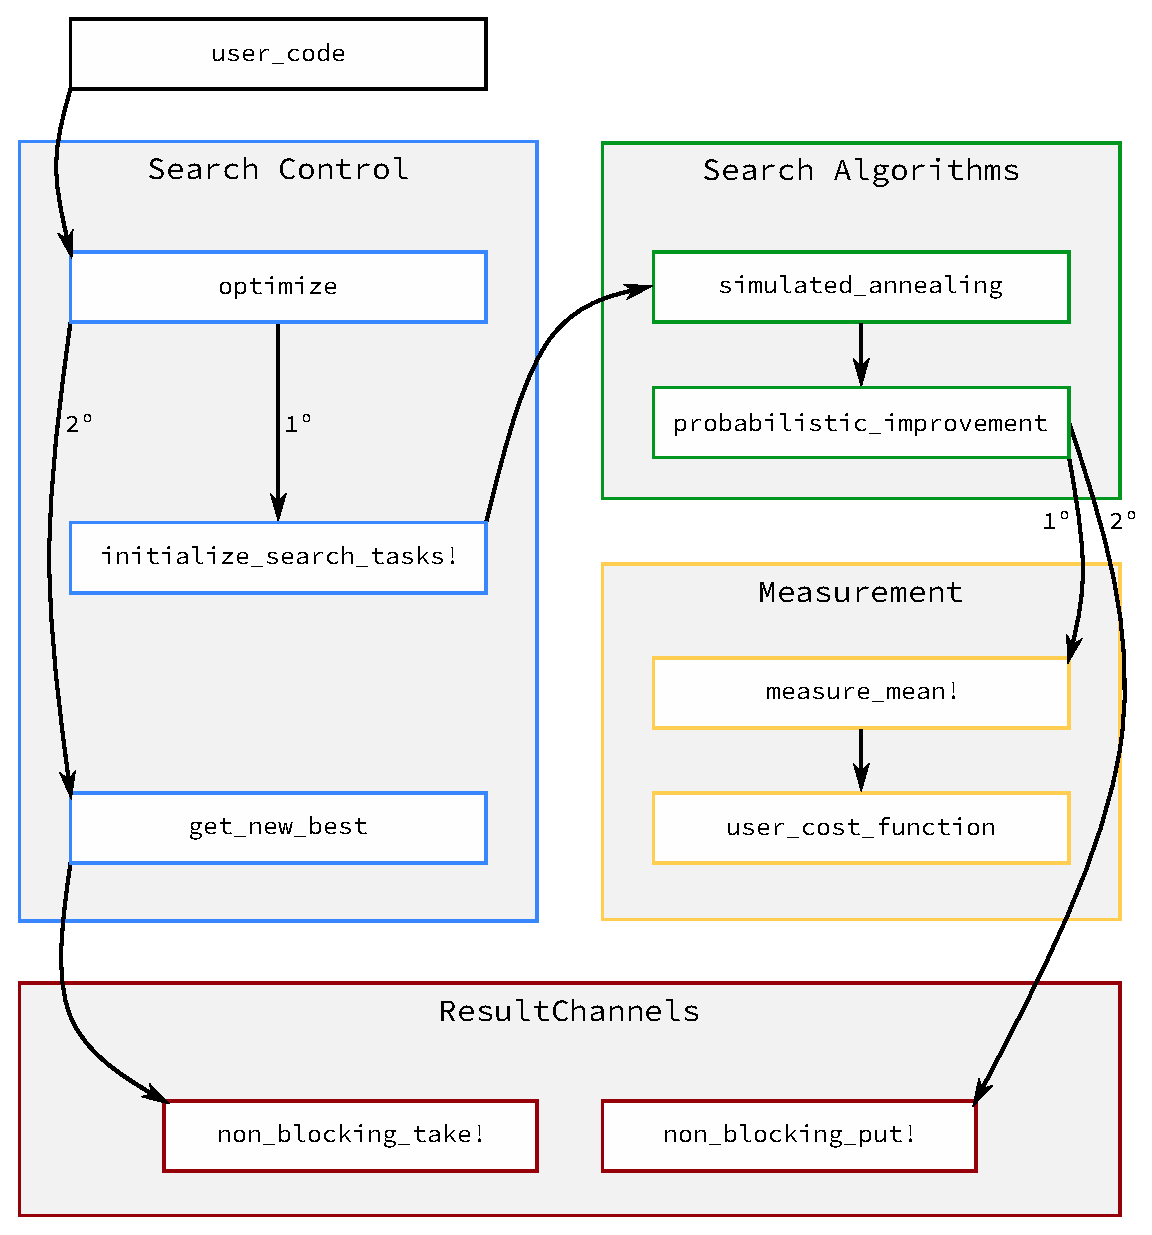
\includegraphics[width=.5\textwidth]{nodal_callgraph}
    \caption{NODAL search and measurement simplified call graph}
    \label{fig:nodal_callgraph}
\end{figure}

Search techniques request a measurement by performing remote calls to the
user-defined cost function. One way to do that is using the
\texttt{measure\_mean!} function, which perform multiple evaluations of a
function in parallel and returns the average of the measurements.  This is
useful for time measurements, for example, where fluctuations on the operating
system or system load can interfere with the results.

After a measurement is performed, a search technique can update its algorithm
and immediately request another measurement.  Search techniques do not share
their current best results with other techniques, but this was an
implementation choice and not an architecture limitation.  We intend to
implement a main process parameter that can be set by the user, and enables
global result sharing in cases where it may be beneficial. For example, the
user should be able to select which groups of techniques from the ensemble will
be allowed share their results.

\section{Search \& Measurement Components}
\label{sec:nodal-components}

This section presents in more detail the search and measurement components,
discussing available parameters, search techniques, and measurement methods.

\subsection{Search}

The search space of an autotuner implemented using NODAL is defined by a
\texttt{Configuration} object that contains a set of \texttt{Parameter}
objects. Parameters are changed by search algorithms by using operator
functions specific to each parameter type. Currently, the only operator
available in NODAL is the neighbor operator, that randomizes a parameter's
value inside a user-defined neighborhood. The ``radius'' of the neighborhood
can be changed on each call to the operator, enabling search techniques to
dynamically manipulate parameters.

\subsubsection{Parameters}

Parameters are used to define performance-impacting program variables and their
limits. They represent program configurations such as compiler flags,
enumerations of algorithms that solve a same problem, and any configurable
property of a program. Each parameter can have an initial value or left
uninitialized, in which case it will be randomized at the start of the search
process.  Table~\ref{tab:nodal-parameters} shows the parameters currently
implemented in NODAL and the planned additions.

\begin{table}[htpb]
\centering
\begin{tabular}{@{}p{.15\textwidth}p{.15\textwidth}@{}}
\toprule
\textit{Implemented} & \textit{Planned} \\ \midrule
Boolean & Logarithmic \\
Float & Exponential \\
Integer & Factorial \\
Enumeration & \\
Permutation & \\ \bottomrule
\end{tabular}
\caption{NODAL implemented and planned parameters}
\label{tab:nodal-parameters}
\end{table}

\subsubsection{Search Building Blocks}

Search building blocks are responsible for generating a new candidate
configuration and launching parallel measurements for it. Search techniques can
use one or more building blocks to implement their algorithms. Building blocks
enable users to implement parallel and distributed search techniques without
having to write parallel code in Julia or becoming familiar with NODAL
specifics. The implemented and planned building blocks at this stage of NODAL's
development comprise the necessary blocks for implementing the stochastic local
search algorithms presented by Hoos and Stützle~\cite{hoos2015stochastic}.
Other search building blocks may be necessary to implement future techniques.
Table~\ref{tab:nodal-blocks} shows the building blocks currently implemented in
NODAL and the planned additions.

\begin{table}[htpb]
\centering
\begin{tabular}{@{}p{.3\textwidth}p{.3\textwidth}@{}}
\toprule
\textit{Implemented} & \textit{Planned} \\ \midrule
First improvement & Best Improvement \\
Probabilistic Improvement & \\
Greedy Construction & \\
Random Walk & \\ \bottomrule
\end{tabular}
\caption{NODAL implemented and planned search building blocks}
\label{tab:nodal-blocks}
\end{table}

\subsubsection{Search Techniques}

The current available ensemble of search techniques in NODAL is composed of
stochastic local search techniques from the study by Hoos and
Stützle~\cite{hoos2015stochastic}.  Table~\ref{tab:nodal-techniques} present
the search techniques currently implemented in NODAL and the planned
additions.

\begin{table}[htpb]
\centering
\begin{tabular}{@{}p{.4\textwidth}p{.35\textwidth}@{}}
\toprule
\textit{Implemented} & \textit{Planned} \\ \midrule
Iterative First Improvement & Iterative Best Improvement \\
Iterative Greedy Construction & Randomized Best Improvement \\
Iterative Probabilistic Improvement & Randomized Best Improvement \\
Randomized First Improvement & Iterative Best Construction \\
Simulated Annealing & Dynamic Local Search \\
Iterated Local Search & Tabu Search \\
 & Ant Colony Optimization \\
 & Particle Swarm Optimization \\
 & Nelder-Mead \\
 & Genetic Algorithms \\ \bottomrule
\end{tabular}
\caption{NODAL implemented and planned search techniques}
\label{tab:nodal-techniques}
\end{table}

NODAL provides a simple way of creating new search techniques from building
blocks. Figure~\ref{fig:simulated_annealing} shows an implementation of the
simulated annealing search technique using the probabilistic improvement search
building block. This building block randomizes a configuration within a small
neighborhood, measures it, and accepts a worse configuration with a given
probability. This simulated annealing implementation uses a logarithmic
decreasing temperature as the probability for the probabilistic improvement
block.

Search technique functions must receive references to a \texttt{Run} object and
to a \texttt{RemoteChannel}.  The \texttt{Run} object contains the
configuration of the current tuning run, with data such as its duration,
configuration and cost function.

The search technique function must define an iteration function, which is
responsible for generating and measuring new configurations.  This function
must receive a tuning run object and return an object of type \texttt{Result}.
In NODAL, the \texttt{Result} object contains all information about a
configuration measurement, such as the iteration in which it was measured, the
measurement value and its associated configuration, and the search technique
that found it.

\begin{figure}[htpb]
    \begin{minipage}{\linewidth}
    \begin{lstlisting}[language=C, basicstyle=\ttfamily\scriptsize,
        numbers=left,
        frame=no, showspaces=false, showstringspaces=false,
        numberstyle=\scriptsize,
        xleftmargin=1.5cm,
        keywords={%
            @spawnat, remotecall, Nullable, Any,
            @fetch, Future, Array, Float64, julia,
            while, true, function, end, put!,
            take!, sleep, RemoteChannel, Channel,
            Int, Tuple, const, addprocs, @schedule,
            @everywhere, for, in, myid, @async,
            remote_do, workers, Result, Real,
            AbstractFloat, deepcopy, rand, exp, true,
            Function, false, Run, return%
        },
        otherkeywords={::, \&, \*, +, -, /, [, ], >, <, put!, take!, neighbor!,
                       update!}
    ]
function simulated_annealing(tuning_run::Run,
                             channel::RemoteChannel;
                             temperature::Function = log_temperature)
    iteration = 1

    function iterate(tuning_run::Run)
        p          = temperature(iteration)
        iteration += 1
        return probabilistic_improvement(tuning_run, threshold = p)
    end

    technique(tuning_run,
              channel,
              iterate,
              name = "Simulated Annealing")
end
    \end{lstlisting}
    %$
    \end{minipage}
    \caption{The simulated annealing search technique}
    \label{fig:simulated_annealing}
\end{figure}

The last operation of a search technique function definition must be to call
the \texttt{technique} function, passing to it the current tuning run object,
the remote channel and the iteration function. The search technique can also
define a name for itself, which will be used to tag the results it finds.

Each search technique runs in a separate Julia process, in its own
memory space. The only communication it has with the main process
is via remote result channels. We intend to add more communication
channels for configuring whether a technique should share its results
and for dynamically redistributing techniques in the search space.

\subsection{Measurement}
\label{sec:nodal-measurement}

Measurements can also be performed in different processes.
Figure~\ref{fig:nodal-measurement} shows the two measurement functions
implemented in NODAL. The \texttt{measure\_mean!} function receives a tuning
run object and a target configuration, and in this context, a configuration
means a specific point in the search space. Then, the measurement function
launches parallel measurements of the user-defined cost function with the
received configuration. The number of measurements of the cost function is
controlled by the user, and is useful for measurements that are influenced by
system fluctuations, such as execution time measurements.

\begin{figure}[htpb]
    \begin{minipage}{\linewidth}
    \begin{lstlisting}[language=C, basicstyle=\ttfamily\scriptsize,
        numbers=left,
        frame=no, showspaces=false, showstringspaces=false,
        numberstyle=\scriptsize,
        xleftmargin=1.5cm,
        keywords={%
            @spawnat, remotecall, Nullable, Any,
            @fetch, Future, Array, Float64, julia,
            while, true, function, end, put!,
            take!, sleep, RemoteChannel, Channel,
            Int, Tuple, const, addprocs, @schedule,
            @everywhere, for, in, myid, @async,
            remote_do, workers, Result, Real,
            AbstractFloat, deepcopy, rand, exp, true,
            Function, false, Run, Array, Configuration,
            pmap, mean, return%
        },
        otherkeywords={::, \&, \*, +, -, /, [, ], >, <, put!, take!, neighbor!,
                       update!}
    ]
function measure_mean!(tuning_run::Run, x::Configuration)
    configurations = Array{Configuration}(tuning_run.cost_evaluations)
    fill!(configurations, deepcopy(x))

    pmap_cost(x::Configuration) = tuning_run.cost(x, tuning_run.cost_arguments)
    results = pmap(pmap_cost, configurations)

    for i = 1:tuning_run.cost_evaluations
        tuning_run.cost_values[i] = results[i]
    end

    mean(results)
end

function sequential_measure_mean!(tuning_run::Run, x::Configuration)
    for i = 1:tuning_run.cost_evaluations
        tuning_run.cost_values[i] = tuning_run.cost(x, tuning_run.cost_arguments)
    end
    mean(tuning_run.cost_values)
end
    \end{lstlisting}
    %$
    \end{minipage}
    \caption{Parallel and distributed measurement functions}
    \label{fig:nodal-measurement}
\end{figure}

The \texttt{sequential\_measure\_mean!} function is useful when all Julia
processes are running on the same physical machine and the measured
configuration consumes all the machine's resources, or suffers
interference from other parallel measurements of the same target program. An
example of this case in the autotuning of GPU compiler flags, where more than
one of the same GPU is not always available and only one application at a time
can effectively use all the GPU's computational power.

\subsubsection{Result Remote Channels}

Figure~\ref{fig:nodal-resultchannel} shows the implementation of the
\texttt{ResultChannel} type, responsible for the communication of measurement
results between search techniques, search building blocks, and the main
process.

Our implementation of the \texttt{put!} function adds a method to the standard
library's \texttt{put!}, making sure that the result channel only updates its
value if the new value is better than the last.  Julia uses multiple-dispatch
to determine which function will be used for every argument set passed in a
function call.  When a programmer writes a function with the name of
an existing function, but with different arguments, Julia registers this new
function as a \textit{method} of the original function. Julia always
picks the most specific version of a function for its arguments, so our
\texttt{put!} implementation will always be used for objects of type
\texttt{ResultChannel}.

\begin{figure}[htpb]
    \begin{minipage}{\linewidth}
    \begin{lstlisting}[language=C, basicstyle=\ttfamily\scriptsize,
        numbers=left,
        frame=no, showspaces=false, showstringspaces=false,
        numberstyle=\scriptsize,
        xleftmargin=1.5cm,
        keywords={%
            @spawnat, remotecall, Nullable, Any,
            @fetch, Future, Array, Float64, julia,
            while, true, function, end, put!,
            take!, sleep, RemoteChannel, Channel,
            Int, Tuple, const, addprocs, @schedule,
            @everywhere, for, in, myid, @async,
            remote_do, workers, Result, Real,
            AbstractFloat, deepcopy, rand, exp, true,
            Function, false, Run, mutable, struct,
            ResultChannel, AbstractChannel, return%
        },
        otherkeywords={::, \&, \*, +, -, /, [, ], >, <, put!, take!, neighbor!,
                       update!}
    ]
mutable struct ResultChannel <: AbstractChannel
    current_result::Result
    ResultChannel(result::Result) = new(result)
end

function put!(channel::ResultChannel, result::Result)
    if result.cost_minimum < channel.current_result.cost_minimum
        channel.current_result = result
    end
    channel
end

function take!(channel::ResultChannel)
    fetch(channel)
end

function fetch(channel::ResultChannel)
    channel.current_result
end
    \end{lstlisting}
    %$
    \end{minipage}
    \caption{\texttt{ResultChannel} Implementation}
    \label{fig:nodal-resultchannel}
\end{figure}

The \texttt{take!} function also a adds a method to the standard library's
\texttt{take!}. Our implementation calls the \texttt{fetch} function,
with is also a method of \texttt{fetch} from the standard library. Our
version of \texttt{take!} immediately returns a reference to the
current value in the channel.

The \texttt{ResultChannel} constructor, shown in line 3 of
Figure~\ref{fig:nodal-resultchannel}, requires an initial result to be put into
the channel. This last implementation detail, combined with the \texttt{put!}
and \texttt{take!} methods, guarantees that there will always be a valid result
in the channel, and that only better results will be reported to the main
process.

\section{Examples}
\label{sec:nodal-examples}

This section presents two examples of using NODAL to implement
autotuners.

\subsection{The Rosenbrock Function}
\label{sec:nodal-rosenbrock}

The following is a very simple example, and you can find the source code for
its latest version in the GitHub
repository~\footnote{\url{https://github.com/phrb/NODAL.jl/blob/master/examples/rosenbrock/rosenbrock.jl}
[Accessed in 18/10/2017]}.
We will optimize the Rosenbrock function~\cite{rosenbrock1960automatic}, a
performance test function for optimization algorithms defined in
Equation~\ref{eq:rosenbrock}.  The Rosenbrock function has a global minimum
$f(a, a^{2}) = f(1,1) = 0$.  Note that the Rosenbrock function is not a
good empirical autotuning example, since its evaluation time is very short, but
it is a good initial problem.

\begin{equation}
    f(x, y) = (a - x)^{2} + b(y - x^{2})^{2}, \; \text{where} \; a = 1, \; b = 100
    \label{eq:rosenbrock}
\end{equation}

To optimize the Rosenbrock function using NODAL, the first step is defining a
\texttt{Configuration} that represents the arguments to be tuned. We also have
to create and configure a tuning run.  First, we will define the cost function
as shown in Figure~\ref{fig:nodal-cost}.

\begin{figure}[htpb]
    \begin{minipage}{\linewidth}
    \begin{lstlisting}[language=C, basicstyle=\ttfamily\scriptsize,
        numbers=left,
        frame=no, showspaces=false, showstringspaces=false,
        numberstyle=\scriptsize,
        xleftmargin=1.5cm,
        keywords={%
            @spawnat, remotecall, Nullable, Any,
            @fetch, Future, Array, Float64, julia,
            while, true, function, end, put!,
            take!, sleep, RemoteChannel, Channel,
            Int, Tuple, const, addprocs, @schedule,
            @everywhere, for, in, myid, @async,
            remote_do, workers, Result, Real,
            AbstractFloat, deepcopy, rand, exp, true,
            Function, false, Run, mutable, struct,
            begin, Configuration, Dict, Symbol, using, import,
            ResultChannel, AbstractChannel, return%
        },
        otherkeywords={::, \&, \*, +, -, /, [, ], >, <, put!, take!, neighbor!,
                       update!}
    ]
addprocs()

import NODAL

@everywhere begin
    using NODAL
    function rosenbrock(x::Configuration, parameters::Dict{Symbol, Any})
        return (1.0 - x["i0"].value)^2 + 100.0 * (x["i1"].value - x["i0"].value^2)^2
    end
end
    \end{lstlisting}
    \end{minipage}
    \caption{Initializing NODAL and defining a cost function}
    \label{fig:nodal-cost}
\end{figure}

The \texttt{addprocs} function adds the default number of Julia workers, one
per processing core, to the application. The \texttt{import} statement loads
NODAL in the current Julia worker, and the \texttt{@everywhere} macro defines
the \texttt{rosenbrock} function and the module in all Julia workers available.

Cost functions must accept a \texttt{Configuration} and a \texttt{Dict{Symbol,
Any}} as input. The \texttt{Configuration} is used to define the autotuner's
search space, and the parameter dictionary can store data or function
configurations.

This cost function ignores the parameter dictionary, and uses the \texttt{i0}
and \texttt{i1} parameters of the received configuration to compute a value.
There is no restriction on the names of \texttt{Configuration} parameters.

This configuration has two parameters of type \texttt{FloatParameter}, which
are \texttt{Float64} values constrained to an interval. The intervals are
$[-2.0, 2.0]$ for both parameters, and their values start at $0.0$. Since we
already used the \texttt{i0} and \texttt{i1} in the cost function, we must name
the parameters the same way. Figure~\ref{fig:nodal-configuration} shows
the configuration definition.

\begin{figure}[htpb]
    \begin{minipage}{\linewidth}
    \begin{lstlisting}[language=C, basicstyle=\ttfamily\scriptsize,
        numbers=left,
        frame=no, showspaces=false, showstringspaces=false,
        numberstyle=\scriptsize,
        xleftmargin=1.5cm,
        keywords={%
            @spawnat, remotecall, Nullable, Any,
            @fetch, Future, Array, Float64, julia,
            while, true, function, end, put!,
            take!, sleep, RemoteChannel, Channel,
            Int, Tuple, const, addprocs, @schedule,
            @everywhere, for, in, myid, @async,
            remote_do, workers, Result, Real,
            AbstractFloat, deepcopy, rand, exp, true,
            Function, false, Run, mutable, struct,
            begin, Configuration, Dict, Symbol, using, import,
            FloatParameter,
            ResultChannel, AbstractChannel, return%
        },
        otherkeywords={::, \&, \*, +, -, /, [, ], >, <, put!, take!, neighbor!,
                       update!}
    ]
configuration = Configuration([FloatParameter(-2.0, 2.0, 0.0, "i0"),
                               FloatParameter(-2.0, 2.0, 0.0, "i1")],
                               "rosenbrock_config")
    \end{lstlisting}
    \end{minipage}
    \caption{Defining a NODAL search space using a configuration}
    \label{fig:nodal-configuration}
\end{figure}

The next step is configuring a new tuning run using the \texttt{Run} type.
There are many parameters to configure, but they all have default values.
Figure~\ref{fig:nodal-tuningrun} shows the tuning run configuration for this
example.

\begin{figure}[htpb]
    \begin{minipage}{\linewidth}
    \begin{lstlisting}[language=C, basicstyle=\ttfamily\scriptsize,
        numbers=left,
        frame=no, showspaces=false, showstringspaces=false,
        numberstyle=\scriptsize,
        xleftmargin=1.5cm,
        keywords={%
            @spawnat, remotecall, Nullable, Any,
            @fetch, Future, Array, Float64, julia,
            while, true, function, end, put!,
            take!, sleep, RemoteChannel, Channel,
            Int, Tuple, const, addprocs, @schedule,
            @everywhere, for, in, myid, @async,
            remote_do, workers, Result, Real,
            AbstractFloat, deepcopy, rand, exp, true,
            Function, false, Run, mutable, struct,
            begin, Configuration, Dict, Symbol, using, import,
            FloatParameter,
            ResultChannel, AbstractChannel, return%
        },
        otherkeywords={::, \&, \*, +, -, /, [, ], >, <, put!, take!, neighbor!,
                       update!}
    ]
tuning_run = Run(cost                = rosenbrock,
                 starting_point      = configuration,
                 stopping_criterion  = elapsed_time_criterion,
                 report_after        = 10,
                 reporting_criterion = elapsed_time_reporting_criterion,
                 duration            = 60,
                 methods             = [[:simulated_annealing 1];
                                        [:iterative_first_improvement 1];
                                        [:iterated_local_search 1];
                                        [:randomized_first_improvement 1];
                                        [:iterative_probabilistic_improvement 1];
                                        [:iterative_greedy_construction 1];])
    \end{lstlisting}
    \end{minipage}
    \caption{Configuring a NODAL tuning run}
    \label{fig:nodal-tuningrun}
\end{figure}

The \texttt{methods} array defines the search methods that will be used in this
tuning run, and their respective number of instances. This example uses one
instance of every implemented search technique. The search will start at the
point defined by \texttt{starting\_point}.

The \texttt{stopping\_criterion} parameter is a function. It controls when the
autotuner will stop searching. The two default criteria implemented are
\texttt{elapsed\_time\_criterion} and \texttt{iterations\_criterion}.  The
\texttt{reporting\_criterion} parameter is also function, and it controls when
the autotuner reports the current results. The two default NODAL
implementations of reporting criteria are
\texttt{elapsed\_time\_reporting\_criterion} and
\texttt{iterations\_reporting\_criterion}.

Now we can start the autotuner using the \texttt{@spawn} macro. This macro runs
the \texttt{optimize} method, which receives a tuning run configuration and
runs the search techniques in the background. The autotuner will write its
results to the \texttt{RemoteChannel} stored in the tuning run configuration.
Figure~\ref{fig:nodal-launching} shows how to launch the autotuner.

\begin{figure}[htpb]
    \begin{minipage}{\linewidth}
    \begin{lstlisting}[language=C, basicstyle=\ttfamily\scriptsize,
        numbers=left,
        frame=no, showspaces=false, showstringspaces=false,
        numberstyle=\scriptsize,
        xleftmargin=1.5cm,
        keywords={%
            @spawnat, remotecall, Nullable, Any,
            @fetch, Future, Array, Float64, julia,
            @spawn,
            while, true, function, end, put!,
            take!, sleep, RemoteChannel, Channel,
            Int, Tuple, const, addprocs, @schedule,
            @everywhere, for, in, myid, @async,
            remote_do, workers, Result, Real,
            AbstractFloat, deepcopy, rand, exp, true,
            Function, false, Run, mutable, struct,
            begin, Configuration, Dict, Symbol, using, import,
            FloatParameter, @spawn,
            ResultChannel, AbstractChannel, return%
        },
        otherkeywords={::, \&, \*, +, -, /, [, ], >, <, put!, take!, neighbor!,
                       update!}
    ]
@spawn optimize(tuning_run)
result = take!(tuning_run.channel)
    \end{lstlisting}
    %$
    \end{minipage}
    \caption{Launching a NODAL tuning run}
    \label{fig:nodal-launching}
\end{figure}

The tuning run will use the default neighboring and perturbation methods
implemented by NODAL to find new results. User code can process the
current result at every iteration. In this example we just
print it and loop until \texttt{optimize} is done, as shown in
Figure~\ref{fig:nodal-mainloop}.

\begin{figure}[htpb]
    \begin{minipage}{\linewidth}
    \begin{lstlisting}[language=C, basicstyle=\ttfamily\scriptsize,
        numbers=left,
        frame=no, showspaces=false, showstringspaces=false,
        numberstyle=\scriptsize,
        xleftmargin=1.5cm,
        keywords={%
            @spawnat, remotecall, Nullable, Any,
            @fetch, Future, Array, Float64, julia,
            while, true, function, end, put!,
            take!, sleep, RemoteChannel, Channel,
            Int, Tuple, const, addprocs, @schedule,
            @everywhere, for, in, myid, @async,
            remote_do, workers, Result, Real,
            AbstractFloat, deepcopy, rand, exp, true,
            Function, false, Run, mutable, struct,
            begin, Configuration, Dict, Symbol, using, import,
            FloatParameter, @spawn, while,
            ResultChannel, AbstractChannel, return%
        },
        otherkeywords={::, \&, \*, +, -, /, [, ], >, <, put!, take!, neighbor!,
                       update!}
    ]
print(result)
while !result.is_final
    result = take!(tuning_run.channel)
    print(result)
end
    \end{lstlisting}
    %$
    \end{minipage}
    \caption{Main loop of a NODAL application}
    \label{fig:nodal-mainloop}
\end{figure}

Figure~\ref{fig:nodal-complete-example} shows the complete code for the NODAL
Rosenbrock autotuner.  Running the complete example we get the output shown in
Figure~\ref{fig:nodal-output}.  Note that every result reported shows the
technique that found the result and the iteration in which it was found. Since
the autotuner reports only at every 10 seconds, it is able to perform many
iterations between results.

\begin{figure}[htpb]
    \begin{minipage}{\linewidth}
    \begin{lstlisting}[language=C, basicstyle=\ttfamily\scriptsize,
        numbers=left,
        frame=no, showspaces=false, showstringspaces=false,
        numberstyle=\scriptsize,
        xleftmargin=1.5cm,
        keywords={%
            @spawnat, remotecall, Nullable, Any,
            @spawn,
            @fetch, Future, Array, Float64, julia,
            while, true, function, end, put!,
            take!, sleep, RemoteChannel, Channel,
            Int, Tuple, const, addprocs, @schedule,
            @everywhere, for, in, myid, @async,
            remote_do, workers, Result, Real,
            AbstractFloat, deepcopy, rand, exp, true,
            Function, false, Run, mutable, struct,
            begin, Configuration, Dict, Symbol, using, import,
            ResultChannel, AbstractChannel, return%
        },
        otherkeywords={::, \&, \*, +, -, /, [, ], >, <, put!, take!, neighbor!,
                       update!}
    ]
addprocs()

import StochasticSearch

@everywhere begin
    using StochasticSearch
    function rosenbrock(x::Configuration, parameters::Dict{Symbol, Any})
        return (1.0 - x["i0"].value)^2 + 100.0 * (x["i1"].value - x["i0"].value^2)^2
    end
end

configuration = Configuration([FloatParameter(-2.0, 2.0, 0.0,"i0"),
                               FloatParameter(-2.0, 2.0, 0.0,"i1")],
                               "rosenbrock_config")

tuning_run = Run(cost                = rosenbrock,
                 starting_point      = configuration,
                 stopping_criterion  = elapsed_time_criterion,
                 report_after        = 10,
                 reporting_criterion = elapsed_time_reporting_criterion,
                 duration            = 60,
                 methods             = [[:simulated_annealing 1];
                                        [:iterative_first_improvement 1];
                                        [:iterated_local_search 1];
                                        [:randomized_first_improvement 1];
                                        [:iterative_greedy_construction 1];
                                        [:iterative_probabilistic_improvement 1];])

@spawn optimize(tuning_run)
result = take!(tuning_run.channel)

print(result)
while !result.is_final
    result = take!(tuning_run.channel)
    print(result)
end
    \end{lstlisting}
    \end{minipage}
    \caption{Complete NODAL Rosenbrock autotuner}
    \label{fig:nodal-complete-example}
\end{figure}

\begin{figure}[htpb]
    \begin{minipage}{\linewidth}
    \begin{lstlisting}[language=C, basicstyle=\ttfamily\scriptsize,
        numbers=left,
        frame=no, showspaces=false, showstringspaces=false,
        numberstyle=\scriptsize,
        xleftmargin=1.5cm,
        keywords={%
            ResultChannel, AbstractChannel, return%
        },
        otherkeywords={::, \&, \*, +, -, /, [, ], >, <, put!, take!, neighbor!,
                       update!}
    ]
% julia rosenbrock.jl
[Result]
Cost              : 1.0
Found in Iteration: 1
Current Iteration : 1
Technique         : Initialize
Function Calls    : 1
  ***
[Result]
Cost              : 1.0
Found in Iteration: 1
Current Iteration : 3973
Technique         : Initialize
Function Calls    : 1
  ***
[Result]
Cost              : 0.18498399102098383
Found in Iteration: 10
Current Iteration : 52289
Technique         : Iterative First Improvement
Function Calls    : 455
  ***
[Result]
Cost              : 0.01301071782455056
Found in Iteration: 10
Current Iteration : 70282
Technique         : Randomized First Improvement
Function Calls    : 3940
  ***
[Result]
Cost              : 0.009463518035824526
Found in Iteration: 11
Current Iteration : 87723
Technique         : Randomized First Improvement
Function Calls    : 4594
  ***
[Final Result]
Cost                  : 0.009463518035824526
Found in Iteration    : 11
Current Iteration     : 104261
Technique             : Randomized First Improvement
Function Calls        : 4594
Starting Configuration:
  [Configuration]
  name      : rosenbrock_config
  parameters:
    [NumberParameter]
    name : i0
    min  : -2.000000
    max  : 2.000000
    value: 1.100740
    ***
    [NumberParameter]
    name : i1
    min  : -2.000000
    max  : 2.000000
    value: 1.216979
Minimum Configuration :
  [Configuration]
  name      : rosenbrock_config
  parameters:
    [NumberParameter]
    name : i0
    min  : -2.000000
    max  : 2.000000
    value: 0.954995
    ***
    [NumberParameter]
    name : i1
    min  : -2.000000
    max  : 2.000000
    value: 0.920639
    \end{lstlisting}
    \end{minipage}
    \caption{NODAL output for the Rosenbrock function example}
    \label{fig:nodal-output}
\end{figure}

\newpage

\subsection{A Tool for Compiler Autotuning}
\label{sec:nodal-gpu-tuner}

We implemented in NODAL an autotuner for the CUDA compiler parameters presented
in section~\ref{sec:paramSelGPU}. We presented this implementation at an USP
NVIDIA workshop, and its source code is available
online~\footnote{\url{https://github.com/phrb/NODAL.jl/tree/master/examples/nvcc-flags}
[Accessed in 18/10/2017]}.

Our idea was to start a community of NODAL users from High-Performance
Computing domains. We had positive feedback from the workshop, and were invited
to visit the \textit{Laboratório Nacional de Luz Síncrotron}, the Brazilian
Synchrotron Light Laboratory, a research institution on physics, chemistry,
material science and life sciences.  With this visit we expect to start
collaborating with them in autotuning their GPU applications.

\section{Summary}
\label{sec:concl}

In this chapter we presented NODAL, a library for parallel and distributed
autotuning written in Julia. We discussed relevant features of the Julia
language and presented NODAL's architecture, execution flow and implementation
details. We also discussed planned improvements, from adding a database
component to aid search, to implementing more search techniques and building
blocks. To illustrate the usage of the library, we presented two autotuners
using NODAL.

We plan to continue working in NODAL.  We expect that NODAL will be an ideal
platform for our study of complex search techniques applied to autotuning and
of strategies to divide the search space and share computational resources.  We
will also work toward building a community of users, which we expect will help
to validate and test NODAL in diverse autotuning domains.

\chapter{Summary}
\label{chap:final-summary}

\section{Objectives and Future Work}
\label{sec:future-work}

\section{Schedule}
\label{sec:schedule}


% cabeçalho para os apêndices
%\renewcommand{\chaptermark}[1]{\markboth{\MakeUppercase{\appendixname\ \thechapter}} {\MakeUppercase{#1}} }
%\fancyhead[RE,LO]{}
\appendix

%\chapter{Sequências}
\label{ape:sequencias}

Texto texto texto texto texto texto texto texto texto texto texto texto texto
texto texto texto texto texto texto texto texto texto texto texto texto texto
texto texto texto texto texto texto.


\singlespacing

\renewcommand{\arraystretch}{0.85}
\captionsetup{margin=1.0cm}  % correção nas margens dos captions.
%--------------------------------------------------------------------------------------
\begin{table}
\begin{center}
\begin{small}
\begin{tabular}{|c|c|c|c|c|c|c|c|c|c|c|c|c|} 
\hline
\emph{Limiar} & 
\multicolumn{3}{c|}{MGWT} & 
\multicolumn{3}{c|}{AMI} &  
\multicolumn{3}{c|}{\emph{Spectrum} de Fourier} & 
\multicolumn{3}{c|}{Características espectrais} \\
\cline{2-4} \cline{5-7} \cline{8-10} \cline{11-13} & 
\emph{Sn} & \emph{Sp} & \emph{AC} & 
\emph{Sn} & \emph{Sp} & \emph{AC} & 
\emph{Sn} & \emph{Sp} & \emph{AC} & 
\emph{Sn} & \emph{Sp} & \emph{AC}\\ \hline \hline
 1 & 1.00 & 0.16 & 0.08 & 1.00 & 0.16 & 0.08 & 1.00 & 0.16 & 0.08 & 1.00 & 0.16 & 0.08 \\
 2 & 1.00 & 0.16 & 0.09 & 1.00 & 0.16 & 0.09 & 1.00 & 0.16 & 0.09 & 1.00 & 0.16 & 0.09 \\
 2 & 1.00 & 0.16 & 0.10 & 1.00 & 0.16 & 0.10 & 1.00 & 0.16 & 0.10 & 1.00 & 0.16 & 0.10 \\
 4 & 1.00 & 0.16 & 0.10 & 1.00 & 0.16 & 0.10 & 1.00 & 0.16 & 0.10 & 1.00 & 0.16 & 0.10 \\
 5 & 1.00 & 0.16 & 0.11 & 1.00 & 0.16 & 0.11 & 1.00 & 0.16 & 0.11 & 1.00 & 0.16 & 0.11 \\
 6 & 1.00 & 0.16 & 0.12 & 1.00 & 0.16 & 0.12 & 1.00 & 0.16 & 0.12 & 1.00 & 0.16 & 0.12 \\
 7 & 1.00 & 0.17 & 0.12 & 1.00 & 0.17 & 0.12 & 1.00 & 0.17 & 0.12 & 1.00 & 0.17 & 0.13 \\
 8 & 1.00 & 0.17 & 0.13 & 1.00 & 0.17 & 0.13 & 1.00 & 0.17 & 0.13 & 1.00 & 0.17 & 0.13 \\
 9 & 1.00 & 0.17 & 0.14 & 1.00 & 0.17 & 0.14 & 1.00 & 0.17 & 0.14 & 1.00 & 0.17 & 0.14 \\
10 & 1.00 & 0.17 & 0.15 & 1.00 & 0.17 & 0.15 & 1.00 & 0.17 & 0.15 & 1.00 & 0.17 & 0.15 \\
11 & 1.00 & 0.17 & 0.15 & 1.00 & 0.17 & 0.15 & 1.00 & 0.17 & 0.15 & 1.00 & 0.17 & 0.15 \\
12 & 1.00 & 0.18 & 0.16 & 1.00 & 0.18 & 0.16 & 1.00 & 0.18 & 0.16 & 1.00 & 0.18 & 0.16 \\
13 & 1.00 & 0.18 & 0.17 & 1.00 & 0.18 & 0.17 & 1.00 & 0.18 & 0.17 & 1.00 & 0.18 & 0.17 \\
14 & 1.00 & 0.18 & 0.17 & 1.00 & 0.18 & 0.17 & 1.00 & 0.18 & 0.17 & 1.00 & 0.18 & 0.17 \\
15 & 1.00 & 0.18 & 0.18 & 1.00 & 0.18 & 0.18 & 1.00 & 0.18 & 0.18 & 1.00 & 0.18 & 0.18 \\
16 & 1.00 & 0.18 & 0.19 & 1.00 & 0.18 & 0.19 & 1.00 & 0.18 & 0.19 & 1.00 & 0.18 & 0.19 \\
17 & 1.00 & 0.19 & 0.19 & 1.00 & 0.19 & 0.19 & 1.00 & 0.19 & 0.19 & 1.00 & 0.19 & 0.19 \\
17 & 1.00 & 0.19 & 0.20 & 1.00 & 0.19 & 0.20 & 1.00 & 0.19 & 0.20 & 1.00 & 0.19 & 0.20 \\
19 & 1.00 & 0.19 & 0.21 & 1.00 & 0.19 & 0.21 & 1.00 & 0.19 & 0.21 & 1.00 & 0.19 & 0.21 \\
20 & 1.00 & 0.19 & 0.22 & 1.00 & 0.19 & 0.22 & 1.00 & 0.19 & 0.22 & 1.00 & 0.19 & 0.22 \\ \hline 
\end{tabular}
\caption{Exemplo de tabela.}
\label{tab:tab:F5}
\end{small}
\end{center}
\end{table}



% ---------------------------------------------------------------------------- %
% Bibliografia
\backmatter \singlespacing   % espaçamento simples
%\bibliographystyle{bib/plainnat-ime} % citação bibliográfica textual
\bibliographystyle{plainnat} % citação bibliográfica textual
\bibliography{bib/references}  % associado ao arquivo: 'bibliografia.bib'

% ---------------------------------------------------------------------------- %
% Índice remissivo
\index{TBP|see{periodicidade região codificante}}
\index{DSP|see{processamento digital de sinais}}
\index{STFT|see{transformada de Fourier de tempo reduzido}}
\index{DFT|see{transformada discreta de Fourier}}
\index{Fourier!transformada|see{transformada de Fourier}}

\printindex   % imprime o índice remissivo no documento

\end{document}
